% Options for packages loaded elsewhere
\PassOptionsToPackage{unicode}{hyperref}
\PassOptionsToPackage{hyphens}{url}
%
\documentclass[
]{article}
\usepackage{amsmath,amssymb}
\usepackage{iftex}
\ifPDFTeX
  \usepackage[T1]{fontenc}
  \usepackage[utf8]{inputenc}
  \usepackage{textcomp} % provide euro and other symbols
\else % if luatex or xetex
  \usepackage{unicode-math} % this also loads fontspec
  \defaultfontfeatures{Scale=MatchLowercase}
  \defaultfontfeatures[\rmfamily]{Ligatures=TeX,Scale=1}
\fi
\usepackage{lmodern}
\ifPDFTeX\else
  % xetex/luatex font selection
\fi
% Use upquote if available, for straight quotes in verbatim environments
\IfFileExists{upquote.sty}{\usepackage{upquote}}{}
\IfFileExists{microtype.sty}{% use microtype if available
  \usepackage[]{microtype}
  \UseMicrotypeSet[protrusion]{basicmath} % disable protrusion for tt fonts
}{}
\makeatletter
\@ifundefined{KOMAClassName}{% if non-KOMA class
  \IfFileExists{parskip.sty}{%
    \usepackage{parskip}
  }{% else
    \setlength{\parindent}{0pt}
    \setlength{\parskip}{6pt plus 2pt minus 1pt}}
}{% if KOMA class
  \KOMAoptions{parskip=half}}
\makeatother
\usepackage{xcolor}
\usepackage[margin=1in]{geometry}
\usepackage{color}
\usepackage{fancyvrb}
\newcommand{\VerbBar}{|}
\newcommand{\VERB}{\Verb[commandchars=\\\{\}]}
\DefineVerbatimEnvironment{Highlighting}{Verbatim}{commandchars=\\\{\}}
% Add ',fontsize=\small' for more characters per line
\usepackage{framed}
\definecolor{shadecolor}{RGB}{248,248,248}
\newenvironment{Shaded}{\begin{snugshade}}{\end{snugshade}}
\newcommand{\AlertTok}[1]{\textcolor[rgb]{0.94,0.16,0.16}{#1}}
\newcommand{\AnnotationTok}[1]{\textcolor[rgb]{0.56,0.35,0.01}{\textbf{\textit{#1}}}}
\newcommand{\AttributeTok}[1]{\textcolor[rgb]{0.13,0.29,0.53}{#1}}
\newcommand{\BaseNTok}[1]{\textcolor[rgb]{0.00,0.00,0.81}{#1}}
\newcommand{\BuiltInTok}[1]{#1}
\newcommand{\CharTok}[1]{\textcolor[rgb]{0.31,0.60,0.02}{#1}}
\newcommand{\CommentTok}[1]{\textcolor[rgb]{0.56,0.35,0.01}{\textit{#1}}}
\newcommand{\CommentVarTok}[1]{\textcolor[rgb]{0.56,0.35,0.01}{\textbf{\textit{#1}}}}
\newcommand{\ConstantTok}[1]{\textcolor[rgb]{0.56,0.35,0.01}{#1}}
\newcommand{\ControlFlowTok}[1]{\textcolor[rgb]{0.13,0.29,0.53}{\textbf{#1}}}
\newcommand{\DataTypeTok}[1]{\textcolor[rgb]{0.13,0.29,0.53}{#1}}
\newcommand{\DecValTok}[1]{\textcolor[rgb]{0.00,0.00,0.81}{#1}}
\newcommand{\DocumentationTok}[1]{\textcolor[rgb]{0.56,0.35,0.01}{\textbf{\textit{#1}}}}
\newcommand{\ErrorTok}[1]{\textcolor[rgb]{0.64,0.00,0.00}{\textbf{#1}}}
\newcommand{\ExtensionTok}[1]{#1}
\newcommand{\FloatTok}[1]{\textcolor[rgb]{0.00,0.00,0.81}{#1}}
\newcommand{\FunctionTok}[1]{\textcolor[rgb]{0.13,0.29,0.53}{\textbf{#1}}}
\newcommand{\ImportTok}[1]{#1}
\newcommand{\InformationTok}[1]{\textcolor[rgb]{0.56,0.35,0.01}{\textbf{\textit{#1}}}}
\newcommand{\KeywordTok}[1]{\textcolor[rgb]{0.13,0.29,0.53}{\textbf{#1}}}
\newcommand{\NormalTok}[1]{#1}
\newcommand{\OperatorTok}[1]{\textcolor[rgb]{0.81,0.36,0.00}{\textbf{#1}}}
\newcommand{\OtherTok}[1]{\textcolor[rgb]{0.56,0.35,0.01}{#1}}
\newcommand{\PreprocessorTok}[1]{\textcolor[rgb]{0.56,0.35,0.01}{\textit{#1}}}
\newcommand{\RegionMarkerTok}[1]{#1}
\newcommand{\SpecialCharTok}[1]{\textcolor[rgb]{0.81,0.36,0.00}{\textbf{#1}}}
\newcommand{\SpecialStringTok}[1]{\textcolor[rgb]{0.31,0.60,0.02}{#1}}
\newcommand{\StringTok}[1]{\textcolor[rgb]{0.31,0.60,0.02}{#1}}
\newcommand{\VariableTok}[1]{\textcolor[rgb]{0.00,0.00,0.00}{#1}}
\newcommand{\VerbatimStringTok}[1]{\textcolor[rgb]{0.31,0.60,0.02}{#1}}
\newcommand{\WarningTok}[1]{\textcolor[rgb]{0.56,0.35,0.01}{\textbf{\textit{#1}}}}
\usepackage{longtable,booktabs,array}
\usepackage{calc} % for calculating minipage widths
% Correct order of tables after \paragraph or \subparagraph
\usepackage{etoolbox}
\makeatletter
\patchcmd\longtable{\par}{\if@noskipsec\mbox{}\fi\par}{}{}
\makeatother
% Allow footnotes in longtable head/foot
\IfFileExists{footnotehyper.sty}{\usepackage{footnotehyper}}{\usepackage{footnote}}
\makesavenoteenv{longtable}
\usepackage{graphicx}
\makeatletter
\def\maxwidth{\ifdim\Gin@nat@width>\linewidth\linewidth\else\Gin@nat@width\fi}
\def\maxheight{\ifdim\Gin@nat@height>\textheight\textheight\else\Gin@nat@height\fi}
\makeatother
% Scale images if necessary, so that they will not overflow the page
% margins by default, and it is still possible to overwrite the defaults
% using explicit options in \includegraphics[width, height, ...]{}
\setkeys{Gin}{width=\maxwidth,height=\maxheight,keepaspectratio}
% Set default figure placement to htbp
\makeatletter
\def\fps@figure{htbp}
\makeatother
\setlength{\emergencystretch}{3em} % prevent overfull lines
\providecommand{\tightlist}{%
  \setlength{\itemsep}{0pt}\setlength{\parskip}{0pt}}
\setcounter{secnumdepth}{-\maxdimen} % remove section numbering
\ifLuaTeX
  \usepackage{selnolig}  % disable illegal ligatures
\fi
\usepackage{bookmark}
\IfFileExists{xurl.sty}{\usepackage{xurl}}{} % add URL line breaks if available
\urlstyle{same}
\hypersetup{
  pdftitle={data\_visualization\_project},
  pdfauthor={Ali Abid},
  hidelinks,
  pdfcreator={LaTeX via pandoc}}

\title{data\_visualization\_project}
\author{Ali Abid}
\date{2024-10-20}

\begin{document}
\maketitle

\section{ASER Pakistan Data Visualization
Project}\label{aser-pakistan-data-visualization-project}

\section{1. Introduction}\label{introduction}

Despite being the fifth most populous country in the world, Pakistan is
only able to spend as much as 1.7 percent of its GDP on education. The
tumultuous domestic political climate, in conjunction with the global
geopolitical landscape, has undeniably resulted in a series of
macroeconomic crises within the nation. These crises have unfortunately
led to widespread inflation, a rise in poverty, and a profound literacy
crisis that poses significant challenges for future generations. A
sizable children population (around 26 million) remains out of school
which can have devastating impact on the opportunities of the country to
grow out of these crises.

In recent times, the World Bank has observed that Pakistan's Human
Capital Index (HCI) has dropped to 0.41, making it lower than other
South Asian peers. Hence, as researchers, there is a need for greater
critical understanding about rectifying and remedying the problems at
hand. Rather than focusing on all-encompassing solutions, more
data-driven, targeted approaches are required to provide stability to
the educational sector.

\section{2. Data}\label{data}

In light of this, the \href{https://aserpakistan.org/report}{ASER
Pakistan's 2023 Report} and its
\href{https://aserpakistan.org/index.php?func=data_statistics}{data set}
provides valuable, and up to date insights into the household data,
school related information, and children's literacy through testing. The
ASER Pakistan works as a private, non-profit think-tank but receives
development funding through the government and other international
non-governmental organizations to conduct a sample survey across 123
urban districts and 151 rural districts in Pakistan. The 2023 data shows
that they reached out to 272,300 children to conduct their foundational
literacy and proficiency tests. The ASER data sets used in this
assignment and class contain observations of only rural areas of
Pakistan. Since the data is collected from a sample of rural areas, the
findings are not generalizable to the entire population of Pakistan.
Similarly, since the data is merged across three subsets, the number of
variables and observations may vary in the cleaning process by removing
missing values and other inconsistencies.

\section{3. Research Questions}\label{research-questions}

The ASER Pakistan data set provides a wealth of information about the
educational landscape in rural Pakistan. In this project, my primary
focus is to relate the surveyed children to their households and
schools. In this way, we can better understand the relational aspects of
household factors and school characteristics that may influence the
educational outcomes of children.

The following research questions will be addressed in this project:

\begin{enumerate}
\def\labelenumi{\arabic{enumi}.}
\tightlist
\item
  What is the distribution of children enrolled in government and
  private schools in rural areas?
\item
  What is the proportion of co-educational schools versus single-gender
  schools in rural areas?
\item
  How does the proportion of psychological impact vary based on the
  severity of flood impact in rural areas?
\item
  How does the awareness of climate change influence the proportion of
  households experiencing an earning impact in rural areas?
\item
  What is the distribution of arithmetic levels by the medium of
  instruction for the first five grades in rural areas?
\end{enumerate}

\subsubsection{3.1 Variables of Interest}\label{variables-of-interest}

The variables of interest for this project include:

\begin{longtable}[]{@{}
  >{\raggedright\arraybackslash}p{(\columnwidth - 2\tabcolsep) * \real{0.2366}}
  >{\raggedright\arraybackslash}p{(\columnwidth - 2\tabcolsep) * \real{0.7634}}@{}}
\toprule\noalign{}
\begin{minipage}[b]{\linewidth}\raggedright
Variable Name
\end{minipage} & \begin{minipage}[b]{\linewidth}\raggedright
Description
\end{minipage} \\
\midrule\noalign{}
\endhead
\bottomrule\noalign{}
\endlastfoot
HHID & Household Identification Number \\
VMAPID & Village/Urban Mapping Identification Number \\
Id & Unique Identifier for Child \\
AREA & Geographic Area (Rural/Urban) \\
RNAME & Region Name \\
DNAME & District Name \\
HouseType & Type of Housing (e.g., Owned, Rented) \\
HouseholdCounter & Number of Household Members \\
EarningMembers & Number of Earning Members in Household \\
Car & Household Car Ownership (Yes/No) \\
MotorCycle & Household Motorcycle Ownership (Yes/No) \\
TravelTime & Time taken to reach school (in minutes) \\
ClimateChange & Awareness of Climate Change (Informed/Uninformed) \\
FloodImpacted & Impact of Flood on Household (Yes/No) \\
EarningImpacted & Impact of Climate Change on Household Earnings (\%
change) \\
PsychologicalImpacted & Psychological Impact of Climate Change
(Substantially/Somewhat) \\
SchoolingAffected & Impact of Climate Change on Schooling
(Extremely/Moderately) \\
SchoolType & Type of School (Government/Private) \\
TeachersAppointed & Number of Teachers Appointed \\
TeachersPresent & Number of Teachers Present \\
SingleOrCoEdSchool & School Type (Single-sex/Co-educational) \\
InstructionMedium & Medium of Instruction (English/Urdu/Sindhi) \\
ChildrenEnrolled & Number of Children Enrolled in School \\
ChildrenPresent & Number of Children Present in School \\
VCODES & Village/Urban Codes \\
EducationalStatus & Educational Status of Child (Enrolled/Dropout) \\
SurveyedChildToSchool & Surveyed Child's School Attendance (Yes/No) \\
Grades & Child's Current Grade Level \\
InstitutionType & Type of Educational Institution
(Government/Private) \\
LocalLangReadingLevel & Child's Reading Level in Local Language
(Beginner/Advanced) \\
ArithmeticLevel & Child's Arithmetic Level (Basic/Advanced) \\
EnglishReadingLevel & Child's English Reading Level
(Beginner/Advanced) \\
\end{longtable}

\section{4. Data Cleaning and
Preparation}\label{data-cleaning-and-preparation}

The data cleaning and preparation process for this project involves
loading the three datasets (school, child, and household) into R,
renaming some column names to make them consistent, merging them,
selecting the relevant columns, filtering out the missing values, making
data types consistent such as integer, character or factor, and recoding
variables into \emph{CamelCase} for better understanding. The data
cleaning and preparation process is crucial for ensuring that the data
is ready for analysis and visualization.

\subsubsection{4.1 Loading the Data}\label{loading-the-data}

\begin{Shaded}
\begin{Highlighting}[]
\FunctionTok{library}\NormalTok{(tidyverse)}
\end{Highlighting}
\end{Shaded}

\begin{verbatim}
## -- Attaching core tidyverse packages ------------------------ tidyverse 2.0.0 --
## v dplyr     1.1.4     v readr     2.1.5
## v forcats   1.0.0     v stringr   1.5.1
## v ggplot2   3.5.1     v tibble    3.2.1
## v lubridate 1.9.3     v tidyr     1.3.1
## v purrr     1.0.2     
## -- Conflicts ------------------------------------------ tidyverse_conflicts() --
## x dplyr::filter() masks stats::filter()
## x dplyr::lag()    masks stats::lag()
## i Use the conflicted package (<http://conflicted.r-lib.org/>) to force all conflicts to become errors
\end{verbatim}

\begin{Shaded}
\begin{Highlighting}[]
\FunctionTok{library}\NormalTok{(readxl)}
\FunctionTok{library}\NormalTok{(see)}
\CommentTok{\# Loading the three datasets into R}
\NormalTok{aser\_child }\OtherTok{\textless{}{-}} \FunctionTok{read.csv}\NormalTok{(}\StringTok{"ITAASER2023Child.csv"}\NormalTok{)}
\NormalTok{aser\_household }\OtherTok{\textless{}{-}} \FunctionTok{read.csv}\NormalTok{(}\StringTok{"ITAASER2023Household.csv"}\NormalTok{) }\SpecialCharTok{\%\textgreater{}\%} 
  \FunctionTok{rename}\NormalTok{(}\AttributeTok{HHID =}\NormalTok{ HouseholdId) }\SpecialCharTok{\%\textgreater{}\%} \CommentTok{\# Renaming the HouseholdId column to HHID for merging with the Child Dataset}
  \FunctionTok{rename}\NormalTok{(}\AttributeTok{VMAPID =}\NormalTok{ VillageMapSurveyId) }\CommentTok{\# Renaming the VillageMapSurveyId column to VMAPID for merging with the School Dataset}
\NormalTok{aser\_school }\OtherTok{\textless{}{-}} \FunctionTok{read.csv}\NormalTok{(}\StringTok{"ITAASER2023School.csv"}\NormalTok{)}

\FunctionTok{glimpse}\NormalTok{(aser\_child)}
\end{Highlighting}
\end{Shaded}

\begin{verbatim}
## Rows: 214,014
## Columns: 47
## $ Id            <int> 1532002, 1532003, 1532004, 1532005, 1532006, 1532007, 15~
## $ RNAME         <chr> "PUNJAB", "PUNJAB", "PUNJAB", "PUNJAB", "PUNJAB", "PUNJA~
## $ PrvCode       <int> 1, 1, 1, 1, 1, 1, 1, 1, 1, 1, 1, 1, 1, 1, 1, 1, 1, 1, 1,~
## $ DNAME         <chr> "VEHARI", "VEHARI", "VEHARI", "VEHARI", "VEHARI", "VEHAR~
## $ DstCode       <int> 35, 35, 35, 35, 35, 35, 35, 35, 35, 35, 35, 35, 35, 35, ~
## $ VCODES        <int> 6578, 6578, 6578, 6578, 6578, 6578, 6578, 6579, 6579, 65~
## $ C03           <int> 11, 7, 4, 4, 12, 8, 7, 14, 11, 7, 15, 13, 10, 5, 9, 7, 5~
## $ C04           <int> 1, 1, NA, 1, 0, 0, 1, 1, 0, 0, 0, 1, 0, 0, 0, 0, 1, NA, ~
## $ C05           <int> 3, 3, NA, NA, 3, 3, 3, 3, 3, 3, 3, 3, 3, 3, 3, 3, 3, 3, ~
## $ C06           <chr> "7", "2", "", "", "5", "2", "2", "8", "", "", "9", "8", ~
## $ C08           <chr> "NULL", "NULL", "NULL", "NULL", "12", "NULL", "NULL", "N~
## $ C09           <chr> "NULL", "NULL", "NULL", "NULL", "NULL", "NULL", "NULL", ~
## $ C10           <chr> "7", "3", "ECE", "ECE", "7", "4", "3", "", "7", "3", "11~
## $ C11           <int> 1, 2, NA, NA, 2, 2, 2, 1, 1, 1, 1, 1, 1, 1, 1, 1, 2, 1, ~
## $ C12           <int> 0, 0, 0, 0, 0, 0, 0, 1, 0, 0, 1, 1, 0, 0, 0, 0, 0, 0, 0,~
## $ C07           <int> 0, 0, 0, 0, 0, 0, 0, 0, 0, 0, 0, 0, 0, 0, 0, 0, 0, 0, 0,~
## $ C13           <int> 1, 1, 0, 0, 1, 1, 1, 1, 0, 0, 1, 1, 1, 0, 1, 1, 1, 1, 1,~
## $ C14           <chr> "500", "300", "NULL", "NULL", "900", "800", "1000", "700~
## $ C15           <int> 3, 2, NA, NA, 4, 3, 3, 5, NA, 4, NA, NA, NA, NA, NA, 2, ~
## $ C16           <int> NA, NA, NA, NA, NA, NA, NA, 1, NA, NA, NA, NA, NA, NA, N~
## $ B17           <int> NA, NA, NA, NA, NA, NA, NA, 1, NA, NA, NA, NA, NA, NA, N~
## $ C18           <int> 1, 1, NA, NA, 1, 1, 1, 1, NA, 1, 1, 1, NA, 1, 1, 1, 1, 1~
## $ C19           <int> 7, 5, NA, NA, 6, 5, 6, 7, NA, 6, 7, 7, NA, 1, 2, 3, 2, 7~
## $ C23           <int> 1, 1, NA, NA, 1, 1, 1, 1, 0, 1, 1, 1, 0, 1, 1, 1, 1, 1, ~
## $ C24           <int> 0, 0, NA, NA, 0, 1, 0, 1, 0, 1, 0, 0, 0, 0, 0, 1, 1, 1, ~
## $ C25           <int> 0, 0, NA, NA, 0, 0, 0, 1, 0, 1, 0, 0, 0, 0, 0, 1, 1, 1, ~
## $ C20           <int> 4, 3, NA, NA, 5, 4, 3, 5, NA, 4, 5, 4, NA, 1, 3, 4, 1, 5~
## $ C21           <int> 1, NA, NA, NA, 1, 1, NA, 1, 0, 1, 1, 1, 0, NA, NA, 1, NA~
## $ C22           <int> NA, NA, NA, NA, 1, NA, NA, 1, 0, NA, 1, NA, 0, NA, NA, N~
## $ C26a          <int> 0, NA, NA, NA, 0, 0, NA, 1, 0, 1, 0, 0, 0, NA, NA, 1, NA~
## $ C26b          <int> 1, NA, NA, NA, 0, 0, NA, 1, 0, 0, 0, 0, 0, NA, NA, 1, NA~
## $ C27           <int> 1, NA, NA, NA, 1, 1, NA, 1, 0, 1, 1, 0, 0, NA, NA, 1, NA~
## $ PRID          <int> 1, 1, 1, 1, 1, 1, 1, 1, 1, 1, 1, 1, 1, 1, 1, 1, 1, 1, 1,~
## $ ICH01         <int> 2, 1, 2, 1, 1, 2, 1, 2, 1, 3, 3, 2, 3, 1, 1, 1, 1, 1, 2,~
## $ ICH02         <chr> "Other", "Allergies", "Other", "Other", "Allergies", "Ot~
## $ ICH03         <int> 1, 1, 2, 1, 1, 1, 1, 2, 1, 2, 2, 3, 1, 1, 1, 1, 1, 1, 1,~
## $ ICH05         <int> 0, 0, 0, 0, 0, 0, 0, 0, 0, 0, 0, 0, 0, 0, 0, 0, 0, 0, 0,~
## $ BasicVaccines <chr> "All vaccines", "All vaccines", "All vaccines", "All vac~
## $ Allergies     <chr> "NULL", "NULL", "NULL", "NULL", "NULL", "NULL", "NULL", ~
## $ C28           <int> NA, NA, NA, NA, NA, NA, NA, NA, NA, NA, NA, NA, NA, NA, ~
## $ Polio         <int> 1, 1, 1, 1, 1, 1, 1, 1, NA, 1, 1, 1, 1, 1, 1, 1, 1, 1, 1~
## $ DPT_HepB_Hib  <int> 1, 1, 1, 1, 1, 1, 1, 1, NA, 1, 1, 1, 1, 1, 1, 1, 1, 1, 1~
## $ Pneumococcal  <int> 1, 1, 1, 1, 1, 1, 1, 1, NA, 1, 1, 1, 1, 1, 1, 1, 1, 1, 1~
## $ Measles       <int> 1, 1, 1, 1, 1, 1, 1, 1, NA, 1, 1, 1, 1, 1, 1, 1, 1, 1, 1~
## $ BCG           <int> 1, 1, 1, 1, 1, 1, 1, 1, NA, 1, 1, 1, 1, 1, 1, 1, 1, 1, 1~
## $ AREA          <chr> "rural", "rural", "rural", "rural", "rural", "rural", "r~
## $ HHID          <int> 1365063, 1365063, 1365063, 1365064, 1365065, 1365065, 13~
\end{verbatim}

\begin{Shaded}
\begin{Highlighting}[]
\FunctionTok{summary}\NormalTok{(aser\_child)}
\end{Highlighting}
\end{Shaded}

\begin{verbatim}
##        Id             RNAME              PrvCode        DNAME          
##  Min.   :1532002   Length:214014      Min.   :1.00   Length:214014     
##  1st Qu.:2533318   Class :character   1st Qu.:2.00   Class :character  
##  Median :2603819   Mode  :character   Median :3.00   Mode  :character  
##  Mean   :2377380                      Mean   :2.99                     
##  3rd Qu.:2657391                      3rd Qu.:4.00                     
##  Max.   :2764055                      Max.   :7.00                     
##                                                                        
##     DstCode           VCODES           C03              C04        
##  Min.   :  1.00   Min.   :    1   Min.   : 3.000   Min.   :0.0000  
##  1st Qu.: 42.00   1st Qu.: 1461   1st Qu.: 6.000   1st Qu.:0.0000  
##  Median : 78.00   Median : 2943   Median : 9.000   Median :0.0000  
##  Mean   : 78.46   Mean   : 3825   Mean   : 8.941   Mean   :0.4683  
##  3rd Qu.:113.00   3rd Qu.: 4510   3rd Qu.:12.000   3rd Qu.:1.0000  
##  Max.   :179.00   Max.   :22818   Max.   :16.000   Max.   :2.0000  
##                                   NA's   :758      NA's   :1477    
##       C05            C06                C08                C09           
##  Min.   :1.000   Length:214014      Length:214014      Length:214014     
##  1st Qu.:3.000   Class :character   Class :character   Class :character  
##  Median :3.000   Mode  :character   Mode  :character   Mode  :character  
##  Mean   :2.611                                                           
##  3rd Qu.:3.000                                                           
##  Max.   :3.000                                                           
##  NA's   :1478                                                            
##      C10                 C11             C12             C07       
##  Length:214014      Min.   :1.00    Min.   :0.00    Min.   :0.00   
##  Class :character   1st Qu.:1.00    1st Qu.:0.00    1st Qu.:0.00   
##  Mode  :character   Median :1.00    Median :0.00    Median :0.00   
##                     Mean   :1.26    Mean   :0.43    Mean   :0.06   
##                     3rd Qu.:1.00    3rd Qu.:1.00    3rd Qu.:0.00   
##                     Max.   :4.00    Max.   :1.00    Max.   :1.00   
##                     NA's   :46694   NA's   :43307   NA's   :44223  
##       C13            C14                 C15             C16        
##  Min.   :0.0     Length:214014      Min.   :1.00    Min.   :0.00    
##  1st Qu.:0.0     Class :character   1st Qu.:2.00    1st Qu.:1.00    
##  Median :0.0     Mode  :character   Median :3.00    Median :1.00    
##  Mean   :0.1                        Mean   :3.27    Mean   :0.93    
##  3rd Qu.:0.0                        3rd Qu.:5.00    3rd Qu.:1.00    
##  Max.   :1.0                        Max.   :5.00    Max.   :1.00    
##  NA's   :45575                      NA's   :61025   NA's   :165959  
##       B17              C18             C19             C23       
##  Min.   :0.00     Min.   :1.0     Min.   :1.00    Min.   :0.00   
##  1st Qu.:1.00     1st Qu.:1.0     1st Qu.:2.00    1st Qu.:0.00   
##  Median :1.00     Median :1.0     Median :4.00    Median :1.00   
##  Mean   :0.92     Mean   :1.1     Mean   :4.23    Mean   :0.51   
##  3rd Qu.:1.00     3rd Qu.:1.0     3rd Qu.:7.00    3rd Qu.:1.00   
##  Max.   :1.00     Max.   :2.0     Max.   :7.00    Max.   :1.00   
##  NA's   :165982   NA's   :61163   NA's   :60253   NA's   :67180  
##       C24             C25             C20             C21        
##  Min.   :0.00    Min.   :0.00    Min.   :1.00    Min.   :0.00    
##  1st Qu.:0.00    1st Qu.:0.00    1st Qu.:2.00    1st Qu.:0.00    
##  Median :0.00    Median :0.00    Median :4.00    Median :1.00    
##  Mean   :0.41    Mean   :0.39    Mean   :3.29    Mean   :0.53    
##  3rd Qu.:1.00    3rd Qu.:1.00    3rd Qu.:5.00    3rd Qu.:1.00    
##  Max.   :1.00    Max.   :1.00    Max.   :5.00    Max.   :1.00    
##  NA's   :67760   NA's   :68043   NA's   :61196   NA's   :110326  
##       C22              C26a             C26b             C27        
##  Min.   :0.00     Min.   :0.00     Min.   :0.0      Min.   :0.00    
##  1st Qu.:0.00     1st Qu.:0.00     1st Qu.:0.0      1st Qu.:0.00    
##  Median :1.00     Median :1.00     Median :0.0      Median :1.00    
##  Mean   :0.52     Mean   :0.52     Mean   :0.5      Mean   :0.53    
##  3rd Qu.:1.00     3rd Qu.:1.00     3rd Qu.:1.0      3rd Qu.:1.00    
##  Max.   :1.00     Max.   :1.00     Max.   :1.0      Max.   :1.00    
##  NA's   :131441   NA's   :108372   NA's   :108919   NA's   :109410  
##       PRID            ICH01          ICH02               ICH03      
##  Min.   : 1.00    Min.   :1.000   Length:214014      Min.   :1.00   
##  1st Qu.: 1.00    1st Qu.:1.000   Class :character   1st Qu.:1.00   
##  Median : 1.00    Median :2.000   Mode  :character   Median :2.00   
##  Mean   : 1.01    Mean   :1.974                      Mean   :2.32   
##  3rd Qu.: 1.00    3rd Qu.:3.000                      3rd Qu.:4.00   
##  Max.   :20.00    Max.   :5.000                      Max.   :4.00   
##  NA's   :161836   NA's   :15297                      NA's   :36521  
##      ICH05       BasicVaccines       Allergies              C28       
##  Min.   :0.000   Length:214014      Length:214014      Min.   :0.00   
##  1st Qu.:0.000   Class :character   Class :character   1st Qu.:0.00   
##  Median :0.000   Mode  :character   Mode  :character   Median :0.00   
##  Mean   :0.175                                         Mean   :0.15   
##  3rd Qu.:0.000                                         3rd Qu.:0.00   
##  Max.   :1.000                                         Max.   :1.00   
##  NA's   :20746                                         NA's   :66966  
##      Polio        DPT_HepB_Hib     Pneumococcal       Measles     
##  Min.   :1       Min.   :1        Min.   :1        Min.   :1      
##  1st Qu.:1       1st Qu.:1        1st Qu.:1        1st Qu.:1      
##  Median :1       Median :1        Median :1        Median :1      
##  Mean   :1       Mean   :1        Mean   :1        Mean   :1      
##  3rd Qu.:1       3rd Qu.:1        3rd Qu.:1        3rd Qu.:1      
##  Max.   :1       Max.   :1        Max.   :1        Max.   :1      
##  NA's   :67401   NA's   :103281   NA's   :101573   NA's   :98725  
##       BCG            AREA                HHID        
##  Min.   :1       Length:214014      Min.   :1365063  
##  1st Qu.:1       Class :character   1st Qu.:2365537  
##  Median :1       Mode  :character   Median :2404322  
##  Mean   :1                          Mean   :2169913  
##  3rd Qu.:1                          3rd Qu.:2423130  
##  Max.   :1                          Max.   :2500560  
##  NA's   :96075
\end{verbatim}

\begin{Shaded}
\begin{Highlighting}[]
\FunctionTok{str}\NormalTok{(aser\_household)}
\end{Highlighting}
\end{Shaded}

\begin{verbatim}
## 'data.frame':    89602 obs. of  58 variables:
##  $ HHID                            : int  1411380 1374733 1375159 1375161 1375166 1375168 1375173 1375214 1375217 1375221 ...
##  $ VMAPID                          : int  30042 30055 30055 30055 30055 30055 30055 30055 30055 30055 ...
##  $ HouseholdCounter                : int  20 20 2 3 4 5 6 7 8 9 ...
##  $ IsFamilyHead                    : int  0 0 0 0 0 0 0 0 0 0 ...
##  $ Gender                          : int  1 1 1 NA NA 2 1 1 NA NA ...
##  $ MaleMembers                     : int  3 4 4 6 1 3 1 3 6 4 ...
##  $ FemaleMembers                   : int  2 2 2 2 1 1 1 1 3 3 ...
##  $ EarningMembers                  : int  2 3 1 3 1 1 1 1 2 1 ...
##  $ EarningMembersChild             : int  NA NA NA NA NA NA NA NA NA NA ...
##  $ HouseType                       : int  2 1 2 2 1 2 1 1 2 2 ...
##  $ IsHouseOwned                    : int  1 0 1 0 0 0 0 0 0 0 ...
##  $ IsElectricityConnectionAvailable: int  1 1 1 1 1 1 1 1 1 1 ...
##  $ IsTVAvailable                   : int  0 0 0 0 0 0 0 0 0 0 ...
##  $ IsRadioAvailable                : int  0 0 0 0 0 0 0 0 0 0 ...
##  $ IsMobileAvailable               : int  1 0 0 0 0 0 0 0 0 0 ...
##  $ IsSmartPhoneAvailable           : int  0 1 1 1 1 1 1 1 1 1 ...
##  $ Car                             : int  NA NA NA NA NA NA NA NA NA NA ...
##  $ MotorCycle                      : int  NA NA NA NA NA NA NA NA NA NA ...
##  $ IsInternetAvailable             : int  0 0 0 0 0 0 0 0 0 0 ...
##  $ IsComputerAvailable             : int  0 0 0 0 0 0 0 0 0 0 ...
##  $ IsSolarPanelAvailable           : int  0 0 0 0 0 0 0 0 0 0 ...
##  $ UseSms                          : int  0 0 0 0 0 0 0 0 0 0 ...
##  $ UseWhatsApp                     : int  0 0 0 0 0 0 0 0 0 0 ...
##  $ IsRecipientBISP                 : int  1 1 0 0 0 0 1 0 1 0 ...
##  $ IsRecipientPSPA                 : int  0 0 0 0 0 0 0 0 0 0 ...
##  $ IsRecipientAkhuwat              : int  0 0 0 0 0 1 0 0 0 0 ...
##  $ IsRecipientEhsaas               : int  0 0 0 0 0 0 0 0 0 0 ...
##  $ IsRecipientOther                : int  0 0 1 1 0 0 0 1 0 1 ...
##  $ TotalFuctionalToilets           : int  NA NA NA NA NA NA NA NA NA NA ...
##  $ IsTap                           : int  0 0 0 0 0 0 0 0 0 0 ...
##  $ IsBore                          : int  0 0 0 0 0 0 0 0 0 0 ...
##  $ IsFilter                        : int  0 0 0 0 0 0 0 0 0 0 ...
##  $ IsToba                          : int  0 0 0 0 0 0 0 0 0 0 ...
##  $ IsChashma                       : int  0 0 0 0 0 0 0 0 0 0 ...
##  $ IsOther                         : int  0 0 0 0 0 0 0 0 0 0 ...
##  $ IsToiletAvailable               : chr  "1" "1" "1" "1" ...
##  $ CarOther                        : int  NA NA NA NA NA NA NA NA NA NA ...
##  $ UsedComputer                    : int  NA NA NA NA NA NA NA NA NA NA ...
##  $ UsedSmartPhone                  : int  NA NA NA NA NA NA NA NA NA NA ...
##  $ ReadNewsPaper                   : int  NA NA NA NA NA NA NA NA NA NA ...
##  $ LearningPlatforms               : int  1 3 3 3 NA NA 3 3 3 1 ...
##  $ FloodsAffected                  : int  0 0 0 0 0 0 0 0 0 0 ...
##  $ MigrantIDP                      : int  0 0 0 0 0 0 0 0 0 0 ...
##  $ ClimateChange                   : int  2 2 2 2 NA NA 2 2 2 2 ...
##  $ FloodImpacted                   : int  3 3 3 3 NA NA NA 3 3 3 ...
##  $ EarningImpacted                 : int  5 5 5 5 NA NA NA 5 5 5 ...
##  $ PsychologicalImpacted           : int  4 4 4 4 4 4 4 4 4 4 ...
##  $ TravelMode                      : logi  NA NA NA NA NA NA ...
##  $ TravelTime                      : int  NA NA NA NA NA NA NA NA NA NA ...
##  $ NadraRegistration               : int  NA NA NA NA NA NA NA NA NA NA ...
##  $ FormBRegistration               : int  NA NA NA NA NA NA NA NA NA NA ...
##  $ ChangeSchool                    : int  0 0 0 0 0 0 0 0 0 0 ...
##  $ ChangeSchoolReason              : int  NA NA NA NA NA NA NA NA NA NA ...
##  $ EducationExpense                : int  NA NA NA NA NA NA NA NA NA NA ...
##  $ SchoolingAffected               : int  NA 4 4 NA 4 NA NA NA NA NA ...
##  $ MotherLanguage                  : chr  "Urdu" "" "Urdu" "Urdu" ...
##  $ Religion                        : chr  "" "Islam" "" "" ...
##  $ FunctionalToilet                : int  NA NA NA NA NA NA NA NA NA NA ...
\end{verbatim}

\begin{Shaded}
\begin{Highlighting}[]
\FunctionTok{glimpse}\NormalTok{(aser\_household)}
\end{Highlighting}
\end{Shaded}

\begin{verbatim}
## Rows: 89,602
## Columns: 58
## $ HHID                             <int> 1411380, 1374733, 1375159, 1375161, 1~
## $ VMAPID                           <int> 30042, 30055, 30055, 30055, 30055, 30~
## $ HouseholdCounter                 <int> 20, 20, 2, 3, 4, 5, 6, 7, 8, 9, 11, 1~
## $ IsFamilyHead                     <int> 0, 0, 0, 0, 0, 0, 0, 0, 0, 0, 0, 0, 0~
## $ Gender                           <int> 1, 1, 1, NA, NA, 2, 1, 1, NA, NA, 2, ~
## $ MaleMembers                      <int> 3, 4, 4, 6, 1, 3, 1, 3, 6, 4, 3, 1, 2~
## $ FemaleMembers                    <int> 2, 2, 2, 2, 1, 1, 1, 1, 3, 3, 2, 1, 2~
## $ EarningMembers                   <int> 2, 3, 1, 3, 1, 1, 1, 1, 2, 1, 1, 1, 2~
## $ EarningMembersChild              <int> NA, NA, NA, NA, NA, NA, NA, NA, NA, N~
## $ HouseType                        <int> 2, 1, 2, 2, 1, 2, 1, 1, 2, 2, 1, 2, 1~
## $ IsHouseOwned                     <int> 1, 0, 1, 0, 0, 0, 0, 0, 0, 0, 0, 0, 0~
## $ IsElectricityConnectionAvailable <int> 1, 1, 1, 1, 1, 1, 1, 1, 1, 1, 1, 1, 1~
## $ IsTVAvailable                    <int> 0, 0, 0, 0, 0, 0, 0, 0, 0, 0, 0, 0, 0~
## $ IsRadioAvailable                 <int> 0, 0, 0, 0, 0, 0, 0, 0, 0, 0, 0, 0, 0~
## $ IsMobileAvailable                <int> 1, 0, 0, 0, 0, 0, 0, 0, 0, 0, 0, 0, 0~
## $ IsSmartPhoneAvailable            <int> 0, 1, 1, 1, 1, 1, 1, 1, 1, 1, 1, 1, 1~
## $ Car                              <int> NA, NA, NA, NA, NA, NA, NA, NA, NA, N~
## $ MotorCycle                       <int> NA, NA, NA, NA, NA, NA, NA, NA, NA, N~
## $ IsInternetAvailable              <int> 0, 0, 0, 0, 0, 0, 0, 0, 0, 0, 0, 0, 0~
## $ IsComputerAvailable              <int> 0, 0, 0, 0, 0, 0, 0, 0, 0, 0, 0, 0, 0~
## $ IsSolarPanelAvailable            <int> 0, 0, 0, 0, 0, 0, 0, 0, 0, 0, 0, 0, 0~
## $ UseSms                           <int> 0, 0, 0, 0, 0, 0, 0, 0, 0, 0, 0, 0, 0~
## $ UseWhatsApp                      <int> 0, 0, 0, 0, 0, 0, 0, 0, 0, 0, 0, 0, 0~
## $ IsRecipientBISP                  <int> 1, 1, 0, 0, 0, 0, 1, 0, 1, 0, 0, 0, 0~
## $ IsRecipientPSPA                  <int> 0, 0, 0, 0, 0, 0, 0, 0, 0, 0, 0, 0, 0~
## $ IsRecipientAkhuwat               <int> 0, 0, 0, 0, 0, 1, 0, 0, 0, 0, 0, 0, 1~
## $ IsRecipientEhsaas                <int> 0, 0, 0, 0, 0, 0, 0, 0, 0, 0, 0, 0, 0~
## $ IsRecipientOther                 <int> 0, 0, 1, 1, 0, 0, 0, 1, 0, 1, 0, 1, 0~
## $ TotalFuctionalToilets            <int> NA, NA, NA, NA, NA, NA, NA, NA, NA, N~
## $ IsTap                            <int> 0, 0, 0, 0, 0, 0, 0, 0, 0, 0, 0, 0, 0~
## $ IsBore                           <int> 0, 0, 0, 0, 0, 0, 0, 0, 0, 0, 0, 0, 0~
## $ IsFilter                         <int> 0, 0, 0, 0, 0, 0, 0, 0, 0, 0, 0, 0, 0~
## $ IsToba                           <int> 0, 0, 0, 0, 0, 0, 0, 0, 0, 0, 0, 0, 0~
## $ IsChashma                        <int> 0, 0, 0, 0, 0, 0, 0, 0, 0, 0, 0, 0, 0~
## $ IsOther                          <int> 0, 0, 0, 0, 0, 0, 0, 0, 0, 0, 0, 0, 0~
## $ IsToiletAvailable                <chr> "1", "1", "1", "1", "1", "1", "1", "1~
## $ CarOther                         <int> NA, NA, NA, NA, NA, NA, NA, NA, NA, N~
## $ UsedComputer                     <int> NA, NA, NA, NA, NA, NA, NA, NA, NA, N~
## $ UsedSmartPhone                   <int> NA, NA, NA, NA, NA, NA, NA, NA, NA, N~
## $ ReadNewsPaper                    <int> NA, NA, NA, NA, NA, NA, NA, NA, NA, N~
## $ LearningPlatforms                <int> 1, 3, 3, 3, NA, NA, 3, 3, 3, 1, NA, 1~
## $ FloodsAffected                   <int> 0, 0, 0, 0, 0, 0, 0, 0, 0, 0, 0, 0, 0~
## $ MigrantIDP                       <int> 0, 0, 0, 0, 0, 0, 0, 0, 0, 0, 0, 0, 0~
## $ ClimateChange                    <int> 2, 2, 2, 2, NA, NA, 2, 2, 2, 2, 2, 2,~
## $ FloodImpacted                    <int> 3, 3, 3, 3, NA, NA, NA, 3, 3, 3, 3, 3~
## $ EarningImpacted                  <int> 5, 5, 5, 5, NA, NA, NA, 5, 5, 5, 5, 5~
## $ PsychologicalImpacted            <int> 4, 4, 4, 4, 4, 4, 4, 4, 4, 4, 4, NA, ~
## $ TravelMode                       <lgl> NA, NA, NA, NA, NA, NA, NA, NA, NA, N~
## $ TravelTime                       <int> NA, NA, NA, NA, NA, NA, NA, NA, NA, N~
## $ NadraRegistration                <int> NA, NA, NA, NA, NA, NA, NA, NA, NA, N~
## $ FormBRegistration                <int> NA, NA, NA, NA, NA, NA, NA, NA, NA, N~
## $ ChangeSchool                     <int> 0, 0, 0, 0, 0, 0, 0, 0, 0, 0, 0, 0, 0~
## $ ChangeSchoolReason               <int> NA, NA, NA, NA, NA, NA, NA, NA, NA, N~
## $ EducationExpense                 <int> NA, NA, NA, NA, NA, NA, NA, NA, NA, N~
## $ SchoolingAffected                <int> NA, 4, 4, NA, 4, NA, NA, NA, NA, NA, ~
## $ MotherLanguage                   <chr> "Urdu", "", "Urdu", "Urdu", "Urdu", "~
## $ Religion                         <chr> "", "Islam", "", "", "Islam", "", "",~
## $ FunctionalToilet                 <int> NA, NA, NA, NA, NA, NA, NA, NA, NA, N~
\end{verbatim}

\begin{Shaded}
\begin{Highlighting}[]
\FunctionTok{glimpse}\NormalTok{(aser\_school)}
\end{Highlighting}
\end{Shaded}

\begin{verbatim}
## Rows: 6,095
## Columns: 137
## $ SYEAR     <int> 2023, 2023, 2023, 2023, 2023, 2023, 2023, 2023, 2023, 2023, ~
## $ AREA      <int> 2, 2, 2, 2, 2, 2, 2, 2, 2, 2, 2, 2, 2, 2, 2, 2, 2, 2, 2, 2, ~
## $ VMAPID    <int> 336803, 316762, 336753, 336771, 336805, 316754, 336758, 3367~
## $ RNAME     <chr> "AZAD JAMMU AND KASHMIR                            ", "AZAD ~
## $ DNAME     <chr> "BAGH", "BAGH", "BAGH", "BAGH", "BAGH", "BAGH", "BAGH", "BAG~
## $ VlgId     <int> 5010, 5019, 5020, 5001, 5009, 5003, 5004, 5016, 5006, 5011, ~
## $ VlgCode   <chr> "10", "19", "20", "1", "9", "3", "4", "16", "6", "11", "7", ~
## $ SID       <int> 1, 2, 3, 4, 5, 6, 7, 8, 9, 10, 11, 12, 13, 14, 15, 16, 17, 1~
## $ STYPE     <int> 1, 1, 1, 1, 1, 1, 1, 1, 1, 1, 1, 1, 1, 1, 1, 1, 1, 1, 1, 1, ~
## $ S006      <int> NA, NA, NA, NA, NA, NA, NA, NA, NA, NA, NA, NA, NA, NA, NA, ~
## $ S00       <int> 4, 3, 3, 1, 2, 1, 4, 1, 2, 2, 3, 1, 3, 2, 2, 1, 1, 2, 1, 2, ~
## $ S00a      <chr> "N TO 5", "", "", "", "", "", "", "", "", "", "ECE- 10", "NU~
## $ S001      <int> 1, 2, 2, 1, 1, 1, 1, 2, 1, 1, 1, 1, 2, 1, 2, 1, 1, 1, 1, 2, ~
## $ S002      <int> 1, 2, 1, 1, 1, 1, 1, 1, 1, 1, 1, 1, 1, 1, 1, 1, 1, 1, 1, 1, ~
## $ S002a     <chr> "", "", "", "", "", "", "", "", "", "", "", "", "", "", "", ~
## $ S002Y     <int> 2002, 1951, 1949, 1982, 1962, 1980, 1990, 1982, 1960, 1947, ~
## $ S007E     <int> 27, 237, 323, 40, 77, 37, 36, 50, 140, 179, 158, 52, 221, 11~
## $ S007P     <int> 27, 224, 301, 33, 75, 33, 36, 45, 129, 179, 158, 52, 206, 10~
## $ S03a1     <int> 1, 1, 0, 1, 0, 1, 1, 0, 1, 0, 1, 0, 0, NA, 1, 1, 1, 1, 1, 0,~
## $ S03b1     <chr> "3|4", "3", "", "NURSE ONE", "", "N", "2", "", "3", "", "4",~
## $ S03f1     <int> 1, 1, 1, 1, 1, 0, 1, 1, 0, 1, NA, 1, 1, 0, 1, 1, 1, 1, 1, NA~
## $ S03d1     <int> 1, 1, 1, 1, 1, 1, 1, 1, 0, 1, 1, 1, 1, 1, 1, 1, 1, 1, 1, 1, ~
## $ S03e1     <int> 1, 1, 1, 0, 1, 1, 1, 1, 0, 1, 1, 1, 1, 1, 1, 1, 1, 1, 1, 1, ~
## $ S03c1     <int> 3, 1, 1, 1, 1, 1, 1, 1, 1, 1, 3, 1, 1, NA, 1, 1, 1, 1, 1, 1,~
## $ S03a2     <int> NA, 0, 0, NA, 0, NA, NA, NA, 0, 0, 1, NA, 0, 0, 1, NA, NA, 0~
## $ S03b2     <chr> "", "", "", "", "", "", "", "", "", "", "6", "", "", "", "",~
## $ S03f2     <int> NA, 1, 0, NA, 1, NA, NA, NA, 1, 1, NA, NA, 1, 1, 0, NA, NA, ~
## $ S03d2     <int> NA, 1, 0, NA, 1, NA, NA, NA, 1, 1, 1, NA, 1, 1, 1, NA, NA, 1~
## $ S03e2     <int> NA, 1, 0, NA, 1, NA, NA, NA, 1, 1, 1, NA, 1, 1, 1, NA, NA, 1~
## $ S03c2     <int> NA, 1, 1, NA, 1, NA, NA, NA, 1, NA, NA, NA, NA, NA, 3, NA, N~
## $ S004      <int> 0, 1, 0, 1, 1, 0, NA, 0, 0, 0, 1, 1, 1, 0, 0, 0, 0, 0, NA, 0~
## $ S004VB1   <int> NA, NA, NA, NA, NA, NA, NA, NA, NA, NA, NA, NA, NA, NA, NA, ~
## $ S004VB2   <int> NA, NA, NA, NA, NA, NA, NA, NA, NA, NA, NA, NA, NA, NA, NA, ~
## $ S004VB3   <int> NA, NA, NA, NA, NA, NA, NA, NA, NA, NA, NA, NA, NA, NA, NA, ~
## $ S004VG1   <int> NA, NA, NA, 1, NA, NA, NA, NA, NA, NA, NA, NA, 12, NA, NA, N~
## $ S004VG2   <int> NA, NA, NA, NA, NA, NA, NA, NA, NA, NA, NA, NA, NA, NA, NA, ~
## $ S004VG3   <int> NA, NA, NA, NA, NA, NA, NA, NA, NA, NA, NA, NA, NA, NA, NA, ~
## $ S004HB1   <int> NA, NA, NA, NA, NA, NA, NA, NA, NA, NA, NA, NA, NA, NA, NA, ~
## $ S004HB2   <int> NA, NA, NA, NA, NA, NA, NA, NA, NA, NA, NA, NA, NA, NA, NA, ~
## $ S004HB3   <int> NA, NA, NA, NA, NA, NA, NA, NA, NA, NA, NA, NA, NA, NA, NA, ~
## $ S004HG1   <int> NA, NA, NA, NA, NA, NA, NA, NA, NA, NA, NA, NA, NA, NA, NA, ~
## $ S004HG2   <int> NA, NA, NA, NA, NA, NA, NA, NA, NA, NA, NA, NA, NA, NA, NA, ~
## $ S004HG3   <int> NA, NA, NA, NA, NA, NA, NA, NA, NA, NA, NA, NA, NA, NA, NA, ~
## $ S004PB1   <int> NA, 2, NA, NA, 1, NA, NA, NA, NA, NA, NA, NA, 4, NA, NA, NA,~
## $ S004PB2   <int> NA, NA, NA, NA, NA, NA, NA, NA, NA, NA, NA, NA, NA, NA, NA, ~
## $ S004PB3   <int> NA, NA, NA, NA, NA, NA, NA, NA, NA, NA, NA, NA, NA, NA, NA, ~
## $ S004PG1   <int> NA, NA, NA, NA, NA, NA, NA, NA, NA, NA, 1, NA, NA, NA, NA, N~
## $ S004PG2   <int> NA, NA, NA, NA, NA, NA, NA, NA, NA, NA, NA, NA, NA, NA, NA, ~
## $ S004PG3   <int> NA, NA, NA, NA, NA, NA, NA, NA, NA, NA, NA, NA, NA, NA, NA, ~
## $ S004IB1   <int> NA, NA, NA, NA, NA, NA, NA, NA, NA, NA, NA, NA, NA, NA, NA, ~
## $ S004IB2   <int> NA, NA, NA, NA, NA, NA, NA, NA, NA, NA, NA, 1, NA, NA, NA, N~
## $ S004IB3   <int> NA, NA, NA, NA, NA, NA, NA, NA, NA, NA, NA, NA, NA, NA, NA, ~
## $ S004IG1   <int> NA, NA, NA, NA, NA, NA, NA, NA, NA, NA, NA, NA, NA, NA, NA, ~
## $ S004IG2   <int> NA, NA, NA, NA, NA, NA, NA, NA, NA, NA, NA, NA, NA, NA, NA, ~
## $ S004IG3   <int> NA, NA, NA, NA, NA, NA, NA, NA, NA, NA, NA, NA, NA, NA, NA, ~
## $ S004SCRB1 <int> NA, NA, NA, NA, NA, NA, NA, NA, NA, NA, NA, NA, NA, NA, NA, ~
## $ S004SCRB2 <int> NA, NA, NA, NA, NA, NA, NA, NA, NA, NA, NA, NA, NA, NA, NA, ~
## $ S004SCRB3 <int> NA, NA, NA, NA, NA, NA, NA, NA, NA, NA, NA, NA, NA, NA, NA, ~
## $ S004SCRG1 <int> NA, NA, NA, NA, NA, NA, NA, NA, NA, NA, NA, NA, NA, NA, NA, ~
## $ S004SCRG2 <int> NA, NA, NA, NA, NA, NA, NA, NA, NA, NA, NA, NA, NA, NA, NA, ~
## $ S004SCRG3 <int> NA, NA, NA, NA, NA, NA, NA, NA, NA, NA, NA, NA, NA, NA, NA, ~
## $ S004COTB1 <int> NA, NA, NA, NA, NA, NA, NA, NA, NA, NA, NA, NA, NA, NA, NA, ~
## $ S004COTB2 <int> NA, NA, NA, NA, NA, NA, NA, NA, NA, NA, NA, NA, NA, NA, NA, ~
## $ S004COTB3 <int> NA, NA, NA, NA, NA, NA, NA, NA, NA, NA, NA, NA, NA, NA, NA, ~
## $ S004COTG1 <int> NA, NA, NA, NA, NA, NA, NA, NA, NA, NA, NA, NA, NA, NA, NA, ~
## $ S004COTG2 <int> NA, NA, NA, NA, NA, NA, NA, NA, NA, NA, NA, NA, NA, NA, NA, ~
## $ S004COTG3 <int> NA, NA, NA, NA, NA, NA, NA, NA, NA, NA, NA, NA, NA, NA, NA, ~
## $ S004FR    <int> NA, 0, NA, 0, 0, NA, NA, NA, NA, NA, 0, 0, 1, NA, NA, NA, NA~
## $ S004FT    <int> NA, 0, NA, 1, 1, NA, NA, NA, NA, NA, 0, 0, 1, NA, NA, NA, NA~
## $ S004FHN   <int> NA, 0, NA, 0, 0, NA, NA, NA, NA, NA, 0, 0, 0, NA, NA, NA, NA~
## $ S004TSS   <int> NA, 0, NA, 0, 0, NA, NA, NA, NA, NA, 0, 0, 0, NA, NA, NA, NA~
## $ S004ADHI  <int> NA, 0, NA, 0, 0, NA, NA, NA, NA, NA, 0, 0, 0, NA, NA, NA, NA~
## $ S004TF    <int> NA, 0, NA, 0, 0, NA, NA, NA, NA, NA, 0, 0, 0, NA, NA, NA, NA~
## $ S011Ob1   <int> 0, 0, 1, 1, 1, 1, 1, 1, 1, 1, 0, 1, 0, 0, 1, 1, 1, 1, 1, 1, ~
## $ S011Ob2   <int> 1, 0, 1, 0, 0, 0, 1, 1, 0, 0, 0, 0, 1, 1, 1, 0, 0, 1, 1, 1, ~
## $ S011Ob3   <int> 0, 1, 1, 0, 1, 1, 1, 1, 1, 1, 0, 0, 1, 1, 1, 1, 1, 1, 1, 1, ~
## $ S011Ob4   <int> 0, 0, 1, 0, 0, 0, 0, 1, 0, 0, 0, 0, 0, 0, 0, 0, 0, 0, 0, 0, ~
## $ S011Ob5   <int> 0, 1, 1, 1, 0, 0, 0, 0, 0, 0, 0, 0, 1, 0, 0, 0, 0, 0, 0, 0, ~
## $ S011Ob6   <int> NA, NA, 1, NA, NA, NA, NA, NA, NA, NA, NA, NA, NA, NA, NA, N~
## $ S011Ob7   <int> 0, 1, 1, 1, 1, 1, 1, 1, 0, 1, 0, 1, 1, 1, 1, 1, 1, 1, 1, 1, ~
## $ S011Ob8   <int> NA, 1, 1, 1, 1, 0, 0, 1, 1, 1, 0, 0, 1, 0, 0, 0, 0, 1, 0, 1,~
## $ S011Ob9   <int> 0, 1, 0, 0, 0, 0, 0, 0, 0, 0, 1, 0, 0, 0, 0, 0, 0, 0, 0, 0, ~
## $ S011Ob10  <int> NA, 0, NA, NA, NA, NA, NA, NA, NA, NA, 0, NA, NA, NA, NA, NA~
## $ S011Ob11  <int> NA, 2, NA, NA, NA, NA, NA, NA, NA, NA, 1, NA, NA, NA, NA, NA~
## $ S011Ob12  <int> 0, 1, 1, 1, 1, 1, 1, 1, 1, 1, 0, 0, 1, 1, 1, 1, 1, 1, 1, 1, ~
## $ S011Ob13  <int> 0, 0, 1, 0, 0, 1, 0, 1, 1, 0, 0, 0, 1, 1, 0, 0, 0, 1, 0, 1, ~
## $ S011Ob14  <int> 0, 0, NA, 1, 1, 1, 0, 1, 1, 1, 0, 0, 1, 1, 1, 0, 0, 1, 0, 1,~
## $ S011Ob15  <int> 0, 0, 1, 1, 1, 0, 0, 0, 0, 0, 0, 0, 1, 1, 0, 0, 0, 1, 0, 0, ~
## $ S011Ob16  <int> 0, 1, 1, 0, 1, 0, 1, 1, 1, 1, 0, 1, 1, 1, 1, 1, 0, 0, 1, 1, ~
## $ S011Ob17  <int> 0, 0, 1, 1, 1, NA, 1, 1, 1, 1, 0, 0, 0, 1, 1, 1, 0, 0, 1, 1,~
## $ S011Ob18  <int> 0, 0, 1, 0, 1, 0, 0, 0, 0, 0, 0, 0, 1, 0, 0, 0, 1, 0, 0, 0, ~
## $ S011Ob19  <int> 0, 0, 1, 0, 0, 0, 0, 0, 1, 0, 0, 0, 0, 0, 0, 0, 0, 1, 0, 1, ~
## $ S011Ob20  <int> 0, 0, 1, 0, 0, 0, 0, 0, 0, 0, 0, 0, 0, 0, 0, 0, 0, 0, 0, 0, ~
## $ S012Ob1   <int> 3, 11, 18, 3, 10, 4, 4, 4, 8, 8, 10, 3, 22, 9, 7, 1, 4, 8, 3~
## $ S012Ob2   <int> 2, 9, 15, 2, 9, 3, 3, 3, 6, 8, 8, 2, 22, 7, 5, 1, 3, 5, 3, 9~
## $ S012Ob3   <int> 260, 260, 248, 260, 260, 144, 260, 260, 260, 295, 260, 260, ~
## $ S012Ob4   <int> NA, NA, NA, 1, NA, NA, NA, NA, NA, NA, NA, 2, 1, NA, NA, 1, ~
## $ S012Ob5   <int> NA, NA, NA, 2, NA, NA, NA, NA, 1, NA, NA, 2, 1, NA, NA, 1, 1~
## $ S012Ob6   <int> NA, NA, 6, 1, 1, NA, NA, NA, NA, NA, NA, 2, NA, NA, NA, NA, ~
## $ S012Ob7   <int> NA, NA, 2, 1, NA, NA, NA, NA, NA, NA, NA, NA, 4, NA, 2, 1, 1~
## $ S012Ob8   <int> NA, NA, 3, NA, NA, NA, NA, NA, NA, NA, NA, 3, NA, NA, NA, NA~
## $ S012Ob11  <int> NA, NA, 1, NA, NA, NA, NA, NA, NA, NA, NA, 2, NA, NA, NA, 1,~
## $ S012Ob12  <int> 0, 0, 0, 0, 0, 0, 0, 0, 0, 0, 0, 0, 1, 0, 0, NA, 0, 0, 0, 0,~
## $ S012Ob13  <int> 0, 0, 0, 0, 0, 0, 0, 0, 0, 0, 0, 0, 0, 0, 0, NA, 0, 0, 0, 0,~
## $ S012Ob14  <int> NA, NA, NA, NA, NA, NA, NA, NA, NA, NA, NA, NA, NA, NA, NA, ~
## $ S012Ob15  <int> NA, NA, NA, NA, NA, NA, NA, NA, NA, NA, NA, NA, NA, NA, NA, ~
## $ S012Ob16  <int> NA, NA, NA, NA, NA, NA, NA, NA, NA, NA, NA, NA, NA, NA, NA, ~
## $ S008TA    <int> 3, 13, 17, 3, 8, 3, 3, 3, 9, 8, 19, 4, 23, 5, 7, 3, 3, 8, 5,~
## $ S008TP    <int> 3, 13, 16, 2, 6, 2, 3, 2, 9, 8, 19, 3, 22, 5, 7, 2, 2, 7, 4,~
## $ S009b     <int> NA, NA, NA, NA, NA, NA, NA, NA, NA, NA, NA, NA, NA, NA, NA, ~
## $ S009c     <int> NA, NA, 4, NA, 2, NA, 1, NA, NA, 2, 3, NA, NA, NA, NA, NA, N~
## $ S009d     <int> 1, 2, 6, 1, 1, NA, 1, NA, NA, 5, 7, 2, 16, NA, 1, 1, 2, 3, N~
## $ S009e     <int> 2, 11, 6, 2, 3, 2, 1, 2, NA, 1, 7, 1, 4, 5, 5, 1, NA, 2, NA,~
## $ S009f     <int> NA, NA, NA, NA, 1, NA, NA, NA, NA, NA, 2, NA, 2, NA, 1, NA, ~
## $ S009g     <int> NA, NA, NA, NA, NA, NA, NA, NA, NA, NA, NA, NA, NA, NA, NA, ~
## $ S009z     <int> NA, NA, NA, NA, NA, NA, NA, 1, NA, NA, NA, NA, NA, NA, NA, N~
## $ S010c     <int> NA, NA, 2, 2, 1, NA, NA, NA, NA, 2, 3, NA, 3, NA, NA, NA, NA~
## $ S010b     <int> NA, NA, NA, NA, 1, NA, NA, NA, NA, NA, NA, NA, 5, NA, NA, NA~
## $ S010d     <int> 1, 7, 4, 2, 2, NA, 1, 2, NA, 3, 7, 2, 4, 2, 4, 1, 2, 3, NA, ~
## $ S010e     <int> 2, 6, 9, 2, 3, 2, 2, NA, NA, 2, 9, 1, 15, 2, 3, 1, NA, 4, 2,~
## $ S010z     <int> NA, NA, 2, NA, NA, NA, NA, NA, NA, 1, NA, NA, NA, NA, NA, NA~
## $ S014h1    <int> 1, NA, NA, NA, 4, NA, NA, NA, 1, NA, NA, NA, 1, 1, 7, 1, 1, ~
## $ S014h2    <int> NA, 2, 3, NA, 3, NA, NA, 1, NA, 8, 1, 3, NA, NA, 1, NA, NA, ~
## $ S014h3    <int> NA, NA, NA, NA, NA, NA, 1, NA, NA, NA, NA, NA, NA, NA, NA, N~
## $ S014h4    <int> NA, NA, NA, 2, NA, NA, NA, NA, NA, NA, NA, NA, NA, NA, NA, N~
## $ S014a     <int> 1, 1, 1, 1, 1, 0, 0, 1, 0, 0, 0, 1, 0, 0, 0, NA, 0, 1, 1, 1,~
## $ S014c     <int> NA, 12, 12, 10, 6, NA, NA, 6, NA, NA, NA, 7, NA, NA, NA, NA,~
## $ S014d     <int> NA, 2, 4, 10, 6, NA, NA, 2, NA, NA, NA, 7, NA, NA, NA, NA, N~
## $ S014e     <int> NA, NA, NA, NA, NA, NA, NA, NA, NA, NA, NA, NA, NA, NA, NA, ~
## $ S014f     <int> NA, 75, 150, NA, 50, NA, NA, 50, NA, NA, NA, 15, NA, NA, NA,~
## $ S014g     <int> NA, 2008, 2007, 2018, NA, NA, NA, 2008, NA, NA, NA, 2012, NA~
## $ S013a     <int> 2, 2, 1, 1, 2, 2, 1, 2, 2, 2, 1, 2, 2, 2, 2, 2, 2, 2, 2, 2, ~
## $ S013b     <int> 1, 1, 1, 0, 1, 1, 1, 1, 1, 1, 1, 1, 1, 1, 1, 1, 1, 0, 1, 1, ~
## $ S013c     <int> 3, 2, 1, 3, 3, 2, 4, 2, 2, 2, 4, 2, 2, 2, 2, 3, 3, 2, 2, 2, ~
## $ S013d     <int> NA, 0, 0, 1, 0, 0, 0, 0, 0, 0, 0, 0, 0, 0, 0, 0, 0, NA, 0, 0~
## $ S013e     <int> NA, NA, NA, 1, NA, NA, NA, NA, NA, NA, NA, NA, NA, NA, NA, N~
## $ SURID     <int> 316745, 296705, 316697, 316716, 316747, 296698, 316702, 3166~
\end{verbatim}

\begin{Shaded}
\begin{Highlighting}[]
\FunctionTok{summary}\NormalTok{(aser\_school)}
\end{Highlighting}
\end{Shaded}

\begin{verbatim}
##      SYEAR           AREA       VMAPID          RNAME          
##  Min.   :2023   Min.   :2   Min.   : 30271   Length:6095       
##  1st Qu.:2023   1st Qu.:2   1st Qu.:265637   Class :character  
##  Median :2023   Median :2   Median :284956   Mode  :character  
##  Mean   :2023   Mean   :2   Mean   :284882                     
##  3rd Qu.:2023   3rd Qu.:2   3rd Qu.:286091                     
##  Max.   :2023   Max.   :2   Max.   :337126                     
##                                                                
##     DNAME               VlgId         VlgCode               SID      
##  Length:6095        Min.   :  146   Length:6095        Min.   :   1  
##  Class :character   1st Qu.: 5924   Class :character   1st Qu.:1524  
##  Mode  :character   Median : 7075   Mode  :character   Median :3050  
##                     Mean   : 7444                      Mean   :3049  
##                     3rd Qu.: 8310                      3rd Qu.:4574  
##                     Max.   :22818                      Max.   :6097  
##                                                                      
##      STYPE            S006            S00            S00a          
##  Min.   :1.000   Min.   :1.000   Min.   :1.000   Length:6095       
##  1st Qu.:1.000   1st Qu.:1.000   1st Qu.:1.000   Class :character  
##  Median :1.000   Median :1.000   Median :2.000   Mode  :character  
##  Mean   :1.275   Mean   :1.166   Mean   :2.051                     
##  3rd Qu.:2.000   3rd Qu.:1.000   3rd Qu.:3.000                     
##  Max.   :2.000   Max.   :4.000   Max.   :4.000                     
##                  NA's   :5481                                      
##       S001            S002          S002a               S002Y     
##  Min.   :1.000   Min.   :1.000   Length:6095        Min.   :1829  
##  1st Qu.:1.000   1st Qu.:1.000   Class :character   1st Qu.:1982  
##  Median :1.000   Median :2.000   Mode  :character   Median :1999  
##  Mean   :1.625   Mean   :1.905                      Mean   :1993  
##  3rd Qu.:2.000   3rd Qu.:2.000                      3rd Qu.:2011  
##  Max.   :3.000   Max.   :4.000                      Max.   :2023  
##                  NA's   :210                        NA's   :895   
##      S007E            S007P            S03a1           S03b1          
##  Min.   :  10.0   Min.   :   2.0   Min.   :0.0000   Length:6095       
##  1st Qu.:  85.0   1st Qu.:  69.0   1st Qu.:0.0000   Class :character  
##  Median : 154.0   Median : 134.0   Median :0.0000   Mode  :character  
##  Mean   : 203.1   Mean   : 181.2   Mean   :0.4929                     
##  3rd Qu.: 250.0   3rd Qu.: 224.0   3rd Qu.:1.0000                     
##  Max.   :2342.0   Max.   :2196.0   Max.   :1.0000                     
##                                    NA's   :283                        
##      S03f1            S03d1            S03e1            S03c1      
##  Min.   :0.0000   Min.   :0.0000   Min.   :0.0000   Min.   :1.000  
##  1st Qu.:0.0000   1st Qu.:1.0000   1st Qu.:1.0000   1st Qu.:1.000  
##  Median :1.0000   Median :1.0000   Median :1.0000   Median :1.000  
##  Mean   :0.7127   Mean   :0.8779   Mean   :0.8147   Mean   :1.101  
##  3rd Qu.:1.0000   3rd Qu.:1.0000   3rd Qu.:1.0000   3rd Qu.:1.000  
##  Max.   :1.0000   Max.   :1.0000   Max.   :1.0000   Max.   :3.000  
##  NA's   :358      NA's   :355      NA's   :310      NA's   :1944   
##      S03a2           S03b2               S03f2            S03d2       
##  Min.   :0.0000   Length:6095        Min.   :0.0000   Min.   :0.0000  
##  1st Qu.:0.0000   Class :character   1st Qu.:0.0000   1st Qu.:0.0000  
##  Median :0.0000   Mode  :character   Median :0.0000   Median :1.0000  
##  Mean   :0.1795                      Mean   :0.4581   Mean   :0.5353  
##  3rd Qu.:0.0000                      3rd Qu.:1.0000   3rd Qu.:1.0000  
##  Max.   :1.0000                      Max.   :1.0000   Max.   :1.0000  
##  NA's   :2618                        NA's   :2718     NA's   :2712    
##      S03e2            S03c2            S004           S004VB1      
##  Min.   :0.0000   Min.   :1.000   Min.   :0.0000   Min.   : 1.000  
##  1st Qu.:0.0000   1st Qu.:1.000   1st Qu.:0.0000   1st Qu.: 1.000  
##  Median :1.0000   Median :1.000   Median :0.0000   Median : 2.000  
##  Mean   :0.5151   Mean   :1.053   Mean   :0.1055   Mean   : 2.336  
##  3rd Qu.:1.0000   3rd Qu.:1.000   3rd Qu.:0.0000   3rd Qu.: 2.500  
##  Max.   :1.0000   Max.   :3.000   Max.   :1.0000   Max.   :20.000  
##  NA's   :2709     NA's   :3731    NA's   :465      NA's   :5824    
##     S004VB2         S004VB3         S004VG1          S004VG2     
##  Min.   :1.000   Min.   :1.000   Min.   : 1.000   Min.   :1.000  
##  1st Qu.:1.000   1st Qu.:1.000   1st Qu.: 1.000   1st Qu.:1.000  
##  Median :1.000   Median :1.000   Median : 1.000   Median :1.000  
##  Mean   :1.862   Mean   :1.938   Mean   : 2.125   Mean   :1.906  
##  3rd Qu.:2.000   3rd Qu.:2.000   3rd Qu.: 2.000   3rd Qu.:2.000  
##  Max.   :8.000   Max.   :8.000   Max.   :25.000   Max.   :9.000  
##  NA's   :6037    NA's   :6079    NA's   :5927     NA's   :6063   
##     S004VG3         S004HB1          S004HB2         S004HB3     
##  Min.   :1.000   Min.   : 1.000   Min.   :1.000   Min.   :1.000  
##  1st Qu.:1.000   1st Qu.: 1.000   1st Qu.:1.000   1st Qu.:1.000  
##  Median :1.000   Median : 1.000   Median :1.000   Median :1.000  
##  Mean   :1.833   Mean   : 1.812   Mean   :1.429   Mean   :1.941  
##  3rd Qu.:1.000   3rd Qu.: 2.000   3rd Qu.:1.000   3rd Qu.:1.000  
##  Max.   :6.000   Max.   :13.000   Max.   :8.000   Max.   :8.000  
##  NA's   :6089    NA's   :5887     NA's   :6053    NA's   :6078   
##     S004HG1         S004HG2         S004HG3         S004PB1      
##  Min.   :1.000   Min.   :1.000   Min.   :1.000   Min.   : 1.000  
##  1st Qu.:1.000   1st Qu.:1.000   1st Qu.:1.000   1st Qu.: 1.000  
##  Median :1.000   Median :1.000   Median :1.000   Median : 1.000  
##  Mean   :1.444   Mean   :1.406   Mean   :1.364   Mean   : 1.668  
##  3rd Qu.:2.000   3rd Qu.:2.000   3rd Qu.:1.000   3rd Qu.: 2.000  
##  Max.   :7.000   Max.   :6.000   Max.   :5.000   Max.   :11.000  
##  NA's   :5996    NA's   :6063    NA's   :6084    NA's   :5731    
##     S004PB2         S004PB3         S004PG1         S004PG2         S004PG3    
##  Min.   :1.000   Min.   :1.000   Min.   :1.000   Min.   :1.000   Min.   :1.0   
##  1st Qu.:1.000   1st Qu.:1.000   1st Qu.:1.000   1st Qu.:1.000   1st Qu.:1.0   
##  Median :1.000   Median :1.000   Median :1.000   Median :1.000   Median :1.0   
##  Mean   :1.626   Mean   :1.714   Mean   :1.562   Mean   :1.404   Mean   :1.8   
##  3rd Qu.:2.000   3rd Qu.:2.000   3rd Qu.:2.000   3rd Qu.:1.000   3rd Qu.:2.0   
##  Max.   :8.000   Max.   :7.000   Max.   :9.000   Max.   :7.000   Max.   :6.0   
##  NA's   :5980    NA's   :6060    NA's   :5951    NA's   :6043    NA's   :6080  
##     S004IB1         S004IB2        S004IB3          S004IG1      
##  Min.   : 1.00   Min.   : 1     Min.   : 1.000   Min.   : 1.000  
##  1st Qu.: 1.00   1st Qu.: 1     1st Qu.: 1.000   1st Qu.: 1.000  
##  Median : 1.00   Median : 1     Median : 1.000   Median : 1.000  
##  Mean   : 2.75   Mean   : 2     Mean   : 2.692   Mean   : 2.186  
##  3rd Qu.: 2.00   3rd Qu.: 1     3rd Qu.: 3.000   3rd Qu.: 2.000  
##  Max.   :50.00   Max.   :30     Max.   :13.000   Max.   :15.000  
##  NA's   :5967    NA's   :6031   NA's   :6082     NA's   :6025    
##     S004IG2         S004IG3        S004SCRB1        S004SCRB2     
##  Min.   :1.000   Min.   :1.000   Min.   : 1.000   Min.   : 1.000  
##  1st Qu.:1.000   1st Qu.:1.000   1st Qu.: 1.000   1st Qu.: 1.000  
##  Median :1.000   Median :1.000   Median : 1.000   Median : 2.000  
##  Mean   :1.714   Mean   :1.333   Mean   : 2.902   Mean   : 2.238  
##  3rd Qu.:1.000   3rd Qu.:1.000   3rd Qu.: 2.250   3rd Qu.: 2.000  
##  Max.   :8.000   Max.   :3.000   Max.   :30.000   Max.   :12.000  
##  NA's   :6074    NA's   :6089    NA's   :6003     NA's   :6074    
##    S004SCRB3      S004SCRG1        S004SCRG2       S004SCRG3   
##  Min.   :1      Min.   : 1.000   Min.   :1.000   Min.   :1     
##  1st Qu.:1      1st Qu.: 1.000   1st Qu.:1.000   1st Qu.:1     
##  Median :2      Median : 1.000   Median :1.500   Median :1     
##  Mean   :2      Mean   : 2.622   Mean   :2.667   Mean   :2     
##  3rd Qu.:2      3rd Qu.: 3.000   3rd Qu.:4.250   3rd Qu.:3     
##  Max.   :5      Max.   :33.000   Max.   :7.000   Max.   :5     
##  NA's   :6082   NA's   :6050     NA's   :6083    NA's   :6087  
##    S004COTB1        S004COTB2        S004COTB3        S004COTG1     
##  Min.   : 1.000   Min.   : 1.000   Min.   : 1.000   Min.   : 1.000  
##  1st Qu.: 1.000   1st Qu.: 1.000   1st Qu.: 1.000   1st Qu.: 1.000  
##  Median : 2.000   Median : 1.000   Median : 1.000   Median : 1.000  
##  Mean   : 2.713   Mean   : 2.289   Mean   : 2.389   Mean   : 2.074  
##  3rd Qu.: 3.000   3rd Qu.: 2.000   3rd Qu.: 1.750   3rd Qu.: 2.000  
##  Max.   :17.000   Max.   :17.000   Max.   :15.000   Max.   :16.000  
##  NA's   :5966     NA's   :6057     NA's   :6077     NA's   :6041    
##    S004COTG2       S004COTG3         S004FR         S004FT         S004FHN     
##  Min.   :1.000   Min.   :1.000   Min.   :0.00   Min.   :0.000   Min.   :0.000  
##  1st Qu.:1.000   1st Qu.:1.000   1st Qu.:0.00   1st Qu.:0.000   1st Qu.:0.000  
##  Median :2.000   Median :1.000   Median :0.00   Median :1.000   Median :0.000  
##  Mean   :3.444   Mean   :1.444   Mean   :0.28   Mean   :0.527   Mean   :0.112  
##  3rd Qu.:5.000   3rd Qu.:1.000   3rd Qu.:1.00   3rd Qu.:1.000   3rd Qu.:0.000  
##  Max.   :9.000   Max.   :5.000   Max.   :1.00   Max.   :1.000   Max.   :1.000  
##  NA's   :6086    NA's   :6086    NA's   :3939   NA's   :3465    NA's   :3472   
##     S004TSS         S004ADHI         S004TF         S011Ob1      
##  Min.   :0.000   Min.   :0.000   Min.   :0.000   Min.   :0.0000  
##  1st Qu.:0.000   1st Qu.:0.000   1st Qu.:0.000   1st Qu.:1.0000  
##  Median :0.000   Median :0.000   Median :0.000   Median :1.0000  
##  Mean   :0.248   Mean   :0.052   Mean   :0.083   Mean   :0.7932  
##  3rd Qu.:0.000   3rd Qu.:0.000   3rd Qu.:0.000   3rd Qu.:1.0000  
##  Max.   :1.000   Max.   :1.000   Max.   :1.000   Max.   :1.0000  
##  NA's   :3470    NA's   :3475    NA's   :3478    NA's   :209     
##     S011Ob2          S011Ob3          S011Ob4          S011Ob5      
##  Min.   :0.0000   Min.   :0.0000   Min.   :0.0000   Min.   :0.0000  
##  1st Qu.:0.0000   1st Qu.:1.0000   1st Qu.:0.0000   1st Qu.:0.0000  
##  Median :1.0000   Median :1.0000   Median :0.0000   Median :0.0000  
##  Mean   :0.5744   Mean   :0.7763   Mean   :0.2729   Mean   :0.2247  
##  3rd Qu.:1.0000   3rd Qu.:1.0000   3rd Qu.:1.0000   3rd Qu.:0.0000  
##  Max.   :1.0000   Max.   :1.0000   Max.   :1.0000   Max.   :1.0000  
##  NA's   :219      NA's   :226      NA's   :239      NA's   :270     
##     S011Ob6          S011Ob7          S011Ob8          S011Ob9      
##  Min.   : 1.000   Min.   :0.0000   Min.   :0.0000   Min.   :0.0000  
##  1st Qu.: 1.000   1st Qu.:0.0000   1st Qu.:0.0000   1st Qu.:0.0000  
##  Median : 1.000   Median :1.0000   Median :1.0000   Median :0.0000  
##  Mean   : 2.307   Mean   :0.7448   Mean   :0.5436   Mean   :0.2871  
##  3rd Qu.: 1.000   3rd Qu.:1.0000   3rd Qu.:1.0000   3rd Qu.:1.0000  
##  Max.   :90.000   Max.   :1.0000   Max.   :1.0000   Max.   :1.0000  
##  NA's   :4921     NA's   :265      NA's   :869      NA's   :432     
##     S011Ob10        S011Ob11        S011Ob12         S011Ob13     
##  Min.   :0.000   Min.   :1.000   Min.   :0.0000   Min.   :0.0000  
##  1st Qu.:0.000   1st Qu.:1.000   1st Qu.:0.0000   1st Qu.:0.0000  
##  Median :0.000   Median :1.000   Median :1.0000   Median :0.0000  
##  Mean   :0.453   Mean   :1.076   Mean   :0.7448   Mean   :0.4564  
##  3rd Qu.:1.000   3rd Qu.:1.000   3rd Qu.:1.0000   3rd Qu.:1.0000  
##  Max.   :1.000   Max.   :2.000   Max.   :1.0000   Max.   :1.0000  
##  NA's   :4561    NA's   :4418    NA's   :280      NA's   :306     
##     S011Ob14         S011Ob15         S011Ob16         S011Ob17     
##  Min.   :0.0000   Min.   :0.0000   Min.   :0.0000   Min.   :0.0000  
##  1st Qu.:0.0000   1st Qu.:0.0000   1st Qu.:0.0000   1st Qu.:0.0000  
##  Median :1.0000   Median :0.0000   Median :1.0000   Median :1.0000  
##  Mean   :0.6607   Mean   :0.4558   Mean   :0.6741   Mean   :0.7325  
##  3rd Qu.:1.0000   3rd Qu.:1.0000   3rd Qu.:1.0000   3rd Qu.:1.0000  
##  Max.   :1.0000   Max.   :1.0000   Max.   :1.0000   Max.   :1.0000  
##  NA's   :1642     NA's   :1639     NA's   :298      NA's   :267     
##     S011Ob18         S011Ob19         S011Ob20         S012Ob1       
##  Min.   :0.0000   Min.   :0.0000   Min.   :0.0000   Min.   :  1.000  
##  1st Qu.:0.0000   1st Qu.:0.0000   1st Qu.:0.0000   1st Qu.:  4.000  
##  Median :0.0000   Median :0.0000   Median :0.0000   Median :  6.000  
##  Mean   :0.1739   Mean   :0.3194   Mean   :0.1439   Mean   :  8.074  
##  3rd Qu.:0.0000   3rd Qu.:1.0000   3rd Qu.:0.0000   3rd Qu.: 11.000  
##  Max.   :1.0000   Max.   :1.0000   Max.   :1.0000   Max.   :158.000  
##  NA's   :297      NA's   :271      NA's   :361      NA's   :302      
##     S012Ob2           S012Ob3       S012Ob4          S012Ob5      
##  Min.   :  1.000   Min.   :120   Min.   : 0.000   Min.   : 0.000  
##  1st Qu.:  3.000   1st Qu.:224   1st Qu.: 1.000   1st Qu.: 1.000  
##  Median :  5.000   Median :260   Median : 1.000   Median : 1.000  
##  Mean   :  6.663   Mean   :244   Mean   : 1.777   Mean   : 1.514  
##  3rd Qu.:  9.000   3rd Qu.:260   3rd Qu.: 2.000   3rd Qu.: 2.000  
##  Max.   :156.000   Max.   :300   Max.   :23.000   Max.   :16.000  
##  NA's   :349       NA's   :565   NA's   :4074     NA's   :3834    
##     S012Ob6          S012Ob7          S012Ob8          S012Ob11     
##  Min.   : 0.000   Min.   : 0.000   Min.   : 0.000   Min.   : 0.000  
##  1st Qu.: 1.000   1st Qu.: 1.000   1st Qu.: 1.000   1st Qu.: 1.000  
##  Median : 1.000   Median : 1.000   Median : 1.000   Median : 1.000  
##  Mean   : 1.778   Mean   : 1.697   Mean   : 2.522   Mean   : 1.558  
##  3rd Qu.: 2.000   3rd Qu.: 2.000   3rd Qu.: 3.000   3rd Qu.: 2.000  
##  Max.   :22.000   Max.   :21.000   Max.   :50.000   Max.   :20.000  
##  NA's   :2982     NA's   :3444     NA's   :3399     NA's   :4488    
##     S012Ob12         S012Ob13         S012Ob14        S012Ob15    
##  Min.   :0.0000   Min.   :0.0000   Min.   :0.000   Min.   :0.000  
##  1st Qu.:0.0000   1st Qu.:0.0000   1st Qu.:0.000   1st Qu.:1.000  
##  Median :0.0000   Median :0.0000   Median :1.000   Median :1.000  
##  Mean   :0.1622   Mean   :0.1832   Mean   :0.613   Mean   :0.857  
##  3rd Qu.:0.0000   3rd Qu.:0.0000   3rd Qu.:1.000   3rd Qu.:1.000  
##  Max.   :1.0000   Max.   :1.0000   Max.   :1.000   Max.   :1.000  
##  NA's   :652      NA's   :785      NA's   :5200    NA's   :5186   
##     S012Ob16         S008TA            S008TP           S009b       
##  Min.   :0.000   Min.   :  1.000   Min.   :  0.00   Min.   : 0.000  
##  1st Qu.:0.000   1st Qu.:  4.000   1st Qu.:  2.00   1st Qu.: 1.000  
##  Median :0.000   Median :  7.000   Median :  5.00   Median : 2.000  
##  Mean   :0.293   Mean   :  9.565   Mean   :  7.36   Mean   : 2.043  
##  3rd Qu.:1.000   3rd Qu.: 13.000   3rd Qu.: 10.00   3rd Qu.: 2.000  
##  Max.   :1.000   Max.   :135.000   Max.   :134.00   Max.   :12.000  
##  NA's   :5259    NA's   :198       NA's   :198      NA's   :5240    
##      S009c           S009d            S009e            S009f       
##  Min.   : 0.00   Min.   : 0.000   Min.   : 0.000   Min.   : 0.000  
##  1st Qu.: 1.00   1st Qu.: 1.000   1st Qu.: 2.000   1st Qu.: 1.000  
##  Median : 2.00   Median : 3.000   Median : 3.000   Median : 1.000  
##  Mean   : 2.37   Mean   : 3.475   Mean   : 4.702   Mean   : 1.928  
##  3rd Qu.: 3.00   3rd Qu.: 4.000   3rd Qu.: 6.000   3rd Qu.: 2.000  
##  Max.   :21.00   Max.   :35.000   Max.   :44.000   Max.   :23.000  
##  NA's   :3856    NA's   :1787     NA's   :1581     NA's   :4964    
##      S009g          S009z            S010c            S010b       
##  Min.   :1      Min.   : 0.000   Min.   : 0.000   Min.   : 0.000  
##  1st Qu.:1      1st Qu.: 1.000   1st Qu.: 1.000   1st Qu.: 1.000  
##  Median :1      Median : 1.000   Median : 2.000   Median : 2.000  
##  Mean   :1      Mean   : 1.933   Mean   : 2.366   Mean   : 2.509  
##  3rd Qu.:1      3rd Qu.: 2.000   3rd Qu.: 3.000   3rd Qu.: 3.000  
##  Max.   :1      Max.   :10.000   Max.   :42.000   Max.   :30.000  
##  NA's   :6089   NA's   :5960     NA's   :4246     NA's   :3964    
##      S010d            S010e            S010z           S014h1    
##  Min.   : 0.000   Min.   : 0.000   Min.   : 0.00   Min.   : 0.0  
##  1st Qu.: 1.000   1st Qu.: 1.000   1st Qu.: 0.00   1st Qu.: 1.0  
##  Median : 2.000   Median : 2.000   Median : 0.00   Median : 1.0  
##  Mean   : 3.832   Mean   : 3.178   Mean   : 1.15   Mean   : 3.2  
##  3rd Qu.: 5.000   3rd Qu.: 4.000   3rd Qu.: 1.00   3rd Qu.: 4.0  
##  Max.   :56.000   Max.   :34.000   Max.   :30.00   Max.   :46.0  
##  NA's   :1581     NA's   :2663     NA's   :5059    NA's   :3971  
##      S014h2           S014h3           S014h4           S014a       
##  Min.   : 0.000   Min.   : 0.000   Min.   : 0.000   Min.   :0.0000  
##  1st Qu.: 1.000   1st Qu.: 1.000   1st Qu.: 1.000   1st Qu.:0.0000  
##  Median : 2.000   Median : 2.000   Median : 2.000   Median :1.0000  
##  Mean   : 3.159   Mean   : 3.474   Mean   : 4.767   Mean   :0.6079  
##  3rd Qu.: 3.000   3rd Qu.: 3.000   3rd Qu.: 4.000   3rd Qu.:1.0000  
##  Max.   :31.000   Max.   :38.000   Max.   :90.000   Max.   :1.0000  
##  NA's   :4218     NA's   :4763     NA's   :5334     NA's   :2211    
##      S014c            S014d            S014e             S014f      
##  Min.   : 1.000   Min.   : 1.000   Min.   :   1059   Min.   :  1.0  
##  1st Qu.: 6.000   1st Qu.: 5.000   1st Qu.:  16000   1st Qu.:  5.0  
##  Median : 8.000   Median : 7.000   Median :  38000   Median :  8.0  
##  Mean   : 8.053   Mean   : 6.746   Mean   :  71891   Mean   : 15.2  
##  3rd Qu.: 9.000   3rd Qu.: 8.000   3rd Qu.:  68000   3rd Qu.: 15.0  
##  Max.   :80.000   Max.   :80.000   Max.   :1078692   Max.   :300.0  
##  NA's   :3377     NA's   :3377     NA's   :4530      NA's   :3872   
##      S014g          S013a           S013b            S013c      
##  Min.   :1900   Min.   :1.000   Min.   :0.0000   Min.   :0.000  
##  1st Qu.:1997   1st Qu.:1.000   1st Qu.:0.0000   1st Qu.:2.000  
##  Median :2011   Median :1.000   Median :1.0000   Median :2.000  
##  Mean   :2004   Mean   :2.213   Mean   :0.6132   Mean   :2.453  
##  3rd Qu.:2019   3rd Qu.:3.000   3rd Qu.:1.0000   3rd Qu.:3.000  
##  Max.   :2023   Max.   :5.000   Max.   :1.0000   Max.   :5.000  
##  NA's   :3723   NA's   :141     NA's   :837      NA's   :963    
##      S013d           S013e            SURID       
##  Min.   :0.000   Min.   :  1.00   Min.   : 10054  
##  1st Qu.:0.000   1st Qu.:  7.00   1st Qu.:191705  
##  Median :0.000   Median : 20.00   Median :264669  
##  Mean   :0.228   Mean   : 22.91   Mean   :197659  
##  3rd Qu.:0.000   3rd Qu.: 30.00   3rd Qu.:265781  
##  Max.   :1.000   Max.   :132.00   Max.   :317067  
##  NA's   :982     NA's   :4929
\end{verbatim}

\begin{Shaded}
\begin{Highlighting}[]
\NormalTok{child\_house }\OtherTok{\textless{}{-}} \FunctionTok{left\_join}\NormalTok{(aser\_child, aser\_household, }\AttributeTok{by =} \FunctionTok{c}\NormalTok{(}\StringTok{"HHID"}\NormalTok{)) }\CommentTok{\# Merging the Child and Household Datasets by HHID which stands for the unique Household ID}

\NormalTok{child\_house\_school }\OtherTok{\textless{}{-}} \FunctionTok{left\_join}\NormalTok{(child\_house, aser\_school, }\AttributeTok{by =} \FunctionTok{c}\NormalTok{(}\StringTok{"VMAPID"}\NormalTok{)) }\CommentTok{\# Merging the Child{-}Household Dataset that was created above with the School Dataset by VMAPID which stands for the unique Village Map Survey ID}
\end{Highlighting}
\end{Shaded}

\begin{verbatim}
## Warning in left_join(child_house, aser_school, by = c("VMAPID")): Detected an unexpected many-to-many relationship between `x` and `y`.
## i Row 1 of `x` matches multiple rows in `y`.
## i Row 3052 of `y` matches multiple rows in `x`.
## i If a many-to-many relationship is expected, set `relationship =
##   "many-to-many"` to silence this warning.
\end{verbatim}

\begin{Shaded}
\begin{Highlighting}[]
\FunctionTok{glimpse}\NormalTok{(child\_house\_school)}
\end{Highlighting}
\end{Shaded}

\begin{verbatim}
## Rows: 290,459
## Columns: 240
## $ Id                               <int> 1532002, 1532002, 1532003, 1532003, 1~
## $ RNAME.x                          <chr> "PUNJAB", "PUNJAB", "PUNJAB", "PUNJAB~
## $ PrvCode                          <int> 1, 1, 1, 1, 1, 1, 1, 1, 1, 1, 1, 1, 1~
## $ DNAME.x                          <chr> "VEHARI", "VEHARI", "VEHARI", "VEHARI~
## $ DstCode                          <int> 35, 35, 35, 35, 35, 35, 35, 35, 35, 3~
## $ VCODES                           <int> 6578, 6578, 6578, 6578, 6578, 6578, 6~
## $ C03                              <int> 11, 11, 7, 7, 4, 4, 4, 4, 12, 12, 8, ~
## $ C04                              <int> 1, 1, 1, 1, NA, NA, 1, 1, 0, 0, 0, 0,~
## $ C05                              <int> 3, 3, 3, 3, NA, NA, NA, NA, 3, 3, 3, ~
## $ C06                              <chr> "7", "7", "2", "2", "", "", "", "", "~
## $ C08                              <chr> "NULL", "NULL", "NULL", "NULL", "NULL~
## $ C09                              <chr> "NULL", "NULL", "NULL", "NULL", "NULL~
## $ C10                              <chr> "7", "7", "3", "3", "ECE", "ECE", "EC~
## $ C11                              <int> 1, 1, 2, 2, NA, NA, NA, NA, 2, 2, 2, ~
## $ C12                              <int> 0, 0, 0, 0, 0, 0, 0, 0, 0, 0, 0, 0, 0~
## $ C07                              <int> 0, 0, 0, 0, 0, 0, 0, 0, 0, 0, 0, 0, 0~
## $ C13                              <int> 1, 1, 1, 1, 0, 0, 0, 0, 1, 1, 1, 1, 1~
## $ C14                              <chr> "500", "500", "300", "300", "NULL", "~
## $ C15                              <int> 3, 3, 2, 2, NA, NA, NA, NA, 4, 4, 3, ~
## $ C16                              <int> NA, NA, NA, NA, NA, NA, NA, NA, NA, N~
## $ B17                              <int> NA, NA, NA, NA, NA, NA, NA, NA, NA, N~
## $ C18                              <int> 1, 1, 1, 1, NA, NA, NA, NA, 1, 1, 1, ~
## $ C19                              <int> 7, 7, 5, 5, NA, NA, NA, NA, 6, 6, 5, ~
## $ C23                              <int> 1, 1, 1, 1, NA, NA, NA, NA, 1, 1, 1, ~
## $ C24                              <int> 0, 0, 0, 0, NA, NA, NA, NA, 0, 0, 1, ~
## $ C25                              <int> 0, 0, 0, 0, NA, NA, NA, NA, 0, 0, 0, ~
## $ C20                              <int> 4, 4, 3, 3, NA, NA, NA, NA, 5, 5, 4, ~
## $ C21                              <int> 1, 1, NA, NA, NA, NA, NA, NA, 1, 1, 1~
## $ C22                              <int> NA, NA, NA, NA, NA, NA, NA, NA, 1, 1,~
## $ C26a                             <int> 0, 0, NA, NA, NA, NA, NA, NA, 0, 0, 0~
## $ C26b                             <int> 1, 1, NA, NA, NA, NA, NA, NA, 0, 0, 0~
## $ C27                              <int> 1, 1, NA, NA, NA, NA, NA, NA, 1, 1, 1~
## $ PRID                             <int> 1, 1, 1, 1, 1, 1, 1, 1, 1, 1, 1, 1, 1~
## $ ICH01                            <int> 2, 2, 1, 1, 2, 2, 1, 1, 1, 1, 2, 2, 1~
## $ ICH02                            <chr> "Other", "Other", "Allergies", "Aller~
## $ ICH03                            <int> 1, 1, 1, 1, 2, 2, 1, 1, 1, 1, 1, 1, 1~
## $ ICH05                            <int> 0, 0, 0, 0, 0, 0, 0, 0, 0, 0, 0, 0, 0~
## $ BasicVaccines                    <chr> "All vaccines", "All vaccines", "All ~
## $ Allergies                        <chr> "NULL", "NULL", "NULL", "NULL", "NULL~
## $ C28                              <int> NA, NA, NA, NA, NA, NA, NA, NA, NA, N~
## $ Polio                            <int> 1, 1, 1, 1, 1, 1, 1, 1, 1, 1, 1, 1, 1~
## $ DPT_HepB_Hib                     <int> 1, 1, 1, 1, 1, 1, 1, 1, 1, 1, 1, 1, 1~
## $ Pneumococcal                     <int> 1, 1, 1, 1, 1, 1, 1, 1, 1, 1, 1, 1, 1~
## $ Measles                          <int> 1, 1, 1, 1, 1, 1, 1, 1, 1, 1, 1, 1, 1~
## $ BCG                              <int> 1, 1, 1, 1, 1, 1, 1, 1, 1, 1, 1, 1, 1~
## $ AREA.x                           <chr> "rural", "rural", "rural", "rural", "~
## $ HHID                             <int> 1365063, 1365063, 1365063, 1365063, 1~
## $ VMAPID                           <int> 264391, 264391, 264391, 264391, 26439~
## $ HouseholdCounter                 <int> 1, 1, 1, 1, 1, 1, 2, 2, 3, 3, 3, 3, 4~
## $ IsFamilyHead                     <int> 0, 0, 0, 0, 0, 0, 0, 0, 0, 0, 0, 0, 0~
## $ Gender                           <int> 1, 1, 1, 1, 1, 1, 1, 1, 1, 1, 1, 1, 1~
## $ MaleMembers                      <int> 2, 2, 2, 2, 2, 2, 1, 1, 3, 3, 3, 3, 2~
## $ FemaleMembers                    <int> 3, 3, 3, 3, 3, 3, 2, 2, 1, 1, 1, 1, 2~
## $ EarningMembers                   <int> 1, 1, 1, 1, 1, 1, 1, 1, 1, 1, 1, 1, 1~
## $ EarningMembersChild              <int> NA, NA, NA, NA, NA, NA, NA, NA, NA, N~
## $ HouseType                        <int> 3, 3, 3, 3, 3, 3, 3, 3, 3, 3, 3, 3, 3~
## $ IsHouseOwned                     <int> 1, 1, 1, 1, 1, 1, 1, 1, 0, 0, 0, 0, 1~
## $ IsElectricityConnectionAvailable <int> 1, 1, 1, 1, 1, 1, 1, 1, 1, 1, 1, 1, 1~
## $ IsTVAvailable                    <int> 0, 0, 0, 0, 0, 0, 0, 0, 0, 0, 0, 0, 0~
## $ IsRadioAvailable                 <int> 0, 0, 0, 0, 0, 0, 0, 0, 0, 0, 0, 0, 0~
## $ IsMobileAvailable                <int> 1, 1, 1, 1, 1, 1, 1, 1, 1, 1, 1, 1, 1~
## $ IsSmartPhoneAvailable            <int> 1, 1, 1, 1, 1, 1, 1, 1, 1, 1, 1, 1, 1~
## $ Car                              <int> NA, NA, NA, NA, NA, NA, NA, NA, NA, N~
## $ MotorCycle                       <int> 1, 1, 1, 1, 1, 1, 1, 1, 1, 1, 1, 1, 1~
## $ IsInternetAvailable              <int> 0, 0, 0, 0, 0, 0, 0, 0, 0, 0, 0, 0, 0~
## $ IsComputerAvailable              <int> 0, 0, 0, 0, 0, 0, 0, 0, 0, 0, 0, 0, 0~
## $ IsSolarPanelAvailable            <int> 0, 0, 0, 0, 0, 0, 0, 0, 0, 0, 0, 0, 0~
## $ UseSms                           <int> 1, 1, 1, 1, 1, 1, 1, 1, 1, 1, 1, 1, 1~
## $ UseWhatsApp                      <int> 1, 1, 1, 1, 1, 1, 1, 1, 0, 0, 0, 0, 0~
## $ IsRecipientBISP                  <int> 0, 0, 0, 0, 0, 0, 0, 0, 0, 0, 0, 0, 0~
## $ IsRecipientPSPA                  <int> 0, 0, 0, 0, 0, 0, 0, 0, 0, 0, 0, 0, 0~
## $ IsRecipientAkhuwat               <int> 0, 0, 0, 0, 0, 0, 0, 0, 0, 0, 0, 0, 0~
## $ IsRecipientEhsaas                <int> 0, 0, 0, 0, 0, 0, 0, 0, 0, 0, 0, 0, 0~
## $ IsRecipientOther                 <int> 0, 0, 0, 0, 0, 0, 0, 0, 0, 0, 0, 0, 0~
## $ TotalFuctionalToilets            <int> NA, NA, NA, NA, NA, NA, NA, NA, NA, N~
## $ IsTap                            <int> 0, 0, 0, 0, 0, 0, 0, 0, 0, 0, 0, 0, 0~
## $ IsBore                           <int> 0, 0, 0, 0, 0, 0, 0, 0, 0, 0, 0, 0, 0~
## $ IsFilter                         <int> 0, 0, 0, 0, 0, 0, 0, 0, 0, 0, 0, 0, 0~
## $ IsToba                           <int> 0, 0, 0, 0, 0, 0, 0, 0, 0, 0, 0, 0, 0~
## $ IsChashma                        <int> 0, 0, 0, 0, 0, 0, 0, 0, 0, 0, 0, 0, 0~
## $ IsOther                          <int> 0, 0, 0, 0, 0, 0, 0, 0, 0, 0, 0, 0, 0~
## $ IsToiletAvailable                <chr> "1", "1", "1", "1", "1", "1", "1", "1~
## $ CarOther                         <int> NA, NA, NA, NA, NA, NA, NA, NA, NA, N~
## $ UsedComputer                     <int> NA, NA, NA, NA, NA, NA, NA, NA, NA, N~
## $ UsedSmartPhone                   <int> 2, 2, 2, 2, 2, 2, 2, 2, 2, 2, 2, 2, 2~
## $ ReadNewsPaper                    <int> 2, 2, 2, 2, 2, 2, 1, 1, 2, 2, 2, 2, 1~
## $ LearningPlatforms                <int> NA, NA, NA, NA, NA, NA, NA, NA, NA, N~
## $ FloodsAffected                   <int> 0, 0, 0, 0, 0, 0, 0, 0, 0, 0, 0, 0, 0~
## $ MigrantIDP                       <int> 0, 0, 0, 0, 0, 0, 0, 0, 0, 0, 0, 0, 0~
## $ ClimateChange                    <int> 2, 2, 2, 2, 2, 2, 2, 2, 2, 2, 2, 2, 2~
## $ FloodImpacted                    <int> 3, 3, 3, 3, 3, 3, 3, 3, 3, 3, 3, 3, 3~
## $ EarningImpacted                  <int> 4, 4, 4, 4, 4, 4, 4, 4, 4, 4, 4, 4, 4~
## $ PsychologicalImpacted            <int> NA, NA, NA, NA, NA, NA, NA, NA, NA, N~
## $ TravelMode                       <lgl> NA, NA, NA, NA, NA, NA, NA, NA, NA, N~
## $ TravelTime                       <int> NA, NA, NA, NA, NA, NA, NA, NA, NA, N~
## $ NadraRegistration                <int> 3, 3, 3, 3, 3, 3, 1, 1, 2, 2, 2, 2, 2~
## $ FormBRegistration                <int> 3, 3, 3, 3, 3, 3, 1, 1, 2, 2, 2, 2, 2~
## $ ChangeSchool                     <int> 0, 0, 0, 0, 0, 0, 0, 0, 0, 0, 0, 0, 0~
## $ ChangeSchoolReason               <int> NA, NA, NA, NA, NA, NA, NA, NA, NA, N~
## $ EducationExpense                 <int> 600, 600, 600, 600, 600, 600, NA, NA,~
## $ SchoolingAffected                <int> NA, NA, NA, NA, NA, NA, NA, NA, NA, N~
## $ MotherLanguage                   <chr> "Sindhi", "Sindhi", "Sindhi", "Sindhi~
## $ Religion                         <chr> "Islam", "Islam", "Islam", "Islam", "~
## $ FunctionalToilet                 <int> NA, NA, NA, NA, NA, NA, NA, NA, NA, N~
## $ SYEAR                            <int> 2023, 2023, 2023, 2023, 2023, 2023, 2~
## $ AREA.y                           <int> 2, 2, 2, 2, 2, 2, 2, 2, 2, 2, 2, 2, 2~
## $ RNAME.y                          <chr> "PUNJAB                              ~
## $ DNAME.y                          <chr> "VEHARI", "VEHARI", "VEHARI", "VEHARI~
## $ VlgId                            <int> 6578, 6578, 6578, 6578, 6578, 6578, 6~
## $ VlgCode                          <chr> "1653", "1653", "1653", "1653", "1653~
## $ SID                              <int> 3054, 5555, 3054, 5555, 3054, 5555, 3~
## $ STYPE                            <int> 1, 2, 1, 2, 1, 2, 1, 2, 1, 2, 1, 2, 1~
## $ S006                             <int> NA, 1, NA, 1, NA, 1, NA, 1, NA, 1, NA~
## $ S00                              <int> 3, 3, 3, 3, 3, 3, 3, 3, 3, 3, 3, 3, 3~
## $ S00a                             <chr> "NULL", "", "NULL", "", "NULL", "", "~
## $ S001                             <int> 2, 1, 2, 1, 2, 1, 2, 1, 2, 1, 2, 1, 2~
## $ S002                             <int> 2, 2, 2, 2, 2, 2, 2, 2, 2, 2, 2, 2, 2~
## $ S002a                            <chr> "", "", "", "", "", "", "", "", "", "~
## $ S002Y                            <int> 1965, 2012, 1965, 2012, 1965, 2012, 1~
## $ S007E                            <int> 1058, 336, 1058, 336, 1058, 336, 1058~
## $ S007P                            <int> 990, 336, 990, 336, 990, 336, 990, 33~
## $ S03a1                            <int> 0, 1, 0, 1, 0, 1, 0, 1, 0, 1, 0, 1, 0~
## $ S03b1                            <chr> "", "", "", "", "", "", "", "", "", "~
## $ S03f1                            <int> 1, 0, 1, 0, 1, 0, 1, 0, 1, 0, 1, 0, 1~
## $ S03d1                            <int> 1, 0, 1, 0, 1, 0, 1, 0, 1, 0, 1, 0, 1~
## $ S03e1                            <int> 1, 0, 1, 0, 1, 0, 1, 0, 1, 0, 1, 0, 1~
## $ S03c1                            <int> NA, 1, NA, 1, NA, 1, NA, 1, NA, 1, NA~
## $ S03a2                            <int> 0, 1, 0, 1, 0, 1, 0, 1, 0, 1, 0, 1, 0~
## $ S03b2                            <chr> "1", "", "1", "", "1", "", "1", "", "~
## $ S03f2                            <int> 1, 0, 1, 0, 1, 0, 1, 0, 1, 0, 1, 0, 1~
## $ S03d2                            <int> 1, 0, 1, 0, 1, 0, 1, 0, 1, 0, 1, 0, 1~
## $ S03e2                            <int> 1, 0, 1, 0, 1, 0, 1, 0, 1, 0, 1, 0, 1~
## $ S03c2                            <int> 1, 1, 1, 1, 1, 1, 1, 1, 1, 1, 1, 1, 1~
## $ S004                             <int> 0, 0, 0, 0, 0, 0, 0, 0, 0, 0, 0, 0, 0~
## $ S004VB1                          <int> NA, NA, NA, NA, NA, NA, NA, NA, NA, N~
## $ S004VB2                          <int> NA, NA, NA, NA, NA, NA, NA, NA, NA, N~
## $ S004VB3                          <int> NA, NA, NA, NA, NA, NA, NA, NA, NA, N~
## $ S004VG1                          <int> NA, NA, NA, NA, NA, NA, NA, NA, NA, N~
## $ S004VG2                          <int> NA, NA, NA, NA, NA, NA, NA, NA, NA, N~
## $ S004VG3                          <int> NA, NA, NA, NA, NA, NA, NA, NA, NA, N~
## $ S004HB1                          <int> NA, NA, NA, NA, NA, NA, NA, NA, NA, N~
## $ S004HB2                          <int> NA, NA, NA, NA, NA, NA, NA, NA, NA, N~
## $ S004HB3                          <int> NA, NA, NA, NA, NA, NA, NA, NA, NA, N~
## $ S004HG1                          <int> NA, NA, NA, NA, NA, NA, NA, NA, NA, N~
## $ S004HG2                          <int> NA, NA, NA, NA, NA, NA, NA, NA, NA, N~
## $ S004HG3                          <int> NA, NA, NA, NA, NA, NA, NA, NA, NA, N~
## $ S004PB1                          <int> NA, NA, NA, NA, NA, NA, NA, NA, NA, N~
## $ S004PB2                          <int> NA, NA, NA, NA, NA, NA, NA, NA, NA, N~
## $ S004PB3                          <int> NA, NA, NA, NA, NA, NA, NA, NA, NA, N~
## $ S004PG1                          <int> NA, NA, NA, NA, NA, NA, NA, NA, NA, N~
## $ S004PG2                          <int> NA, NA, NA, NA, NA, NA, NA, NA, NA, N~
## $ S004PG3                          <int> NA, NA, NA, NA, NA, NA, NA, NA, NA, N~
## $ S004IB1                          <int> NA, NA, NA, NA, NA, NA, NA, NA, NA, N~
## $ S004IB2                          <int> NA, NA, NA, NA, NA, NA, NA, NA, NA, N~
## $ S004IB3                          <int> NA, NA, NA, NA, NA, NA, NA, NA, NA, N~
## $ S004IG1                          <int> NA, NA, NA, NA, NA, NA, NA, NA, NA, N~
## $ S004IG2                          <int> NA, NA, NA, NA, NA, NA, NA, NA, NA, N~
## $ S004IG3                          <int> NA, NA, NA, NA, NA, NA, NA, NA, NA, N~
## $ S004SCRB1                        <int> NA, NA, NA, NA, NA, NA, NA, NA, NA, N~
## $ S004SCRB2                        <int> NA, NA, NA, NA, NA, NA, NA, NA, NA, N~
## $ S004SCRB3                        <int> NA, NA, NA, NA, NA, NA, NA, NA, NA, N~
## $ S004SCRG1                        <int> NA, NA, NA, NA, NA, NA, NA, NA, NA, N~
## $ S004SCRG2                        <int> NA, NA, NA, NA, NA, NA, NA, NA, NA, N~
## $ S004SCRG3                        <int> NA, NA, NA, NA, NA, NA, NA, NA, NA, N~
## $ S004COTB1                        <int> NA, NA, NA, NA, NA, NA, NA, NA, NA, N~
## $ S004COTB2                        <int> NA, NA, NA, NA, NA, NA, NA, NA, NA, N~
## $ S004COTB3                        <int> NA, NA, NA, NA, NA, NA, NA, NA, NA, N~
## $ S004COTG1                        <int> NA, NA, NA, NA, NA, NA, NA, NA, NA, N~
## $ S004COTG2                        <int> NA, NA, NA, NA, NA, NA, NA, NA, NA, N~
## $ S004COTG3                        <int> NA, NA, NA, NA, NA, NA, NA, NA, NA, N~
## $ S004FR                           <int> 0, 0, 0, 0, 0, 0, 0, 0, 0, 0, 0, 0, 0~
## $ S004FT                           <int> 0, 1, 0, 1, 0, 1, 0, 1, 0, 1, 0, 1, 0~
## $ S004FHN                          <int> 0, 0, 0, 0, 0, 0, 0, 0, 0, 0, 0, 0, 0~
## $ S004TSS                          <int> 0, 1, 0, 1, 0, 1, 0, 1, 0, 1, 0, 1, 0~
## $ S004ADHI                         <int> 0, 0, 0, 0, 0, 0, 0, 0, 0, 0, 0, 0, 0~
## $ S004TF                           <int> 0, 0, 0, 0, 0, 0, 0, 0, 0, 0, 0, 0, 0~
## $ S011Ob1                          <int> 1, 1, 1, 1, 1, 1, 1, 1, 1, 1, 1, 1, 1~
## $ S011Ob2                          <int> 1, 1, 1, 1, 1, 1, 1, 1, 1, 1, 1, 1, 1~
## $ S011Ob3                          <int> 1, 1, 1, 1, 1, 1, 1, 1, 1, 1, 1, 1, 1~
## $ S011Ob4                          <int> 1, 0, 1, 0, 1, 0, 1, 0, 1, 0, 1, 0, 1~
## $ S011Ob5                          <int> 1, 0, 1, 0, 1, 0, 1, 0, 1, 0, 1, 0, 1~
## $ S011Ob6                          <int> NA, NA, NA, NA, NA, NA, NA, NA, NA, N~
## $ S011Ob7                          <int> 1, 1, 1, 1, 1, 1, 1, 1, 1, 1, 1, 1, 1~
## $ S011Ob8                          <int> 1, NA, 1, NA, 1, NA, 1, NA, 1, NA, 1,~
## $ S011Ob9                          <int> 0, 0, 0, 0, 0, 0, 0, 0, 0, 0, 0, 0, 0~
## $ S011Ob10                         <int> NA, NA, NA, NA, NA, NA, NA, NA, NA, N~
## $ S011Ob11                         <int> NA, NA, NA, NA, NA, NA, NA, NA, NA, N~
## $ S011Ob12                         <int> 1, 1, 1, 1, 1, 1, 1, 1, 1, 1, 1, 1, 1~
## $ S011Ob13                         <int> 0, 1, 0, 1, 0, 1, 0, 1, 0, 1, 0, 1, 0~
## $ S011Ob14                         <int> NA, 1, NA, 1, NA, 1, NA, 1, NA, 1, NA~
## $ S011Ob15                         <int> NA, 1, NA, 1, NA, 1, NA, 1, NA, 1, NA~
## $ S011Ob16                         <int> 1, 1, 1, 1, 1, 1, 1, 1, 1, 1, 1, 1, 1~
## $ S011Ob17                         <int> 1, 1, 1, 1, 1, 1, 1, 1, 1, 1, 1, 1, 1~
## $ S011Ob18                         <int> 1, 0, 1, 0, 1, 0, 1, 0, 1, 0, 1, 0, 1~
## $ S011Ob19                         <int> 1, 0, 1, 0, 1, 0, 1, 0, 1, 0, 1, 0, 1~
## $ S011Ob20                         <int> 1, 1, 1, 1, 1, 1, 1, 1, 1, 1, 1, 1, 1~
## $ S012Ob1                          <int> 14, 20, 14, 20, 14, 20, 14, 20, 14, 2~
## $ S012Ob2                          <int> 11, 16, 11, 16, 11, 16, 11, 16, 11, 1~
## $ S012Ob3                          <int> 224, 270, 224, 270, 224, 270, 224, 27~
## $ S012Ob4                          <int> 1, NA, 1, NA, 1, NA, 1, NA, 1, NA, 1,~
## $ S012Ob5                          <int> 1, NA, 1, NA, 1, NA, 1, NA, 1, NA, 1,~
## $ S012Ob6                          <int> NA, 1, NA, 1, NA, 1, NA, 1, NA, 1, NA~
## $ S012Ob7                          <int> 8, 1, 8, 1, 8, 1, 8, 1, 8, 1, 8, 1, 8~
## $ S012Ob8                          <int> 50, NA, 50, NA, 50, NA, 50, NA, 50, N~
## $ S012Ob11                         <int> NA, NA, NA, NA, NA, NA, NA, NA, NA, N~
## $ S012Ob12                         <int> 1, 0, 1, 0, 1, 0, 1, 0, 1, 0, 1, 0, 1~
## $ S012Ob13                         <int> 1, 1, 1, 1, 1, 1, 1, 1, 1, 1, 1, 1, 1~
## $ S012Ob14                         <int> 1, 0, 1, 0, 1, 0, 1, 0, 1, 0, 1, 0, 1~
## $ S012Ob15                         <int> 1, 1, 1, 1, 1, 1, 1, 1, 1, 1, 1, 1, 1~
## $ S012Ob16                         <int> 0, 0, 0, 0, 0, 0, 0, 0, 0, 0, 0, 0, 0~
## $ S008TA                           <int> 29, 26, 29, 26, 29, 26, 29, 26, 29, 2~
## $ S008TP                           <int> 25, 25, 25, 25, 25, 25, 25, 25, 25, 2~
## $ S009b                            <int> NA, NA, NA, NA, NA, NA, NA, NA, NA, N~
## $ S009c                            <int> NA, NA, NA, NA, NA, NA, NA, NA, NA, N~
## $ S009d                            <int> 4, 5, 4, 5, 4, 5, 4, 5, 4, 5, 4, 5, 4~
## $ S009e                            <int> 16, 19, 16, 19, 16, 19, 16, 19, 16, 1~
## $ S009f                            <int> 4, 2, 4, 2, 4, 2, 4, 2, 4, 2, 4, 2, 4~
## $ S009g                            <int> NA, NA, NA, NA, NA, NA, NA, NA, NA, N~
## $ S009z                            <int> NA, NA, NA, NA, NA, NA, NA, NA, NA, N~
## $ S010c                            <int> NA, NA, NA, NA, NA, NA, NA, NA, NA, N~
## $ S010b                            <int> NA, NA, NA, NA, NA, NA, NA, NA, NA, N~
## $ S010d                            <int> 18, 8, 18, 8, 18, 8, 18, 8, 18, 8, 18~
## $ S010e                            <int> 6, 2, 6, 2, 6, 2, 6, 2, 6, 2, 6, 2, 6~
## $ S010z                            <int> NA, 0, NA, 0, NA, 0, NA, 0, NA, 0, NA~
## $ S014h1                           <int> NA, 1, NA, 1, NA, 1, NA, 1, NA, 1, NA~
## $ S014h2                           <int> 12, NA, 12, NA, 12, NA, 12, NA, 12, N~
## $ S014h3                           <int> 2, NA, 2, NA, 2, NA, 2, NA, 2, NA, 2,~
## $ S014h4                           <int> NA, 20, NA, 20, NA, 20, NA, 20, NA, 2~
## $ S014a                            <int> 1, NA, 1, NA, 1, NA, 1, NA, 1, NA, 1,~
## $ S014c                            <int> 17, NA, 17, NA, 17, NA, 17, NA, 17, N~
## $ S014d                            <int> 10, NA, 10, NA, 10, NA, 10, NA, 10, N~
## $ S014e                            <int> 185000, NA, 185000, NA, 185000, NA, 1~
## $ S014f                            <int> 9, NA, 9, NA, 9, NA, 9, NA, 9, NA, 9,~
## $ S014g                            <int> 1980, NA, 1980, NA, 1980, NA, 1980, N~
## $ S013a                            <int> 2, 3, 2, 3, 2, 3, 2, 3, 2, 3, 2, 3, 2~
## $ S013b                            <int> 1, 0, 1, 0, 1, 0, 1, 0, 1, 0, 1, 0, 1~
## $ S013c                            <int> 1, 3, 1, 3, 1, 3, 1, 3, 1, 3, 1, 3, 1~
## $ S013d                            <int> 0, 0, 0, 0, 0, 0, 0, 0, 0, 0, 0, 0, 0~
## $ S013e                            <int> NA, NA, NA, NA, NA, NA, NA, NA, NA, N~
## $ SURID                            <int> 10094, 264391, 10094, 264391, 10094, ~
\end{verbatim}

\begin{Shaded}
\begin{Highlighting}[]
\FunctionTok{summary}\NormalTok{(child\_house\_school)}
\end{Highlighting}
\end{Shaded}

\begin{verbatim}
##        Id            RNAME.x             PrvCode        DNAME.x         
##  Min.   :1532002   Length:290459      Min.   :1.000   Length:290459     
##  1st Qu.:1617121   Class :character   1st Qu.:2.000   Class :character  
##  Median :2599351   Mode  :character   Median :3.000   Mode  :character  
##  Mean   :2368619                      Mean   :3.073                     
##  3rd Qu.:2655893                      3rd Qu.:4.000                     
##  Max.   :2764055                      Max.   :7.000                     
##                                                                         
##     DstCode           VCODES           C03              C04        
##  Min.   :  1.00   Min.   :    1   Min.   : 3.000   Min.   :0.0000  
##  1st Qu.: 39.00   1st Qu.: 1200   1st Qu.: 6.000   1st Qu.:0.0000  
##  Median : 80.00   Median : 2873   Median : 9.000   Median :0.0000  
##  Mean   : 79.98   Mean   : 3727   Mean   : 9.062   Mean   :0.4695  
##  3rd Qu.:118.00   3rd Qu.: 5559   3rd Qu.:12.000   3rd Qu.:1.0000  
##  Max.   :179.00   Max.   :22818   Max.   :16.000   Max.   :2.0000  
##                                   NA's   :943      NA's   :1958    
##       C05            C06                C08                C09           
##  Min.   :1.000   Length:290459      Length:290459      Length:290459     
##  1st Qu.:3.000   Class :character   Class :character   Class :character  
##  Median :3.000   Mode  :character   Mode  :character   Mode  :character  
##  Mean   :2.638                                                           
##  3rd Qu.:3.000                                                           
##  Max.   :3.000                                                           
##  NA's   :2088                                                            
##      C10                 C11             C12             C07       
##  Length:290459      Min.   :1.0     Min.   :0.00    Min.   :0.00   
##  Class :character   1st Qu.:1.0     1st Qu.:0.00    1st Qu.:0.00   
##  Mode  :character   Median :1.0     Median :0.00    Median :0.00   
##                     Mean   :1.3     Mean   :0.42    Mean   :0.06   
##                     3rd Qu.:2.0     3rd Qu.:1.00    3rd Qu.:0.00   
##                     Max.   :4.0     Max.   :1.00    Max.   :1.00   
##                     NA's   :59255   NA's   :54015   NA's   :55772  
##       C13            C14                 C15             C16        
##  Min.   :0.00    Length:290459      Min.   :1.00    Min.   :0.00    
##  1st Qu.:0.00    Class :character   1st Qu.:2.00    1st Qu.:1.00    
##  Median :0.00    Mode  :character   Median :3.00    Median :1.00    
##  Mean   :0.11                       Mean   :3.36    Mean   :0.93    
##  3rd Qu.:0.00                       3rd Qu.:5.00    3rd Qu.:1.00    
##  Max.   :1.00                       Max.   :5.00    Max.   :1.00    
##  NA's   :57375                      NA's   :79323   NA's   :218801  
##       B17              C18             C19             C23       
##  Min.   :0.00     Min.   :1.00    Min.   :1.00    Min.   :0.00   
##  1st Qu.:1.00     1st Qu.:1.00    1st Qu.:2.00    1st Qu.:0.00   
##  Median :1.00     Median :1.00    Median :4.00    Median :1.00   
##  Mean   :0.92     Mean   :1.08    Mean   :4.36    Mean   :0.53   
##  3rd Qu.:1.00     3rd Qu.:1.00    3rd Qu.:7.00    3rd Qu.:1.00   
##  Max.   :1.00     Max.   :2.00    Max.   :7.00    Max.   :1.00   
##  NA's   :218768   NA's   :79655   NA's   :78112   NA's   :86175  
##       C24             C25             C20             C21        
##  Min.   :0.00    Min.   :0.00    Min.   :1.00    Min.   :0.00    
##  1st Qu.:0.00    1st Qu.:0.00    1st Qu.:2.00    1st Qu.:0.00    
##  Median :0.00    Median :0.00    Median :4.00    Median :1.00    
##  Mean   :0.43    Mean   :0.42    Mean   :3.39    Mean   :0.56    
##  3rd Qu.:1.00    3rd Qu.:1.00    3rd Qu.:5.00    3rd Qu.:1.00    
##  Max.   :1.00    Max.   :1.00    Max.   :5.00    Max.   :1.00    
##  NA's   :87143   NA's   :87459   NA's   :79401   NA's   :143605  
##       C22              C26a             C26b             C27        
##  Min.   :0.00     Min.   :0.00     Min.   :0.00     Min.   :0.00    
##  1st Qu.:0.00     1st Qu.:0.00     1st Qu.:0.00     1st Qu.:0.00    
##  Median :1.00     Median :1.00     Median :1.00     Median :1.00    
##  Mean   :0.55     Mean   :0.55     Mean   :0.53     Mean   :0.56    
##  3rd Qu.:1.00     3rd Qu.:1.00     3rd Qu.:1.00     3rd Qu.:1.00    
##  Max.   :1.00     Max.   :1.00     Max.   :1.00     Max.   :1.00    
##  NA's   :173653   NA's   :140580   NA's   :141368   NA's   :142001  
##       PRID            ICH01          ICH02               ICH03      
##  Min.   : 1.00    Min.   :1.000   Length:290459      Min.   :1.00   
##  1st Qu.: 1.00    1st Qu.:1.000   Class :character   1st Qu.:1.00   
##  Median : 1.00    Median :2.000   Mode  :character   Median :2.00   
##  Mean   : 1.01    Mean   :1.963                      Mean   :2.38   
##  3rd Qu.: 1.00    3rd Qu.:3.000                      3rd Qu.:4.00   
##  Max.   :20.00    Max.   :5.000                      Max.   :4.00   
##  NA's   :217291   NA's   :21296                      NA's   :46679  
##      ICH05       BasicVaccines       Allergies              C28       
##  Min.   :0.000   Length:290459      Length:290459      Min.   :0.00   
##  1st Qu.:0.000   Class :character   Class :character   1st Qu.:0.00   
##  Median :0.000   Mode  :character   Mode  :character   Median :0.00   
##  Mean   :0.178                                         Mean   :0.14   
##  3rd Qu.:0.000                                         3rd Qu.:0.00   
##  Max.   :1.000                                         Max.   :1.00   
##  NA's   :27152                                         NA's   :93199  
##      Polio        DPT_HepB_Hib     Pneumococcal       Measles      
##  Min.   :1       Min.   :1        Min.   :1        Min.   :1       
##  1st Qu.:1       1st Qu.:1        1st Qu.:1        1st Qu.:1       
##  Median :1       Median :1        Median :1        Median :1       
##  Mean   :1       Mean   :1        Mean   :1        Mean   :1       
##  3rd Qu.:1       3rd Qu.:1        3rd Qu.:1        3rd Qu.:1       
##  Max.   :1       Max.   :1        Max.   :1        Max.   :1       
##  NA's   :90667   NA's   :139327   NA's   :136417   NA's   :133168  
##       BCG            AREA.x               HHID             VMAPID      
##  Min.   :1        Length:290459      Min.   :1365063   Min.   : 30271  
##  1st Qu.:1        Class :character   1st Qu.:1422395   1st Qu.:266161  
##  Median :1        Mode  :character   Median :2402526   Median :285201  
##  Mean   :1                           Mean   :2162013   Mean   :286430  
##  3rd Qu.:1                           3rd Qu.:2422679   3rd Qu.:286216  
##  Max.   :1                           Max.   :2500560   Max.   :337126  
##  NA's   :128398                                                        
##  HouseholdCounter    IsFamilyHead        Gender        MaleMembers   
##  Min.   :       0   Min.   :0.00     Min.   :1.0      Min.   : 0.00  
##  1st Qu.:       5   1st Qu.:0.00     1st Qu.:1.0      1st Qu.: 2.00  
##  Median :      10   Median :1.00     Median :1.0      Median : 3.00  
##  Mean   :     176   Mean   :0.71     Mean   :1.2      Mean   : 3.19  
##  3rd Qu.:      15   3rd Qu.:1.00     3rd Qu.:1.0      3rd Qu.: 4.00  
##  Max.   :14725896   Max.   :1.00     Max.   :3.0      Max.   :15.00  
##  NA's   :124        NA's   :217291   NA's   :217823   NA's   :21363  
##  FemaleMembers    EarningMembers    EarningMembersChild   HouseType    
##  Min.   : 0.000   Min.   :0.0e+00   Min.   : 0.00       Min.   :1.000  
##  1st Qu.: 2.000   1st Qu.:1.0e+00   1st Qu.: 0.00       1st Qu.:1.000  
##  Median : 3.000   Median :1.0e+00   Median : 0.00       Median :2.000  
##  Mean   : 2.871   Mean   :8.2e+00   Mean   : 0.28       Mean   :1.971  
##  3rd Qu.: 4.000   3rd Qu.:1.0e+00   3rd Qu.: 0.00       3rd Qu.:3.000  
##  Max.   :46.000   Max.   :5.0e+05   Max.   :53.00       Max.   :3.000  
##  NA's   :21570    NA's   :24386     NA's   :127102      NA's   :927    
##   IsHouseOwned   IsElectricityConnectionAvailable IsTVAvailable  
##  Min.   :0.000   Min.   :0.000                    Min.   :0.0    
##  1st Qu.:1.000   1st Qu.:1.000                    1st Qu.:0.0    
##  Median :1.000   Median :1.000                    Median :0.0    
##  Mean   :0.886   Mean   :0.871                    Mean   :0.4    
##  3rd Qu.:1.000   3rd Qu.:1.000                    3rd Qu.:1.0    
##  Max.   :1.000   Max.   :1.000                    Max.   :1.0    
##  NA's   :20549   NA's   :19807                    NA's   :21402  
##  IsRadioAvailable IsMobileAvailable IsSmartPhoneAvailable      Car        
##  Min.   :0.000    Min.   :0.000     Min.   :0.000         Min.   :0.00    
##  1st Qu.:0.000    1st Qu.:1.000     1st Qu.:0.000         1st Qu.:0.00    
##  Median :0.000    Median :1.000     Median :1.000         Median :0.00    
##  Mean   :0.122    Mean   :0.864     Mean   :0.648         Mean   :0.17    
##  3rd Qu.:0.000    3rd Qu.:1.000     3rd Qu.:1.000         3rd Qu.:0.00    
##  Max.   :1.000    Max.   :1.000     Max.   :1.000         Max.   :9.00    
##  NA's   :25950    NA's   :19630     NA's   :23158         NA's   :154315  
##    MotorCycle    IsInternetAvailable IsComputerAvailable IsSolarPanelAvailable
##  Min.   :0.00    Min.   :0.000       Min.   :0.000       Min.   :0.000        
##  1st Qu.:0.00    1st Qu.:0.000       1st Qu.:0.000       1st Qu.:0.000        
##  Median :1.00    Median :0.000       Median :0.000       Median :0.000        
##  Mean   :0.75    Mean   :0.244       Mean   :0.139       Mean   :0.349        
##  3rd Qu.:1.00    3rd Qu.:0.000       3rd Qu.:0.000       3rd Qu.:1.000        
##  Max.   :6.00    Max.   :1.000       Max.   :1.000       Max.   :1.000        
##  NA's   :81517   NA's   :25224       NA's   :25803       NA's   :24090        
##      UseSms       UseWhatsApp    IsRecipientBISP  IsRecipientPSPA 
##  Min.   :0.000   Min.   :0.000   Min.   :0.00     Min.   :0       
##  1st Qu.:0.000   1st Qu.:0.000   1st Qu.:0.00     1st Qu.:0       
##  Median :1.000   Median :1.000   Median :0.00     Median :0       
##  Mean   :0.731   Mean   :0.635   Mean   :0.29     Mean   :0       
##  3rd Qu.:1.000   3rd Qu.:1.000   3rd Qu.:1.00     3rd Qu.:0       
##  Max.   :1.000   Max.   :1.000   Max.   :1.00     Max.   :1       
##  NA's   :20098   NA's   :22939   NA's   :217291   NA's   :217291  
##  IsRecipientAkhuwat IsRecipientEhsaas IsRecipientOther TotalFuctionalToilets
##  Min.   :0.00       Min.   :0         Min.   :0.00     Min.   :1            
##  1st Qu.:0.00       1st Qu.:0         1st Qu.:0.00     1st Qu.:1            
##  Median :0.00       Median :0         Median :0.00     Median :1            
##  Mean   :0.02       Mean   :0         Mean   :0.08     Mean   :1            
##  3rd Qu.:0.00       3rd Qu.:0         3rd Qu.:0.00     3rd Qu.:1            
##  Max.   :1.00       Max.   :1         Max.   :1.00     Max.   :1            
##  NA's   :217291     NA's   :217291    NA's   :217291   NA's   :290456       
##      IsTap            IsBore          IsFilter          IsToba      
##  Min.   :0        Min.   :0        Min.   :0        Min.   :0       
##  1st Qu.:0        1st Qu.:0        1st Qu.:0        1st Qu.:0       
##  Median :0        Median :0        Median :0        Median :0       
##  Mean   :0        Mean   :0        Mean   :0        Mean   :0       
##  3rd Qu.:0        3rd Qu.:0        3rd Qu.:0        3rd Qu.:0       
##  Max.   :1        Max.   :1        Max.   :1        Max.   :0       
##  NA's   :217291   NA's   :217291   NA's   :217291   NA's   :217291  
##    IsChashma         IsOther       IsToiletAvailable     CarOther     
##  Min.   :0        Min.   :0        Length:290459      Min.   :0.00    
##  1st Qu.:0        1st Qu.:0        Class :character   1st Qu.:0.00    
##  Median :0        Median :0        Mode  :character   Median :0.00    
##  Mean   :0        Mean   :0                           Mean   :0.16    
##  3rd Qu.:0        3rd Qu.:0                           3rd Qu.:0.00    
##  Max.   :0        Max.   :0                           Max.   :8.00    
##  NA's   :217291   NA's   :217291                      NA's   :157047  
##   UsedComputer    UsedSmartPhone  ReadNewsPaper   LearningPlatforms
##  Min.   : 0.00    Min.   : 0.00   Min.   : 0.00   Min.   :1.00     
##  1st Qu.: 0.00    1st Qu.: 0.00   1st Qu.: 0.00   1st Qu.:3.00     
##  Median : 0.00    Median : 1.00   Median : 0.00   Median :3.00     
##  Mean   : 0.43    Mean   : 1.21   Mean   : 1.04   Mean   :2.62     
##  3rd Qu.: 0.00    3rd Qu.: 2.00   3rd Qu.: 2.00   3rd Qu.:3.00     
##  Max.   :12.00    Max.   :11.00   Max.   :12.00   Max.   :3.00     
##  NA's   :104213   NA's   :66822   NA's   :89503   NA's   :5862     
##  FloodsAffected    MigrantIDP    ClimateChange   FloodImpacted  
##  Min.   :0.000   Min.   :0.00    Min.   :1.000   Min.   :1.000  
##  1st Qu.:0.000   1st Qu.:0.00    1st Qu.:1.000   1st Qu.:1.000  
##  Median :0.000   Median :0.00    Median :2.000   Median :3.000  
##  Mean   :0.195   Mean   :0.03    Mean   :2.013   Mean   :2.327  
##  3rd Qu.:0.000   3rd Qu.:0.00    3rd Qu.:3.000   3rd Qu.:3.000  
##  Max.   :1.000   Max.   :1.00    Max.   :3.000   Max.   :3.000  
##  NA's   :28147   NA's   :32587   NA's   :6734    NA's   :6205   
##  EarningImpacted PsychologicalImpacted TravelMode       TravelTime    
##  Min.   :1.000   Min.   :1.000         Mode:logical   Min.   :1.00    
##  1st Qu.:2.000   1st Qu.:2.000         NA's:290459    1st Qu.:1.00    
##  Median :5.000   Median :4.000                        Median :1.00    
##  Mean   :3.653   Mean   :2.973                        Mean   :1.34    
##  3rd Qu.:5.000   3rd Qu.:4.000                        3rd Qu.:2.00    
##  Max.   :5.000   Max.   :4.000                        Max.   :3.00    
##  NA's   :5898    NA's   :5714                         NA's   :222089  
##  NadraRegistration FormBRegistration  ChangeSchool    ChangeSchoolReason
##  Min.   : 0.00     Min.   : 0.0      Min.   :0.00     Min.   : 1.00     
##  1st Qu.: 2.00     1st Qu.: 2.0      1st Qu.:0.00     1st Qu.: 4.00     
##  Median : 3.00     Median : 3.0      Median :0.00     Median : 8.00     
##  Mean   : 2.96     Mean   : 2.9      Mean   :0.03     Mean   : 7.33     
##  3rd Qu.: 4.00     3rd Qu.: 4.0      3rd Qu.:0.00     3rd Qu.:12.00     
##  Max.   :12.00     Max.   :13.0      Max.   :1.00     Max.   :12.00     
##  NA's   :59861     NA's   :64248     NA's   :217299   NA's   :289710    
##  EducationExpense SchoolingAffected MotherLanguage       Religion        
##  Min.   :   300   Min.   :1.00      Length:290459      Length:290459     
##  1st Qu.:  2000   1st Qu.:3.00      Class :character   Class :character  
##  Median :  3000   Median :4.00      Mode  :character   Mode  :character  
##  Mean   :  5321   Mean   :3.52                                           
##  3rd Qu.:  6000   3rd Qu.:4.00                                           
##  Max.   :300000   Max.   :4.00                                           
##  NA's   :78866    NA's   :220945                                         
##  FunctionalToilet     SYEAR          AREA.y       RNAME.y         
##  Min.   :0.00     Min.   :2023   Min.   :2      Length:290459     
##  1st Qu.:1.00     1st Qu.:2023   1st Qu.:2      Class :character  
##  Median :1.00     Median :2023   Median :2      Mode  :character  
##  Mean   :0.88     Mean   :2023   Mean   :2                        
##  3rd Qu.:1.00     3rd Qu.:2023   3rd Qu.:2                        
##  Max.   :1.00     Max.   :2023   Max.   :2                        
##  NA's   :92922    NA's   :1157   NA's   :1157                     
##    DNAME.y              VlgId         VlgCode               SID      
##  Length:290459      Min.   :  146   Length:290459      Min.   :   1  
##  Class :character   1st Qu.: 6025   Class :character   1st Qu.:1216  
##  Mode  :character   Median : 7118   Mode  :character   Median :2599  
##                     Mean   : 7321                      Mean   :2846  
##                     3rd Qu.: 8165                      3rd Qu.:4533  
##                     Max.   :22818                      Max.   :6097  
##                     NA's   :1157                       NA's   :1157  
##      STYPE            S006             S00            S00a          
##  Min.   :1.000   Min.   :1.00     Min.   :1.000   Length:290459     
##  1st Qu.:1.000   1st Qu.:1.00     1st Qu.:1.000   Class :character  
##  Median :1.000   Median :1.00     Median :1.000   Mode  :character  
##  Mean   :1.267   Mean   :1.13     Mean   :2.038                     
##  3rd Qu.:2.000   3rd Qu.:1.00     3rd Qu.:3.000                     
##  Max.   :2.000   Max.   :4.00     Max.   :4.000                     
##  NA's   :1157    NA's   :269037   NA's   :1157                      
##       S001            S002          S002a               S002Y      
##  Min.   :1.000   Min.   :1.000   Length:290459      Min.   :1829   
##  1st Qu.:1.000   1st Qu.:1.000   Class :character   1st Qu.:1982   
##  Median :2.000   Median :2.000   Mode  :character   Median :2000   
##  Mean   :1.633   Mean   :1.923                      Mean   :1994   
##  3rd Qu.:2.000   3rd Qu.:2.000                      3rd Qu.:2011   
##  Max.   :3.000   Max.   :4.000                      Max.   :2023   
##  NA's   :1157    NA's   :11722                      NA's   :46234  
##      S007E            S007P            S03a1          S03b1          
##  Min.   :  10.0   Min.   :   2.0   Min.   :0.000   Length:290459     
##  1st Qu.:  83.0   1st Qu.:  67.0   1st Qu.:0.000   Class :character  
##  Median : 149.0   Median : 128.0   Median :0.000   Mode  :character  
##  Mean   : 200.5   Mean   : 178.1   Mean   :0.493                     
##  3rd Qu.: 243.0   3rd Qu.: 217.0   3rd Qu.:1.000                     
##  Max.   :2342.0   Max.   :2196.0   Max.   :1.000                     
##  NA's   :1157     NA's   :1157     NA's   :16456                     
##      S03f1           S03d1           S03e1           S03c1      
##  Min.   :0.000   Min.   :0.00    Min.   :0.000   Min.   :1.00   
##  1st Qu.:0.000   1st Qu.:1.00    1st Qu.:1.000   1st Qu.:1.00   
##  Median :1.000   Median :1.00    Median :1.000   Median :1.00   
##  Mean   :0.712   Mean   :0.89    Mean   :0.815   Mean   :1.11   
##  3rd Qu.:1.000   3rd Qu.:1.00    3rd Qu.:1.000   3rd Qu.:1.00   
##  Max.   :1.000   Max.   :1.00    Max.   :1.000   Max.   :3.00   
##  NA's   :20534   NA's   :20287   NA's   :17891   NA's   :76225  
##      S03a2           S03b2               S03f2            S03d2       
##  Min.   :0.00     Length:290459      Min.   :0.00     Min.   :0.0     
##  1st Qu.:0.00     Class :character   1st Qu.:0.00     1st Qu.:0.0     
##  Median :0.00     Mode  :character   Median :1.00     Median :1.0     
##  Mean   :0.18                        Mean   :0.51     Mean   :0.6     
##  3rd Qu.:0.00                        3rd Qu.:1.00     3rd Qu.:1.0     
##  Max.   :1.00                        Max.   :1.00     Max.   :1.0     
##  NA's   :145881                      NA's   :151335   NA's   :151018  
##      S03e2            S03c2             S004          S004VB1      
##  Min.   :0.00     Min.   :1.00     Min.   :0.000   Min.   : 1.00   
##  1st Qu.:0.00     1st Qu.:1.00     1st Qu.:0.000   1st Qu.: 1.00   
##  Median :1.00     Median :1.00     Median :0.000   Median : 1.00   
##  Mean   :0.57     Mean   :1.05     Mean   :0.125   Mean   : 2.31   
##  3rd Qu.:1.00     3rd Qu.:1.00     3rd Qu.:0.000   3rd Qu.: 2.00   
##  Max.   :1.00     Max.   :3.00     Max.   :1.000   Max.   :20.00   
##  NA's   :150958   NA's   :178254   NA's   :25715   NA's   :277518  
##     S004VB2          S004VB3          S004VG1          S004VG2      
##  Min.   :1.00     Min.   :1.00     Min.   : 1.00    Min.   :1.00    
##  1st Qu.:1.00     1st Qu.:1.00     1st Qu.: 1.00    1st Qu.:1.00    
##  Median :1.00     Median :1.00     Median : 1.00    Median :1.00    
##  Mean   :1.78     Mean   :1.66     Mean   : 1.84    Mean   :1.61    
##  3rd Qu.:2.00     3rd Qu.:2.00     3rd Qu.: 2.00    3rd Qu.:2.00    
##  Max.   :8.00     Max.   :8.00     Max.   :25.00    Max.   :9.00    
##  NA's   :287767   NA's   :289714   NA's   :282811   NA's   :288924  
##     S004VG3          S004HB1          S004HB2          S004HB3      
##  Min.   :1.00     Min.   : 1.00    Min.   :1.00     Min.   :1.00    
##  1st Qu.:1.00     1st Qu.: 1.00    1st Qu.:1.00     1st Qu.:1.00    
##  Median :1.00     Median : 1.00    Median :1.00     Median :1.00    
##  Mean   :1.38     Mean   : 1.75    Mean   :1.37     Mean   :1.46    
##  3rd Qu.:1.00     3rd Qu.: 2.00    3rd Qu.:1.00     3rd Qu.:1.00    
##  Max.   :6.00     Max.   :13.00    Max.   :8.00     Max.   :8.00    
##  NA's   :290199   NA's   :279767   NA's   :288446   NA's   :289697  
##     S004HG1          S004HG2          S004HG3          S004PB1      
##  Min.   :1.00     Min.   :1.00     Min.   :1.00     Min.   : 1.00   
##  1st Qu.:1.00     1st Qu.:1.00     1st Qu.:1.00     1st Qu.: 1.00   
##  Median :1.00     Median :1.00     Median :1.00     Median : 1.00   
##  Mean   :1.36     Mean   :1.31     Mean   :1.16     Mean   : 1.64   
##  3rd Qu.:2.00     3rd Qu.:2.00     3rd Qu.:1.00     3rd Qu.: 2.00   
##  Max.   :4.00     Max.   :6.00     Max.   :5.00     Max.   :11.00   
##  NA's   :285828   NA's   :288916   NA's   :289945   NA's   :272390  
##     S004PB2          S004PB3          S004PG1          S004PG2      
##  Min.   :1.0      Min.   :1.00     Min.   :1.00     Min.   :1.00    
##  1st Qu.:1.0      1st Qu.:1.00     1st Qu.:1.00     1st Qu.:1.00    
##  Median :1.0      Median :1.00     Median :1.00     Median :1.00    
##  Mean   :1.5      Mean   :1.54     Mean   :1.52     Mean   :1.34    
##  3rd Qu.:1.0      3rd Qu.:1.00     3rd Qu.:2.00     3rd Qu.:1.00    
##  Max.   :8.0      Max.   :7.00     Max.   :9.00     Max.   :7.00    
##  NA's   :285256   NA's   :289059   NA's   :283549   NA's   :288102  
##     S004PG3          S004IB1          S004IB2          S004IB3      
##  Min.   :1.00     Min.   : 1.00    Min.   : 1.00    Min.   : 1.00   
##  1st Qu.:1.00     1st Qu.: 1.00    1st Qu.: 1.00    1st Qu.: 1.00   
##  Median :1.00     Median : 1.00    Median : 1.00    Median : 1.00   
##  Mean   :1.59     Mean   : 2.43    Mean   : 1.63    Mean   : 1.87   
##  3rd Qu.:1.00     3rd Qu.: 2.00    3rd Qu.: 1.00    3rd Qu.: 1.00   
##  Max.   :6.00     Max.   :50.00    Max.   :30.00    Max.   :13.00   
##  NA's   :289801   NA's   :283955   NA's   :287205   NA's   :289844  
##     S004IG1          S004IG2          S004IG3         S004SCRB1     
##  Min.   : 1.00    Min.   :1.00     Min.   :1.00     Min.   : 1.00   
##  1st Qu.: 1.00    1st Qu.:1.00     1st Qu.:1.00     1st Qu.: 1.00   
##  Median : 1.00    Median :1.00     Median :1.00     Median : 1.00   
##  Mean   : 1.88    Mean   :1.48     Mean   :1.14     Mean   : 2.93   
##  3rd Qu.: 2.00    3rd Qu.:1.00     3rd Qu.:1.00     3rd Qu.: 2.00   
##  Max.   :12.00    Max.   :8.00     Max.   :3.00     Max.   :30.00   
##  NA's   :287053   NA's   :289575   NA's   :290180   NA's   :285957  
##    S004SCRB2        S004SCRB3        S004SCRG1        S004SCRG2     
##  Min.   : 1.00    Min.   :1.00     Min.   : 1.00    Min.   :1.00    
##  1st Qu.: 1.00    1st Qu.:1.00     1st Qu.: 1.00    1st Qu.:1.00    
##  Median : 2.00    Median :1.00     Median : 1.00    Median :1.00    
##  Mean   : 2.38    Mean   :1.54     Mean   : 2.56    Mean   :2.18    
##  3rd Qu.: 2.00    3rd Qu.:2.00     3rd Qu.: 2.00    3rd Qu.:3.00    
##  Max.   :12.00    Max.   :4.00     Max.   :33.00    Max.   :7.00    
##  NA's   :289564   NA's   :289977   NA's   :288479   NA's   :290011  
##    S004SCRG3        S004COTB1        S004COTB2        S004COTB3     
##  Min.   :1.00     Min.   : 1.00    Min.   : 1.00    Min.   : 1.00   
##  1st Qu.:1.00     1st Qu.: 1.00    1st Qu.: 1.00    1st Qu.: 1.00   
##  Median :1.00     Median : 2.00    Median : 1.00    Median : 1.00   
##  Mean   :1.46     Mean   : 2.54    Mean   : 2.07    Mean   : 2.11   
##  3rd Qu.:1.00     3rd Qu.: 3.00    3rd Qu.: 2.00    3rd Qu.: 1.00   
##  Max.   :3.00     Max.   :17.00    Max.   :17.00    Max.   :15.00   
##  NA's   :290121   NA's   :284219   NA's   :288606   NA's   :289707  
##    S004COTG1        S004COTG2        S004COTG3          S004FR      
##  Min.   : 1.00    Min.   :1.00     Min.   :1.00     Min.   :0.00    
##  1st Qu.: 1.00    1st Qu.:1.00     1st Qu.:1.00     1st Qu.:0.00    
##  Median : 1.00    Median :2.00     Median :1.00     Median :0.00    
##  Mean   : 2.01    Mean   :2.91     Mean   :1.24     Mean   :0.25    
##  3rd Qu.: 2.00    3rd Qu.:5.00     3rd Qu.:1.00     3rd Qu.:1.00    
##  Max.   :16.00    Max.   :9.00     Max.   :5.00     Max.   :1.00    
##  NA's   :287972   NA's   :290130   NA's   :290125   NA's   :204276  
##      S004FT          S004FHN          S004TSS          S004ADHI     
##  Min.   :0.00     Min.   :0.0      Min.   :0.00     Min.   :0.00    
##  1st Qu.:0.00     1st Qu.:0.0      1st Qu.:0.00     1st Qu.:0.00    
##  Median :1.00     Median :0.0      Median :0.00     Median :0.00    
##  Mean   :0.52     Mean   :0.1      Mean   :0.24     Mean   :0.05    
##  3rd Qu.:1.00     3rd Qu.:0.0      3rd Qu.:0.00     3rd Qu.:0.00    
##  Max.   :1.00     Max.   :1.0      Max.   :1.00     Max.   :1.00    
##  NA's   :187043   NA's   :187317   NA's   :187192   NA's   :187534  
##      S004TF          S011Ob1         S011Ob2         S011Ob3     
##  Min.   :0.00     Min.   :0.000   Min.   :0.000   Min.   :0.000  
##  1st Qu.:0.00     1st Qu.:1.000   1st Qu.:0.000   1st Qu.:1.000  
##  Median :0.00     Median :1.000   Median :1.000   Median :1.000  
##  Mean   :0.08     Mean   :0.773   Mean   :0.566   Mean   :0.765  
##  3rd Qu.:0.00     3rd Qu.:1.000   3rd Qu.:1.000   3rd Qu.:1.000  
##  Max.   :1.00     Max.   :1.000   Max.   :1.000   Max.   :1.000  
##  NA's   :187641   NA's   :12619   NA's   :13058   NA's   :13465  
##     S011Ob4         S011Ob5         S011Ob6          S011Ob7     
##  Min.   :0.000   Min.   :0.000   Min.   : 1.00    Min.   :0.00   
##  1st Qu.:0.000   1st Qu.:0.000   1st Qu.: 1.00    1st Qu.:0.00   
##  Median :0.000   Median :0.000   Median : 1.00    Median :1.00   
##  Mean   :0.272   Mean   :0.215   Mean   : 1.96    Mean   :0.72   
##  3rd Qu.:1.000   3rd Qu.:0.000   3rd Qu.: 1.00    3rd Qu.:1.00   
##  Max.   :1.000   Max.   :1.000   Max.   :90.00    Max.   :1.00   
##  NA's   :14055   NA's   :15642   NA's   :233313   NA's   :15418  
##     S011Ob8         S011Ob9         S011Ob10         S011Ob11     
##  Min.   :0.00    Min.   :0.000   Min.   :0.0      Min.   :1.00    
##  1st Qu.:0.00    1st Qu.:0.000   1st Qu.:0.0      1st Qu.:1.00    
##  Median :1.00    Median :0.000   Median :0.0      Median :1.00    
##  Mean   :0.51    Mean   :0.308   Mean   :0.5      Mean   :1.07    
##  3rd Qu.:1.00    3rd Qu.:1.000   3rd Qu.:1.0      3rd Qu.:1.00    
##  Max.   :1.00    Max.   :1.000   Max.   :1.0      Max.   :2.00    
##  NA's   :36465   NA's   :23888   NA's   :213335   NA's   :205665  
##     S011Ob12        S011Ob13        S011Ob14        S011Ob15    
##  Min.   :0.000   Min.   :0.000   Min.   :0.00    Min.   :0.00   
##  1st Qu.:0.000   1st Qu.:0.000   1st Qu.:0.00    1st Qu.:0.00   
##  Median :1.000   Median :0.000   Median :1.00    Median :0.00   
##  Mean   :0.718   Mean   :0.441   Mean   :0.64    Mean   :0.43   
##  3rd Qu.:1.000   3rd Qu.:1.000   3rd Qu.:1.00    3rd Qu.:1.00   
##  Max.   :1.000   Max.   :1.000   Max.   :1.00    Max.   :1.00   
##  NA's   :15958   NA's   :17344   NA's   :64042   NA's   :63813  
##     S011Ob16        S011Ob17        S011Ob18        S011Ob19    
##  Min.   :0.000   Min.   :0.000   Min.   :0.000   Min.   :0.000  
##  1st Qu.:0.000   1st Qu.:0.000   1st Qu.:0.000   1st Qu.:0.000  
##  Median :1.000   Median :1.000   Median :0.000   Median :0.000  
##  Mean   :0.656   Mean   :0.729   Mean   :0.165   Mean   :0.296  
##  3rd Qu.:1.000   3rd Qu.:1.000   3rd Qu.:0.000   3rd Qu.:1.000  
##  Max.   :1.000   Max.   :1.000   Max.   :1.000   Max.   :1.000  
##  NA's   :16702   NA's   :15627   NA's   :16781   NA's   :15873  
##     S011Ob20        S012Ob1           S012Ob2           S012Ob3     
##  Min.   :0.000   Min.   :  1.000   Min.   :  1.000   Min.   :120.0  
##  1st Qu.:0.000   1st Qu.:  3.000   1st Qu.:  3.000   1st Qu.:240.0  
##  Median :0.000   Median :  6.000   Median :  5.000   Median :260.0  
##  Mean   :0.135   Mean   :  7.814   Mean   :  6.487   Mean   :245.5  
##  3rd Qu.:0.000   3rd Qu.: 10.000   3rd Qu.:  9.000   3rd Qu.:260.0  
##  Max.   :1.000   Max.   :158.000   Max.   :156.000   Max.   :300.0  
##  NA's   :20059   NA's   :17455     NA's   :19850     NA's   :26097  
##     S012Ob4          S012Ob5          S012Ob6          S012Ob7      
##  Min.   : 0.00    Min.   : 0.00    Min.   : 0.00    Min.   : 0.00   
##  1st Qu.: 0.00    1st Qu.: 0.00    1st Qu.: 1.00    1st Qu.: 1.00   
##  Median : 1.00    Median : 1.00    Median : 1.00    Median : 1.00   
##  Mean   : 1.69    Mean   : 1.44    Mean   : 1.72    Mean   : 1.62   
##  3rd Qu.: 2.00    3rd Qu.: 2.00    3rd Qu.: 2.00    3rd Qu.: 2.00   
##  Max.   :23.00    Max.   :16.00    Max.   :22.00    Max.   :21.00   
##  NA's   :198649   NA's   :187857   NA's   :150274   NA's   :167642  
##     S012Ob8          S012Ob11         S012Ob12        S012Ob13    
##  Min.   : 0.00    Min.   : 0.0     Min.   :0.00    Min.   :0.00   
##  1st Qu.: 1.00    1st Qu.: 0.0     1st Qu.:0.00    1st Qu.:0.00   
##  Median : 1.00    Median : 1.0     Median :0.00    Median :0.00   
##  Mean   : 2.35    Mean   : 1.5     Mean   :0.15    Mean   :0.17   
##  3rd Qu.: 3.00    3rd Qu.: 2.0     3rd Qu.:0.00    3rd Qu.:0.00   
##  Max.   :50.00    Max.   :20.0     Max.   :1.00    Max.   :1.00   
##  NA's   :165235   NA's   :215704   NA's   :35781   NA's   :42952  
##     S012Ob14         S012Ob15         S012Ob16          S008TA       
##  Min.   :0.00     Min.   :0.00     Min.   :0.00     Min.   :  1.000  
##  1st Qu.:0.00     1st Qu.:1.00     1st Qu.:0.00     1st Qu.:  4.000  
##  Median :1.00     Median :1.00     Median :0.00     Median :  7.000  
##  Mean   :0.63     Mean   :0.84     Mean   :0.34     Mean   :  9.341  
##  3rd Qu.:1.00     3rd Qu.:1.00     3rd Qu.:1.00     3rd Qu.: 13.000  
##  Max.   :1.00     Max.   :1.00     Max.   :1.00     Max.   :135.000  
##  NA's   :252077   NA's   :251327   NA's   :254985   NA's   :12248    
##      S008TP           S009b            S009c            S009d      
##  Min.   :  0.00   Min.   : 0.00    Min.   : 0.0     Min.   : 0.00  
##  1st Qu.:  2.00   1st Qu.: 1.00    1st Qu.: 1.0     1st Qu.: 1.00  
##  Median :  5.00   Median : 2.00    Median : 2.0     Median : 2.00  
##  Mean   :  7.35   Mean   : 2.01    Mean   : 2.4     Mean   : 3.47  
##  3rd Qu.: 10.00   3rd Qu.: 2.00    3rd Qu.: 3.0     3rd Qu.: 4.00  
##  Max.   :134.00   Max.   :12.00    Max.   :21.0     Max.   :35.00  
##  NA's   :12248    NA's   :250483   NA's   :184438   NA's   :93373  
##      S009e           S009f            S009g            S009z       
##  Min.   : 0.00   Min.   : 0.00    Min.   :1        Min.   : 0.00   
##  1st Qu.: 2.00   1st Qu.: 1.00    1st Qu.:1        1st Qu.: 1.00   
##  Median : 3.00   Median : 1.00    Median :1        Median : 1.00   
##  Mean   : 4.56   Mean   : 1.91    Mean   :1        Mean   : 1.93   
##  3rd Qu.: 6.00   3rd Qu.: 2.00    3rd Qu.:1        3rd Qu.: 2.00   
##  Max.   :44.00   Max.   :23.00    Max.   :1        Max.   :10.00   
##  NA's   :84042   NA's   :243394   NA's   :290206   NA's   :285203  
##      S010c            S010b            S010d           S010e       
##  Min.   : 0.00    Min.   : 0.00    Min.   : 0.00   Min.   : 0.00   
##  1st Qu.: 1.00    1st Qu.: 1.00    1st Qu.: 1.00   1st Qu.: 1.00   
##  Median : 2.00    Median : 2.00    Median : 2.00   Median : 2.00   
##  Mean   : 2.29    Mean   : 2.44    Mean   : 3.72   Mean   : 3.04   
##  3rd Qu.: 3.00    3rd Qu.: 3.00    3rd Qu.: 4.00   3rd Qu.: 3.00   
##  Max.   :42.00    Max.   :30.00    Max.   :56.00   Max.   :34.00   
##  NA's   :206409   NA's   :191083   NA's   :80499   NA's   :129038  
##      S010z            S014h1           S014h2           S014h3      
##  Min.   : 0.00    Min.   : 0.00    Min.   : 0.00    Min.   : 0.00   
##  1st Qu.: 0.00    1st Qu.: 1.00    1st Qu.: 1.00    1st Qu.: 1.00   
##  Median : 1.00    Median : 1.00    Median : 2.00    Median : 1.00   
##  Mean   : 1.21    Mean   : 3.07    Mean   : 2.99    Mean   : 3.11   
##  3rd Qu.: 1.00    3rd Qu.: 3.00    3rd Qu.: 3.00    3rd Qu.: 3.00   
##  Max.   :30.00    Max.   :46.00    Max.   :31.00    Max.   :38.00   
##  NA's   :250036   NA's   :186452   NA's   :198395   NA's   :227382  
##      S014h4           S014a            S014c            S014d       
##  Min.   : 0.00    Min.   :0.0      Min.   : 1.00    Min.   : 1.00   
##  1st Qu.: 1.00    1st Qu.:0.0      1st Qu.: 6.00    1st Qu.: 5.00   
##  Median : 2.00    Median :1.0      Median : 8.00    Median : 7.00   
##  Mean   : 4.42    Mean   :0.6      Mean   : 7.95    Mean   : 6.63   
##  3rd Qu.: 4.00    3rd Qu.:1.0      3rd Qu.: 9.00    3rd Qu.: 8.00   
##  Max.   :90.00    Max.   :1.0      Max.   :80.00    Max.   :80.00   
##  NA's   :260594   NA's   :108086   NA's   :170641   NA's   :170641  
##      S014e             S014f            S014g            S013a      
##  Min.   :   1059   Min.   :  1.00   Min.   :1900     Min.   :1.000  
##  1st Qu.:  17000   1st Qu.:  5.00   1st Qu.:2000     1st Qu.:1.000  
##  Median :  38000   Median :  8.00   Median :2013     Median :2.000  
##  Mean   :  76121   Mean   : 15.11   Mean   :2006     Mean   :2.326  
##  3rd Qu.:  72000   3rd Qu.: 16.00   3rd Qu.:2019     3rd Qu.:4.000  
##  Max.   :1078692   Max.   :300.00   Max.   :2023     Max.   :5.000  
##  NA's   :225149    NA's   :193410   NA's   :192496   NA's   :7454   
##      S013b           S013c           S013d           S013e       
##  Min.   :0.0     Min.   :0.00    Min.   :0.00    Min.   :  1.0   
##  1st Qu.:0.0     1st Qu.:2.00    1st Qu.:0.00    1st Qu.:  8.0   
##  Median :1.0     Median :2.00    Median :0.00    Median : 20.0   
##  Mean   :0.6     Mean   :2.48    Mean   :0.27    Mean   : 22.6   
##  3rd Qu.:1.0     3rd Qu.:3.00    3rd Qu.:1.00    3rd Qu.: 26.0   
##  Max.   :1.0     Max.   :5.00    Max.   :1.00    Max.   :132.0   
##  NA's   :46505   NA's   :50837   NA's   :53069   NA's   :227449  
##      SURID       
##  Min.   : 10054  
##  1st Qu.:192039  
##  Median :264842  
##  Mean   :212370  
##  3rd Qu.:265953  
##  Max.   :317067  
##  NA's   :1157
\end{verbatim}

\begin{Shaded}
\begin{Highlighting}[]
\FunctionTok{head}\NormalTok{(child\_house\_school)}
\end{Highlighting}
\end{Shaded}

\begin{verbatim}
##        Id RNAME.x PrvCode DNAME.x DstCode VCODES C03 C04 C05 C06  C08  C09 C10
## 1 1532002  PUNJAB       1  VEHARI      35   6578  11   1   3   7 NULL NULL   7
## 2 1532002  PUNJAB       1  VEHARI      35   6578  11   1   3   7 NULL NULL   7
## 3 1532003  PUNJAB       1  VEHARI      35   6578   7   1   3   2 NULL NULL   3
## 4 1532003  PUNJAB       1  VEHARI      35   6578   7   1   3   2 NULL NULL   3
## 5 1532004  PUNJAB       1  VEHARI      35   6578   4  NA  NA     NULL NULL ECE
## 6 1532004  PUNJAB       1  VEHARI      35   6578   4  NA  NA     NULL NULL ECE
##   C11 C12 C07 C13  C14 C15 C16 B17 C18 C19 C23 C24 C25 C20 C21 C22 C26a C26b
## 1   1   0   0   1  500   3  NA  NA   1   7   1   0   0   4   1  NA    0    1
## 2   1   0   0   1  500   3  NA  NA   1   7   1   0   0   4   1  NA    0    1
## 3   2   0   0   1  300   2  NA  NA   1   5   1   0   0   3  NA  NA   NA   NA
## 4   2   0   0   1  300   2  NA  NA   1   5   1   0   0   3  NA  NA   NA   NA
## 5  NA   0   0   0 NULL  NA  NA  NA  NA  NA  NA  NA  NA  NA  NA  NA   NA   NA
## 6  NA   0   0   0 NULL  NA  NA  NA  NA  NA  NA  NA  NA  NA  NA  NA   NA   NA
##   C27 PRID ICH01     ICH02 ICH03 ICH05 BasicVaccines Allergies C28 Polio
## 1   1    1     2     Other     1     0  All vaccines      NULL  NA     1
## 2   1    1     2     Other     1     0  All vaccines      NULL  NA     1
## 3  NA    1     1 Allergies     1     0  All vaccines      NULL  NA     1
## 4  NA    1     1 Allergies     1     0  All vaccines      NULL  NA     1
## 5  NA    1     2     Other     2     0  All vaccines      NULL  NA     1
## 6  NA    1     2     Other     2     0  All vaccines      NULL  NA     1
##   DPT_HepB_Hib Pneumococcal Measles BCG AREA.x    HHID VMAPID HouseholdCounter
## 1            1            1       1   1  rural 1365063 264391                1
## 2            1            1       1   1  rural 1365063 264391                1
## 3            1            1       1   1  rural 1365063 264391                1
## 4            1            1       1   1  rural 1365063 264391                1
## 5            1            1       1   1  rural 1365063 264391                1
## 6            1            1       1   1  rural 1365063 264391                1
##   IsFamilyHead Gender MaleMembers FemaleMembers EarningMembers
## 1            0      1           2             3              1
## 2            0      1           2             3              1
## 3            0      1           2             3              1
## 4            0      1           2             3              1
## 5            0      1           2             3              1
## 6            0      1           2             3              1
##   EarningMembersChild HouseType IsHouseOwned IsElectricityConnectionAvailable
## 1                  NA         3            1                                1
## 2                  NA         3            1                                1
## 3                  NA         3            1                                1
## 4                  NA         3            1                                1
## 5                  NA         3            1                                1
## 6                  NA         3            1                                1
##   IsTVAvailable IsRadioAvailable IsMobileAvailable IsSmartPhoneAvailable Car
## 1             0                0                 1                     1  NA
## 2             0                0                 1                     1  NA
## 3             0                0                 1                     1  NA
## 4             0                0                 1                     1  NA
## 5             0                0                 1                     1  NA
## 6             0                0                 1                     1  NA
##   MotorCycle IsInternetAvailable IsComputerAvailable IsSolarPanelAvailable
## 1          1                   0                   0                     0
## 2          1                   0                   0                     0
## 3          1                   0                   0                     0
## 4          1                   0                   0                     0
## 5          1                   0                   0                     0
## 6          1                   0                   0                     0
##   UseSms UseWhatsApp IsRecipientBISP IsRecipientPSPA IsRecipientAkhuwat
## 1      1           1               0               0                  0
## 2      1           1               0               0                  0
## 3      1           1               0               0                  0
## 4      1           1               0               0                  0
## 5      1           1               0               0                  0
## 6      1           1               0               0                  0
##   IsRecipientEhsaas IsRecipientOther TotalFuctionalToilets IsTap IsBore
## 1                 0                0                    NA     0      0
## 2                 0                0                    NA     0      0
## 3                 0                0                    NA     0      0
## 4                 0                0                    NA     0      0
## 5                 0                0                    NA     0      0
## 6                 0                0                    NA     0      0
##   IsFilter IsToba IsChashma IsOther IsToiletAvailable CarOther UsedComputer
## 1        0      0         0       0                 1       NA           NA
## 2        0      0         0       0                 1       NA           NA
## 3        0      0         0       0                 1       NA           NA
## 4        0      0         0       0                 1       NA           NA
## 5        0      0         0       0                 1       NA           NA
## 6        0      0         0       0                 1       NA           NA
##   UsedSmartPhone ReadNewsPaper LearningPlatforms FloodsAffected MigrantIDP
## 1              2             2                NA              0          0
## 2              2             2                NA              0          0
## 3              2             2                NA              0          0
## 4              2             2                NA              0          0
## 5              2             2                NA              0          0
## 6              2             2                NA              0          0
##   ClimateChange FloodImpacted EarningImpacted PsychologicalImpacted TravelMode
## 1             2             3               4                    NA         NA
## 2             2             3               4                    NA         NA
## 3             2             3               4                    NA         NA
## 4             2             3               4                    NA         NA
## 5             2             3               4                    NA         NA
## 6             2             3               4                    NA         NA
##   TravelTime NadraRegistration FormBRegistration ChangeSchool
## 1         NA                 3                 3            0
## 2         NA                 3                 3            0
## 3         NA                 3                 3            0
## 4         NA                 3                 3            0
## 5         NA                 3                 3            0
## 6         NA                 3                 3            0
##   ChangeSchoolReason EducationExpense SchoolingAffected MotherLanguage Religion
## 1                 NA              600                NA         Sindhi    Islam
## 2                 NA              600                NA         Sindhi    Islam
## 3                 NA              600                NA         Sindhi    Islam
## 4                 NA              600                NA         Sindhi    Islam
## 5                 NA              600                NA         Sindhi    Islam
## 6                 NA              600                NA         Sindhi    Islam
##   FunctionalToilet SYEAR AREA.y
## 1               NA  2023      2
## 2               NA  2023      2
## 3               NA  2023      2
## 4               NA  2023      2
## 5               NA  2023      2
## 6               NA  2023      2
##                                              RNAME.y DNAME.y VlgId VlgCode  SID
## 1 PUNJAB                                              VEHARI  6578    1653 3054
## 2 PUNJAB                                              VEHARI  6578    1653 5555
## 3 PUNJAB                                              VEHARI  6578    1653 3054
## 4 PUNJAB                                              VEHARI  6578    1653 5555
## 5 PUNJAB                                              VEHARI  6578    1653 3054
## 6 PUNJAB                                              VEHARI  6578    1653 5555
##   STYPE S006 S00 S00a S001 S002 S002a S002Y S007E S007P S03a1 S03b1 S03f1 S03d1
## 1     1   NA   3 NULL    2    2        1965  1058   990     0           1     1
## 2     2    1   3         1    2        2012   336   336     1           0     0
## 3     1   NA   3 NULL    2    2        1965  1058   990     0           1     1
## 4     2    1   3         1    2        2012   336   336     1           0     0
## 5     1   NA   3 NULL    2    2        1965  1058   990     0           1     1
## 6     2    1   3         1    2        2012   336   336     1           0     0
##   S03e1 S03c1 S03a2 S03b2 S03f2 S03d2 S03e2 S03c2 S004 S004VB1 S004VB2 S004VB3
## 1     1    NA     0     1     1     1     1     1    0      NA      NA      NA
## 2     0     1     1           0     0     0     1    0      NA      NA      NA
## 3     1    NA     0     1     1     1     1     1    0      NA      NA      NA
## 4     0     1     1           0     0     0     1    0      NA      NA      NA
## 5     1    NA     0     1     1     1     1     1    0      NA      NA      NA
## 6     0     1     1           0     0     0     1    0      NA      NA      NA
##   S004VG1 S004VG2 S004VG3 S004HB1 S004HB2 S004HB3 S004HG1 S004HG2 S004HG3
## 1      NA      NA      NA      NA      NA      NA      NA      NA      NA
## 2      NA      NA      NA      NA      NA      NA      NA      NA      NA
## 3      NA      NA      NA      NA      NA      NA      NA      NA      NA
## 4      NA      NA      NA      NA      NA      NA      NA      NA      NA
## 5      NA      NA      NA      NA      NA      NA      NA      NA      NA
## 6      NA      NA      NA      NA      NA      NA      NA      NA      NA
##   S004PB1 S004PB2 S004PB3 S004PG1 S004PG2 S004PG3 S004IB1 S004IB2 S004IB3
## 1      NA      NA      NA      NA      NA      NA      NA      NA      NA
## 2      NA      NA      NA      NA      NA      NA      NA      NA      NA
## 3      NA      NA      NA      NA      NA      NA      NA      NA      NA
## 4      NA      NA      NA      NA      NA      NA      NA      NA      NA
## 5      NA      NA      NA      NA      NA      NA      NA      NA      NA
## 6      NA      NA      NA      NA      NA      NA      NA      NA      NA
##   S004IG1 S004IG2 S004IG3 S004SCRB1 S004SCRB2 S004SCRB3 S004SCRG1 S004SCRG2
## 1      NA      NA      NA        NA        NA        NA        NA        NA
## 2      NA      NA      NA        NA        NA        NA        NA        NA
## 3      NA      NA      NA        NA        NA        NA        NA        NA
## 4      NA      NA      NA        NA        NA        NA        NA        NA
## 5      NA      NA      NA        NA        NA        NA        NA        NA
## 6      NA      NA      NA        NA        NA        NA        NA        NA
##   S004SCRG3 S004COTB1 S004COTB2 S004COTB3 S004COTG1 S004COTG2 S004COTG3 S004FR
## 1        NA        NA        NA        NA        NA        NA        NA      0
## 2        NA        NA        NA        NA        NA        NA        NA      0
## 3        NA        NA        NA        NA        NA        NA        NA      0
## 4        NA        NA        NA        NA        NA        NA        NA      0
## 5        NA        NA        NA        NA        NA        NA        NA      0
## 6        NA        NA        NA        NA        NA        NA        NA      0
##   S004FT S004FHN S004TSS S004ADHI S004TF S011Ob1 S011Ob2 S011Ob3 S011Ob4
## 1      0       0       0        0      0       1       1       1       1
## 2      1       0       1        0      0       1       1       1       0
## 3      0       0       0        0      0       1       1       1       1
## 4      1       0       1        0      0       1       1       1       0
## 5      0       0       0        0      0       1       1       1       1
## 6      1       0       1        0      0       1       1       1       0
##   S011Ob5 S011Ob6 S011Ob7 S011Ob8 S011Ob9 S011Ob10 S011Ob11 S011Ob12 S011Ob13
## 1       1      NA       1       1       0       NA       NA        1        0
## 2       0      NA       1      NA       0       NA       NA        1        1
## 3       1      NA       1       1       0       NA       NA        1        0
## 4       0      NA       1      NA       0       NA       NA        1        1
## 5       1      NA       1       1       0       NA       NA        1        0
## 6       0      NA       1      NA       0       NA       NA        1        1
##   S011Ob14 S011Ob15 S011Ob16 S011Ob17 S011Ob18 S011Ob19 S011Ob20 S012Ob1
## 1       NA       NA        1        1        1        1        1      14
## 2        1        1        1        1        0        0        1      20
## 3       NA       NA        1        1        1        1        1      14
## 4        1        1        1        1        0        0        1      20
## 5       NA       NA        1        1        1        1        1      14
## 6        1        1        1        1        0        0        1      20
##   S012Ob2 S012Ob3 S012Ob4 S012Ob5 S012Ob6 S012Ob7 S012Ob8 S012Ob11 S012Ob12
## 1      11     224       1       1      NA       8      50       NA        1
## 2      16     270      NA      NA       1       1      NA       NA        0
## 3      11     224       1       1      NA       8      50       NA        1
## 4      16     270      NA      NA       1       1      NA       NA        0
## 5      11     224       1       1      NA       8      50       NA        1
## 6      16     270      NA      NA       1       1      NA       NA        0
##   S012Ob13 S012Ob14 S012Ob15 S012Ob16 S008TA S008TP S009b S009c S009d S009e
## 1        1        1        1        0     29     25    NA    NA     4    16
## 2        1        0        1        0     26     25    NA    NA     5    19
## 3        1        1        1        0     29     25    NA    NA     4    16
## 4        1        0        1        0     26     25    NA    NA     5    19
## 5        1        1        1        0     29     25    NA    NA     4    16
## 6        1        0        1        0     26     25    NA    NA     5    19
##   S009f S009g S009z S010c S010b S010d S010e S010z S014h1 S014h2 S014h3 S014h4
## 1     4    NA    NA    NA    NA    18     6    NA     NA     12      2     NA
## 2     2    NA    NA    NA    NA     8     2     0      1     NA     NA     20
## 3     4    NA    NA    NA    NA    18     6    NA     NA     12      2     NA
## 4     2    NA    NA    NA    NA     8     2     0      1     NA     NA     20
## 5     4    NA    NA    NA    NA    18     6    NA     NA     12      2     NA
## 6     2    NA    NA    NA    NA     8     2     0      1     NA     NA     20
##   S014a S014c S014d  S014e S014f S014g S013a S013b S013c S013d S013e  SURID
## 1     1    17    10 185000     9  1980     2     1     1     0    NA  10094
## 2    NA    NA    NA     NA    NA    NA     3     0     3     0    NA 264391
## 3     1    17    10 185000     9  1980     2     1     1     0    NA  10094
## 4    NA    NA    NA     NA    NA    NA     3     0     3     0    NA 264391
## 5     1    17    10 185000     9  1980     2     1     1     0    NA  10094
## 6    NA    NA    NA     NA    NA    NA     3     0     3     0    NA 264391
\end{verbatim}

\begin{Shaded}
\begin{Highlighting}[]
\NormalTok{child\_house\_school }\OtherTok{\textless{}{-}}\NormalTok{ child\_house\_school }\SpecialCharTok{\%\textgreater{}\%} 
  \FunctionTok{select}\NormalTok{(}\SpecialCharTok{{-}}\FunctionTok{c}\NormalTok{(RNAME.x)) }\SpecialCharTok{\%\textgreater{}\%} \CommentTok{\# Removing the RNAME.x column as it is redundant and not needed}
  \FunctionTok{rename}\NormalTok{(}\AttributeTok{RNAME =}\NormalTok{ RNAME.y) }\SpecialCharTok{\%\textgreater{}\%} \CommentTok{\# Renaming the RNAME.y column to RNAME for better understanding}
  \FunctionTok{select}\NormalTok{(}\SpecialCharTok{{-}}\FunctionTok{c}\NormalTok{(DNAME.x)) }\SpecialCharTok{\%\textgreater{}\%} \CommentTok{\# Removing the DNAME.x column as it is redundant and not needed}
  \FunctionTok{rename}\NormalTok{(}\AttributeTok{DNAME =}\NormalTok{ DNAME.y) }\CommentTok{\# Renaming the DNAME.y column to DNAME for better understanding}

\NormalTok{child\_house\_school }\OtherTok{\textless{}{-}}\NormalTok{ child\_house\_school }\SpecialCharTok{\%\textgreater{}\%} 
  \FunctionTok{select}\NormalTok{(}\SpecialCharTok{{-}}\FunctionTok{c}\NormalTok{(AREA.x)) }\SpecialCharTok{\%\textgreater{}\%} \CommentTok{\# Removing the AREA.x column as it is redundant and not needed}
  \FunctionTok{rename}\NormalTok{(}\AttributeTok{AREA =}\NormalTok{ AREA.y) }\CommentTok{\# Renaming the AREA.y column to AREA for better understanding}

\FunctionTok{colnames}\NormalTok{(child\_house\_school) }\CommentTok{\# Checking the column names of the final dataset}
\end{Highlighting}
\end{Shaded}

\begin{verbatim}
##   [1] "Id"                               "PrvCode"                         
##   [3] "DstCode"                          "VCODES"                          
##   [5] "C03"                              "C04"                             
##   [7] "C05"                              "C06"                             
##   [9] "C08"                              "C09"                             
##  [11] "C10"                              "C11"                             
##  [13] "C12"                              "C07"                             
##  [15] "C13"                              "C14"                             
##  [17] "C15"                              "C16"                             
##  [19] "B17"                              "C18"                             
##  [21] "C19"                              "C23"                             
##  [23] "C24"                              "C25"                             
##  [25] "C20"                              "C21"                             
##  [27] "C22"                              "C26a"                            
##  [29] "C26b"                             "C27"                             
##  [31] "PRID"                             "ICH01"                           
##  [33] "ICH02"                            "ICH03"                           
##  [35] "ICH05"                            "BasicVaccines"                   
##  [37] "Allergies"                        "C28"                             
##  [39] "Polio"                            "DPT_HepB_Hib"                    
##  [41] "Pneumococcal"                     "Measles"                         
##  [43] "BCG"                              "HHID"                            
##  [45] "VMAPID"                           "HouseholdCounter"                
##  [47] "IsFamilyHead"                     "Gender"                          
##  [49] "MaleMembers"                      "FemaleMembers"                   
##  [51] "EarningMembers"                   "EarningMembersChild"             
##  [53] "HouseType"                        "IsHouseOwned"                    
##  [55] "IsElectricityConnectionAvailable" "IsTVAvailable"                   
##  [57] "IsRadioAvailable"                 "IsMobileAvailable"               
##  [59] "IsSmartPhoneAvailable"            "Car"                             
##  [61] "MotorCycle"                       "IsInternetAvailable"             
##  [63] "IsComputerAvailable"              "IsSolarPanelAvailable"           
##  [65] "UseSms"                           "UseWhatsApp"                     
##  [67] "IsRecipientBISP"                  "IsRecipientPSPA"                 
##  [69] "IsRecipientAkhuwat"               "IsRecipientEhsaas"               
##  [71] "IsRecipientOther"                 "TotalFuctionalToilets"           
##  [73] "IsTap"                            "IsBore"                          
##  [75] "IsFilter"                         "IsToba"                          
##  [77] "IsChashma"                        "IsOther"                         
##  [79] "IsToiletAvailable"                "CarOther"                        
##  [81] "UsedComputer"                     "UsedSmartPhone"                  
##  [83] "ReadNewsPaper"                    "LearningPlatforms"               
##  [85] "FloodsAffected"                   "MigrantIDP"                      
##  [87] "ClimateChange"                    "FloodImpacted"                   
##  [89] "EarningImpacted"                  "PsychologicalImpacted"           
##  [91] "TravelMode"                       "TravelTime"                      
##  [93] "NadraRegistration"                "FormBRegistration"               
##  [95] "ChangeSchool"                     "ChangeSchoolReason"              
##  [97] "EducationExpense"                 "SchoolingAffected"               
##  [99] "MotherLanguage"                   "Religion"                        
## [101] "FunctionalToilet"                 "SYEAR"                           
## [103] "AREA"                             "RNAME"                           
## [105] "DNAME"                            "VlgId"                           
## [107] "VlgCode"                          "SID"                             
## [109] "STYPE"                            "S006"                            
## [111] "S00"                              "S00a"                            
## [113] "S001"                             "S002"                            
## [115] "S002a"                            "S002Y"                           
## [117] "S007E"                            "S007P"                           
## [119] "S03a1"                            "S03b1"                           
## [121] "S03f1"                            "S03d1"                           
## [123] "S03e1"                            "S03c1"                           
## [125] "S03a2"                            "S03b2"                           
## [127] "S03f2"                            "S03d2"                           
## [129] "S03e2"                            "S03c2"                           
## [131] "S004"                             "S004VB1"                         
## [133] "S004VB2"                          "S004VB3"                         
## [135] "S004VG1"                          "S004VG2"                         
## [137] "S004VG3"                          "S004HB1"                         
## [139] "S004HB2"                          "S004HB3"                         
## [141] "S004HG1"                          "S004HG2"                         
## [143] "S004HG3"                          "S004PB1"                         
## [145] "S004PB2"                          "S004PB3"                         
## [147] "S004PG1"                          "S004PG2"                         
## [149] "S004PG3"                          "S004IB1"                         
## [151] "S004IB2"                          "S004IB3"                         
## [153] "S004IG1"                          "S004IG2"                         
## [155] "S004IG3"                          "S004SCRB1"                       
## [157] "S004SCRB2"                        "S004SCRB3"                       
## [159] "S004SCRG1"                        "S004SCRG2"                       
## [161] "S004SCRG3"                        "S004COTB1"                       
## [163] "S004COTB2"                        "S004COTB3"                       
## [165] "S004COTG1"                        "S004COTG2"                       
## [167] "S004COTG3"                        "S004FR"                          
## [169] "S004FT"                           "S004FHN"                         
## [171] "S004TSS"                          "S004ADHI"                        
## [173] "S004TF"                           "S011Ob1"                         
## [175] "S011Ob2"                          "S011Ob3"                         
## [177] "S011Ob4"                          "S011Ob5"                         
## [179] "S011Ob6"                          "S011Ob7"                         
## [181] "S011Ob8"                          "S011Ob9"                         
## [183] "S011Ob10"                         "S011Ob11"                        
## [185] "S011Ob12"                         "S011Ob13"                        
## [187] "S011Ob14"                         "S011Ob15"                        
## [189] "S011Ob16"                         "S011Ob17"                        
## [191] "S011Ob18"                         "S011Ob19"                        
## [193] "S011Ob20"                         "S012Ob1"                         
## [195] "S012Ob2"                          "S012Ob3"                         
## [197] "S012Ob4"                          "S012Ob5"                         
## [199] "S012Ob6"                          "S012Ob7"                         
## [201] "S012Ob8"                          "S012Ob11"                        
## [203] "S012Ob12"                         "S012Ob13"                        
## [205] "S012Ob14"                         "S012Ob15"                        
## [207] "S012Ob16"                         "S008TA"                          
## [209] "S008TP"                           "S009b"                           
## [211] "S009c"                            "S009d"                           
## [213] "S009e"                            "S009f"                           
## [215] "S009g"                            "S009z"                           
## [217] "S010c"                            "S010b"                           
## [219] "S010d"                            "S010e"                           
## [221] "S010z"                            "S014h1"                          
## [223] "S014h2"                           "S014h3"                          
## [225] "S014h4"                           "S014a"                           
## [227] "S014c"                            "S014d"                           
## [229] "S014e"                            "S014f"                           
## [231] "S014g"                            "S013a"                           
## [233] "S013b"                            "S013c"                           
## [235] "S013d"                            "S013e"                           
## [237] "SURID"
\end{verbatim}

\subsubsection{4.2 Selecting the Required
Columns}\label{selecting-the-required-columns}

\begin{Shaded}
\begin{Highlighting}[]
\CommentTok{\# {-}{-}{-} 1. Selecting Relevant Variables from Household{-}Level, Child{-}Level, and School{-}Level Observations {-}{-}{-}}
\NormalTok{child\_house\_school }\OtherTok{\textless{}{-}}\NormalTok{ child\_house\_school }\SpecialCharTok{\%\textgreater{}\%} 
  \FunctionTok{select}\NormalTok{(}
    \CommentTok{\# Dataset Identifiers}
\NormalTok{    HHID, VMAPID, Id, AREA, RNAME, DNAME,}
    
    \CommentTok{\# Household Characteristics}
\NormalTok{    HouseType, HouseholdCounter, EarningMembers, Car, MotorCycle,}
    
    \CommentTok{\# Time to school}
\NormalTok{    TravelTime,}
    
    \CommentTok{\# Climate Change Impact}
\NormalTok{    ClimateChange, FloodImpacted, EarningImpacted, PsychologicalImpacted, SchoolingAffected,}
    
    \CommentTok{\# School Characteristics {-} SchoolType, TeachersAppointed, TeachersPresent, SingleOrCoEdSchool, InstructionMedium, ChildrenEnrolled, ChildrenPresent}
\NormalTok{    STYPE, S008TA, S008TP, S001, S002, S007E, S007P,}
    
    \CommentTok{\# Child Characteristics {-} EducationalStatus, Grades, InstitutionType, LocalLangReadingLevel, ArithmeticLevel, EnglishReadingLevel}
\NormalTok{    VCODES, C05, C12, C10, C11, C15, C19, C20}
\NormalTok{  ) }\SpecialCharTok{\%\textgreater{}\%}
  \FunctionTok{rename}\NormalTok{(}
    \CommentTok{\# School Characteristics {-} SchoolType, TeachersAppointed, TeachersPresent, SingleOrCoEdSchool, InstructionMedium, ChildrenEnrolled, ChildrenPresent}
    \AttributeTok{SchoolType =}\NormalTok{ STYPE, }\AttributeTok{TeachersAppointed =}\NormalTok{ S008TA, }\AttributeTok{TeachersPresent =}\NormalTok{ S008TP, }\AttributeTok{SingleOrCoEdSchool =}\NormalTok{ S001, }\AttributeTok{InstructionMedium =}\NormalTok{ S002, }\AttributeTok{ChildrenEnrolled =}\NormalTok{ S007E, }\AttributeTok{ChildrenPresent =}\NormalTok{ S007P,}
    
    \CommentTok{\# Child Characteristics {-} EducationalStatus, Grades, InstitutionType, LocalLangReadingLevel, ArithmeticLevel, EnglishReadingLevel}
    \AttributeTok{EducationalStatus =}\NormalTok{ C05, }\AttributeTok{Grades =}\NormalTok{ C10, }\AttributeTok{SurveyedChildToSchool =}\NormalTok{ C12, }\AttributeTok{InstitutionType =}\NormalTok{ C11, }\AttributeTok{LocalLangReadingLevel =}\NormalTok{ C15, }\AttributeTok{ArithmeticLevel =}\NormalTok{ C19, }\AttributeTok{EnglishReadingLevel =}\NormalTok{ C20}
  
\NormalTok{  )}
\end{Highlighting}
\end{Shaded}

\subsubsection{4.3 Filtering Out Values}\label{filtering-out-values}

\begin{Shaded}
\begin{Highlighting}[]
\CommentTok{\# {-}{-}{-} 1. Filter by NAs and Replacing Some NA Values with 0 where applies {-}{-}{-}}
\NormalTok{child\_house\_school\_filtered }\OtherTok{\textless{}{-}}\NormalTok{ child\_house\_school }\SpecialCharTok{\%\textgreater{}\%}
  \FunctionTok{filter}\NormalTok{(}\SpecialCharTok{!}\FunctionTok{is.na}\NormalTok{(HouseType), }\SpecialCharTok{!}\FunctionTok{is.na}\NormalTok{(HouseholdCounter), }\SpecialCharTok{!}\FunctionTok{is.na}\NormalTok{(EarningMembers), }\SpecialCharTok{!}\FunctionTok{is.na}\NormalTok{(Car), }\SpecialCharTok{!}\FunctionTok{is.na}\NormalTok{(MotorCycle), }\SpecialCharTok{!}\FunctionTok{is.na}\NormalTok{(TravelTime), }\SpecialCharTok{!}\FunctionTok{is.na}\NormalTok{(ClimateChange), }\SpecialCharTok{!}\FunctionTok{is.na}\NormalTok{(FloodImpacted), }\SpecialCharTok{!}\FunctionTok{is.na}\NormalTok{(EarningImpacted), }\SpecialCharTok{!}\FunctionTok{is.na}\NormalTok{(PsychologicalImpacted), }\SpecialCharTok{!}\FunctionTok{is.na}\NormalTok{(SchoolingAffected)) }\SpecialCharTok{\%\textgreater{}\%}
  \FunctionTok{mutate}\NormalTok{(}
  \AttributeTok{TeachersAppointed =} \FunctionTok{replace}\NormalTok{(TeachersAppointed, }\FunctionTok{is.na}\NormalTok{(TeachersAppointed), }\DecValTok{0}\NormalTok{),}
  \AttributeTok{TeachersPresent =} \FunctionTok{replace}\NormalTok{(TeachersPresent, }\FunctionTok{is.na}\NormalTok{(TeachersPresent), }\DecValTok{0}\NormalTok{),}
  \AttributeTok{SchoolType =} \FunctionTok{replace}\NormalTok{(SchoolType, }\FunctionTok{is.na}\NormalTok{(SchoolType), }\DecValTok{0}\NormalTok{),}
  \AttributeTok{SingleOrCoEdSchool =} \FunctionTok{replace}\NormalTok{(SingleOrCoEdSchool, }\FunctionTok{is.na}\NormalTok{(SingleOrCoEdSchool), }\DecValTok{0}\NormalTok{),}
  \AttributeTok{InstructionMedium =} \FunctionTok{replace}\NormalTok{(InstructionMedium, }\FunctionTok{is.na}\NormalTok{(InstructionMedium), }\DecValTok{0}\NormalTok{),}
  \AttributeTok{ChildrenEnrolled =} \FunctionTok{replace}\NormalTok{(ChildrenEnrolled, }\FunctionTok{is.na}\NormalTok{(ChildrenEnrolled), }\DecValTok{0}\NormalTok{),}
  \AttributeTok{ChildrenPresent =} \FunctionTok{replace}\NormalTok{(ChildrenPresent, }\FunctionTok{is.na}\NormalTok{(ChildrenPresent), }\DecValTok{0}\NormalTok{)}
\NormalTok{)}

\CommentTok{\# {-}{-}{-} 2. Filtering Data Based on Whether the Child Went to Surveyed School or Not  {-}{-}{-}}

\CommentTok{\# This is an important relational step as the data contains observations where the child was surveyed but the school was not surveyed and vice versa. Hence, we want to focus on understanding the relational aspect where each observation corresponds to the other observation.}

\NormalTok{child\_house\_school\_filtered }\OtherTok{\textless{}{-}}\NormalTok{ child\_house\_school\_filtered }\SpecialCharTok{\%\textgreater{}\%}
  \FunctionTok{filter}\NormalTok{((SurveyedChildToSchool }\SpecialCharTok{!=} \DecValTok{0}\NormalTok{)) }\CommentTok{\# Filtering out only those children who were surveyed and their schools were surveyed as well}
\end{Highlighting}
\end{Shaded}

\subsubsection{4.4 Making Data Types
Consistent}\label{making-data-types-consistent}

\begin{Shaded}
\begin{Highlighting}[]
\NormalTok{child\_house\_school\_filtered }\OtherTok{\textless{}{-}}\NormalTok{ child\_house\_school\_filtered }\SpecialCharTok{\%\textgreater{}\%}
  \FunctionTok{mutate\_if}\NormalTok{(is.character, as.factor) }\SpecialCharTok{\%\textgreater{}\%} \CommentTok{\# Convert character columns to factors}
  \FunctionTok{mutate\_if}\NormalTok{(is.numeric, as.integer) }\CommentTok{\# Convert numeric columns to integers}
\end{Highlighting}
\end{Shaded}

\subsubsection{4.5 Recoding Variables}\label{recoding-variables}

\begin{Shaded}
\begin{Highlighting}[]
\CommentTok{\# Recoding the SchoolType, SingleOrCoEdSchool, InstructionMedium, EducationalStatus, Grades InstitutionType, ClimateChange, FloodImpacted, EarningImpacted, PsychologicalImpacted, SchoolingAffected, LocalLangReadingLevel, ArithmeticLevel, EnglishReadingLevel, HouseType variables to make them more understandable}

\NormalTok{child\_house\_school\_filtered }\OtherTok{\textless{}{-}}\NormalTok{ child\_house\_school\_filtered }\SpecialCharTok{\%\textgreater{}\%} 
  \FunctionTok{mutate}\NormalTok{(}
    \AttributeTok{SchoolType =} \FunctionTok{recode}\NormalTok{(SchoolType, }\StringTok{"1"} \OtherTok{=} \StringTok{"Government"}\NormalTok{, }\StringTok{"2"} \OtherTok{=} \StringTok{"Private"}\NormalTok{),}
    \AttributeTok{SchoolType =} \FunctionTok{as.factor}\NormalTok{(SchoolType)}
\NormalTok{    ) }\SpecialCharTok{\%\textgreater{}\%} 
  \FunctionTok{mutate}\NormalTok{(}
    \AttributeTok{SingleOrCoEdSchool =} \FunctionTok{recode}\NormalTok{(SingleOrCoEdSchool, }\StringTok{"1"} \OtherTok{=} \StringTok{"Boys and Girls School"}\NormalTok{, }\StringTok{"2"} \OtherTok{=} \StringTok{"Girls School"}\NormalTok{, }\StringTok{"3"} \OtherTok{=} \StringTok{"Boys School"}\NormalTok{),}
    \AttributeTok{SingleOrCoEdSchool =} \FunctionTok{as.factor}\NormalTok{(SingleOrCoEdSchool)}
\NormalTok{  ) }\SpecialCharTok{\%\textgreater{}\%}
  \FunctionTok{mutate}\NormalTok{(}
    \AttributeTok{InstructionMedium =} \FunctionTok{recode}\NormalTok{(InstructionMedium, }\StringTok{"1"} \OtherTok{=} \StringTok{"English Medium"}\NormalTok{, }\StringTok{"2"} \OtherTok{=} \StringTok{"Urdu Medium"}\NormalTok{, }\StringTok{"3"} \OtherTok{=} \StringTok{"Sindhi Medium"}\NormalTok{, }\StringTok{"4"} \OtherTok{=} \StringTok{"Others"}\NormalTok{),}
    \AttributeTok{InstructionMedium =} \FunctionTok{as.factor}\NormalTok{(InstructionMedium)}
\NormalTok{  ) }\SpecialCharTok{\%\textgreater{}\%}
  \FunctionTok{mutate}\NormalTok{(}
    \AttributeTok{EducationalStatus =} \FunctionTok{recode}\NormalTok{(EducationalStatus, }\StringTok{"1"} \OtherTok{=} \StringTok{"Never Enrolled"}\NormalTok{, }\StringTok{"2"} \OtherTok{=} \StringTok{"Drop Out"}\NormalTok{, }\StringTok{"3"} \OtherTok{=} \StringTok{"Currently Enrolled"}\NormalTok{),}
    \AttributeTok{EducationalStatus =} \FunctionTok{as.factor}\NormalTok{(EducationalStatus)}
\NormalTok{  ) }\SpecialCharTok{\%\textgreater{}\%}
  \FunctionTok{mutate}\NormalTok{(}
    \AttributeTok{Grades =} \FunctionTok{recode}\NormalTok{(Grades, }\StringTok{"1"} \OtherTok{=} \StringTok{"Grade 1"}\NormalTok{, }\StringTok{"2"} \OtherTok{=} \StringTok{"Grade 2"}\NormalTok{, }\StringTok{"3"} \OtherTok{=} \StringTok{"Grade 3"}\NormalTok{, }\StringTok{"4"} \OtherTok{=} \StringTok{"Grade 4"}\NormalTok{, }\StringTok{"5"} \OtherTok{=} \StringTok{"Grade 5"}\NormalTok{, }\StringTok{"6"} \OtherTok{=} \StringTok{"Grade 6"}\NormalTok{, }\StringTok{"7"} \OtherTok{=} \StringTok{"Grade 7"}\NormalTok{, }\StringTok{"8"} \OtherTok{=} \StringTok{"Grade 8"}\NormalTok{, }\StringTok{"9"} \OtherTok{=} \StringTok{"Grade 9"}\NormalTok{, }\StringTok{"10"} \OtherTok{=} \StringTok{"Grade 10"}\NormalTok{, }\StringTok{"11"} \OtherTok{=} \StringTok{"Grade 11"}\NormalTok{, }\StringTok{"12"} \OtherTok{=} \StringTok{"Grade 12"}\NormalTok{, }\StringTok{"ECE"} \OtherTok{=} \StringTok{"Early Childhood Education"}\NormalTok{),}
    \AttributeTok{Grades =} \FunctionTok{as.factor}\NormalTok{(Grades)}
\NormalTok{  ) }\SpecialCharTok{\%\textgreater{}\%}
  \FunctionTok{mutate}\NormalTok{(}
    \AttributeTok{InstitutionType =} \FunctionTok{recode}\NormalTok{(InstitutionType, }\StringTok{"1"} \OtherTok{=} \StringTok{"Government School"}\NormalTok{, }\StringTok{"2"} \OtherTok{=} \StringTok{"Private School"}\NormalTok{, }\StringTok{"3"} \OtherTok{=} \StringTok{"Madrassah"}\NormalTok{, }\StringTok{"4"} \OtherTok{=} \StringTok{"Non{-}Formal Education"}\NormalTok{),}
    \AttributeTok{InstitutionType =} \FunctionTok{as.factor}\NormalTok{(InstitutionType)}
\NormalTok{  ) }\SpecialCharTok{\%\textgreater{}\%}
  \FunctionTok{mutate}\NormalTok{(}
    \AttributeTok{ClimateChange =} \FunctionTok{recode}\NormalTok{(ClimateChange, }\StringTok{"1"} \OtherTok{=} \StringTok{"Informed"}\NormalTok{, }\StringTok{"2"} \OtherTok{=} \StringTok{"Don\textquotesingle{}t Know"}\NormalTok{, }\StringTok{"3"} \OtherTok{=} \StringTok{"Uninformed"}\NormalTok{),}
    \AttributeTok{ClimateChange =} \FunctionTok{as.factor}\NormalTok{(ClimateChange)}
\NormalTok{  ) }\SpecialCharTok{\%\textgreater{}\%}
  \FunctionTok{mutate}\NormalTok{(}
    \AttributeTok{FloodImpacted =} \FunctionTok{recode}\NormalTok{(FloodImpacted, }\StringTok{"1"} \OtherTok{=} \StringTok{"Yes, significantly"}\NormalTok{, }\StringTok{"2"} \OtherTok{=} \StringTok{"Yes, moderately"}\NormalTok{, }\StringTok{"3"} \OtherTok{=} \StringTok{"No, not affected"}\NormalTok{),}
    \AttributeTok{FloodImpacted =} \FunctionTok{as.factor}\NormalTok{(FloodImpacted)}
\NormalTok{  ) }\SpecialCharTok{\%\textgreater{}\%}
  \FunctionTok{mutate}\NormalTok{(}
    \AttributeTok{EarningImpacted =} \FunctionTok{recode}\NormalTok{(EarningImpacted, }\StringTok{"1"} \OtherTok{=} \StringTok{"Less than 10\%"}\NormalTok{, }\StringTok{"2"} \OtherTok{=} \StringTok{"Between 11\% {-} 25\%"}\NormalTok{, }\StringTok{"3"} \OtherTok{=} \StringTok{"Between 26\% {-} 50\%"}\NormalTok{, }\StringTok{"4"} \OtherTok{=} \StringTok{"More than 50\%"}\NormalTok{, }\StringTok{"5"} \OtherTok{=} \StringTok{"Not Affected"}\NormalTok{),}
    \AttributeTok{EarningImpacted =} \FunctionTok{as.factor}\NormalTok{(EarningImpacted)}
\NormalTok{  ) }\SpecialCharTok{\%\textgreater{}\%}
  \FunctionTok{mutate}\NormalTok{(}
    \AttributeTok{PsychologicalImpacted =} \FunctionTok{recode}\NormalTok{(PsychologicalImpacted, }\StringTok{"1"} \OtherTok{=} \StringTok{"Substantially"}\NormalTok{, }\StringTok{"2"} \OtherTok{=} \StringTok{"Somewhat Affected"}\NormalTok{, }\StringTok{"3"} \OtherTok{=} \StringTok{"Not Affected"}\NormalTok{, }\StringTok{"4"} \OtherTok{=} \StringTok{"Not Affected"}\NormalTok{),}
    \AttributeTok{PsychologicalImpacted =} \FunctionTok{as.factor}\NormalTok{(PsychologicalImpacted)}
\NormalTok{  ) }\SpecialCharTok{\%\textgreater{}\%}
  \FunctionTok{mutate}\NormalTok{(}
    \AttributeTok{SchoolingAffected =} \FunctionTok{recode}\NormalTok{(SchoolingAffected, }\StringTok{"1"} \OtherTok{=} \StringTok{"Extremely affected"}\NormalTok{, }\StringTok{"2"} \OtherTok{=} \StringTok{"Moderately Affected"}\NormalTok{, }\StringTok{"3"} \OtherTok{=} \StringTok{"Somewhat Affected"}\NormalTok{, }\StringTok{"4"} \OtherTok{=} \StringTok{"Not Affected"}\NormalTok{),}
    \AttributeTok{SchoolingAffected =} \FunctionTok{as.factor}\NormalTok{(SchoolingAffected)}
\NormalTok{  ) }\SpecialCharTok{\%\textgreater{}\%}
  \FunctionTok{mutate}\NormalTok{(}
    \AttributeTok{LocalLangReadingLevel =} \FunctionTok{recode}\NormalTok{(LocalLangReadingLevel, }\StringTok{"1"} \OtherTok{=} \StringTok{"Beginner/Nothing"}\NormalTok{, }\StringTok{"2"} \OtherTok{=} \StringTok{"Letters"}\NormalTok{, }\StringTok{"3"} \OtherTok{=} \StringTok{"Words"}\NormalTok{, }\StringTok{"4"} \OtherTok{=} \StringTok{"Sentences"}\NormalTok{, }\StringTok{"5"} \OtherTok{=} \StringTok{"Story"}\NormalTok{),}
    \AttributeTok{LocalLangReadingLevel =} \FunctionTok{as.factor}\NormalTok{(LocalLangReadingLevel)}
\NormalTok{  ) }\SpecialCharTok{\%\textgreater{}\%}
  \FunctionTok{mutate}\NormalTok{(}
    \AttributeTok{ArithmeticLevel =} \FunctionTok{recode}\NormalTok{(ArithmeticLevel, }\StringTok{"1"} \OtherTok{=} \StringTok{"Beginner/Nothing"}\NormalTok{, }\StringTok{"2"} \OtherTok{=} \StringTok{"Numbers 1{-}9"}\NormalTok{, }\StringTok{"3"} \OtherTok{=} \StringTok{"Number 10{-}99"}\NormalTok{, }\StringTok{"4"} \OtherTok{=} \StringTok{"Numbers 100{-}200"}\NormalTok{, }\StringTok{"5"} \OtherTok{=} \StringTok{"Subtraction 2{-}Digits"}\NormalTok{, }\StringTok{"6"} \OtherTok{=} \StringTok{"Subtraction 4{-}Digits"}\NormalTok{, }\StringTok{"7"} \OtherTok{=} \StringTok{"Division"}\NormalTok{),}
    \AttributeTok{ArithmeticLevel =} \FunctionTok{as.factor}\NormalTok{(ArithmeticLevel)}
\NormalTok{  ) }\SpecialCharTok{\%\textgreater{}\%}
  \FunctionTok{mutate}\NormalTok{(}
    \AttributeTok{EnglishReadingLevel =} \FunctionTok{recode}\NormalTok{(EnglishReadingLevel, }\StringTok{"1"} \OtherTok{=} \StringTok{"Beginner/Nothing"}\NormalTok{, }\StringTok{"2"} \OtherTok{=} \StringTok{"Capital Letters"}\NormalTok{, }\StringTok{"3"} \OtherTok{=} \StringTok{"Small Letters"}\NormalTok{, }\StringTok{"4"} \OtherTok{=} \StringTok{"Words"}\NormalTok{, }\StringTok{"5"} \OtherTok{=} \StringTok{"Sentences"}\NormalTok{),}
    \AttributeTok{EnglishReadingLevel =} \FunctionTok{as.factor}\NormalTok{(EnglishReadingLevel)}
\NormalTok{  ) }\SpecialCharTok{\%\textgreater{}\%}
  \FunctionTok{mutate}\NormalTok{(}
    \AttributeTok{HouseType =} \FunctionTok{recode}\NormalTok{(HouseType, }\StringTok{"1"} \OtherTok{=} \StringTok{"Kutcha"}\NormalTok{, }\StringTok{"2"} \OtherTok{=} \StringTok{"Semi{-}Pucca"}\NormalTok{, }\StringTok{"3"} \OtherTok{=} \StringTok{"Pucca"}\NormalTok{),}
    \AttributeTok{HouseType =} \FunctionTok{as.factor}\NormalTok{(HouseType)}
\NormalTok{  )}
\end{Highlighting}
\end{Shaded}

\begin{verbatim}
## Warning: There was 1 warning in `mutate()`.
## i In argument: `SchoolType = recode(SchoolType, `1` = "Government", `2` =
##   "Private")`.
## Caused by warning:
## ! Unreplaced values treated as NA as `.x` is not compatible.
## Please specify replacements exhaustively or supply `.default`.
\end{verbatim}

\begin{verbatim}
## Warning: There was 1 warning in `mutate()`.
## i In argument: `SingleOrCoEdSchool = recode(...)`.
## Caused by warning:
## ! Unreplaced values treated as NA as `.x` is not compatible.
## Please specify replacements exhaustively or supply `.default`.
\end{verbatim}

\begin{verbatim}
## Warning: There was 1 warning in `mutate()`.
## i In argument: `InstructionMedium = recode(...)`.
## Caused by warning:
## ! Unreplaced values treated as NA as `.x` is not compatible.
## Please specify replacements exhaustively or supply `.default`.
\end{verbatim}

\section{5. Data Visualization}\label{data-visualization}

\subsubsection{5.1 Bar Graph for School
Type}\label{bar-graph-for-school-type}

\begin{Shaded}
\begin{Highlighting}[]
\CommentTok{\# {-}{-}{-} Bar Graph for School Type {-}{-}{-}}
\NormalTok{child\_house\_school\_filtered }\SpecialCharTok{\%\textgreater{}\%}
  \FunctionTok{ggplot}\NormalTok{(}\FunctionTok{aes}\NormalTok{(}\AttributeTok{x =}\NormalTok{ SchoolType, }\AttributeTok{fill =} \StringTok{"ChildrenEnrolled"}\NormalTok{)) }\SpecialCharTok{+}
  \FunctionTok{geom\_bar}\NormalTok{(}\AttributeTok{fill =} \StringTok{"lightpink"}\NormalTok{, }\AttributeTok{color =} \StringTok{"black"}\NormalTok{) }\SpecialCharTok{+}
  \FunctionTok{labs}\NormalTok{(}\AttributeTok{title =} \StringTok{"School Type Distribution by Number of Children Enrolled"}\NormalTok{,}
       \AttributeTok{x =} \StringTok{"School Type"}\NormalTok{,}
       \AttributeTok{y =} \StringTok{"Number of Children Enrolled and Surveyed"}\NormalTok{) }\SpecialCharTok{+}
  \FunctionTok{coord\_flip}\NormalTok{() }\SpecialCharTok{+}  \CommentTok{\# Flips the x and y axes}
  \FunctionTok{theme\_modern}\NormalTok{()}
\end{Highlighting}
\end{Shaded}

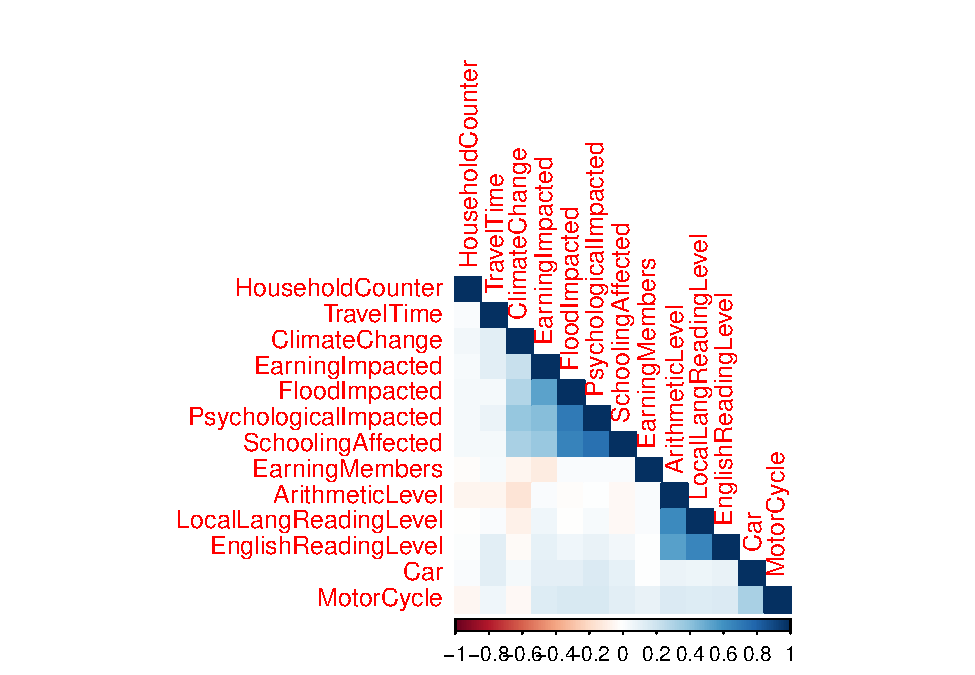
\includegraphics{data_visualization_projectRmd_files/figure-latex/unnamed-chunk-6-1.pdf}

\subsubsection{5.2 Scatter Plot for Children Enrolled vs.~Children
Present by School Type in Each Rural
Region}\label{scatter-plot-for-children-enrolled-vs.-children-present-by-school-type-in-each-rural-region}

\begin{Shaded}
\begin{Highlighting}[]
\CommentTok{\# {-}{-}{-} Children Enrolled vs. Children Present by SchoolType in Each Rural Region {-}{-}{-}}

\NormalTok{children\_by\_school }\OtherTok{\textless{}{-}}\NormalTok{ child\_house\_school\_filtered }\SpecialCharTok{\%\textgreater{}\%} \CommentTok{\#Creating a new variable to manipulate the data easily without affecting the original dataset}
  \FunctionTok{select}\NormalTok{(RNAME, SchoolType, ChildrenEnrolled, ChildrenPresent) }\SpecialCharTok{\%\textgreater{}\%}
  \FunctionTok{filter}\NormalTok{(ChildrenEnrolled }\SpecialCharTok{\textless{}} \DecValTok{900}\NormalTok{, ChildrenPresent }\SpecialCharTok{\textless{}} \DecValTok{900}\NormalTok{) }\SpecialCharTok{\%\textgreater{}\%}  \CommentTok{\# Filter out high values}
  \FunctionTok{filter}\NormalTok{(}\SpecialCharTok{!}\FunctionTok{is.na}\NormalTok{(SchoolType))  }\CommentTok{\# Filter out missing values}

\NormalTok{children\_by\_school }\SpecialCharTok{\%\textgreater{}\%}
  \FunctionTok{ggplot}\NormalTok{(}\FunctionTok{aes}\NormalTok{(}\AttributeTok{x =}\NormalTok{ ChildrenEnrolled, }\AttributeTok{y =}\NormalTok{ ChildrenPresent)) }\SpecialCharTok{+}
  \FunctionTok{geom\_point}\NormalTok{(}\FunctionTok{aes}\NormalTok{(}\AttributeTok{color =}\NormalTok{ SchoolType), }\AttributeTok{alpha =} \FloatTok{0.5}\NormalTok{) }\SpecialCharTok{+}
  \FunctionTok{geom\_smooth}\NormalTok{(}\AttributeTok{method =} \StringTok{"lm"}\NormalTok{) }\SpecialCharTok{+} \CommentTok{\# Adds a linear regression line}
  \FunctionTok{facet\_wrap}\NormalTok{(}\SpecialCharTok{\textasciitilde{}}\NormalTok{ RNAME) }\SpecialCharTok{+}
  \FunctionTok{scale\_x\_log10}\NormalTok{() }\SpecialCharTok{+} \CommentTok{\# Using log scale for x{-}axis to allow for wide range of values to be distributed effectively}
  \FunctionTok{scale\_y\_log10}\NormalTok{() }\SpecialCharTok{+} \CommentTok{\# Using log scale for y{-}axis to allow for wide range of values to be distributed effectively}
  \FunctionTok{labs}\NormalTok{(}\AttributeTok{title =} \StringTok{"Children Enrolled vs. Children Present by SchoolType in Each Rural Region"}\NormalTok{,}
       \AttributeTok{x =} \StringTok{"Children Enrolled"}\NormalTok{,}
       \AttributeTok{y =} \StringTok{"Children Present at the time of survey"}\NormalTok{) }\SpecialCharTok{+}
  \FunctionTok{theme\_modern}\NormalTok{()}
\end{Highlighting}
\end{Shaded}

\begin{verbatim}
## `geom_smooth()` using formula = 'y ~ x'
\end{verbatim}

\includegraphics{data_visualization_projectRmd_files/figure-latex/unnamed-chunk-7-1.pdf}
\#\#\# 5.3 Bar Graph for Students Enrolled in Co-Ed vs Single-Gender
Schools

\begin{Shaded}
\begin{Highlighting}[]
\FunctionTok{ggplot}\NormalTok{(child\_house\_school\_filtered, }\FunctionTok{aes}\NormalTok{(}\AttributeTok{x =}\NormalTok{ SingleOrCoEdSchool)) }\SpecialCharTok{+}
  \FunctionTok{geom\_bar}\NormalTok{(}\AttributeTok{fill =} \StringTok{"lightblue"}\NormalTok{) }\SpecialCharTok{+}
  \FunctionTok{labs}\NormalTok{(}\AttributeTok{title =} \StringTok{"Number of Students Enrolled in Co{-}Ed vs Single{-}Gender Schools"}\NormalTok{, }\AttributeTok{x =} \StringTok{"School Type"}\NormalTok{, }\AttributeTok{y =} \StringTok{"Count"}\NormalTok{) }\SpecialCharTok{+}
  \FunctionTok{theme\_modern}\NormalTok{()}
\end{Highlighting}
\end{Shaded}

\includegraphics{data_visualization_projectRmd_files/figure-latex/unnamed-chunk-8-1.pdf}

\subsubsection{5.4 Bar Graph Showing the Proportion of Psychological
Impact by Level of Flood
Impact}\label{bar-graph-showing-the-proportion-of-psychological-impact-by-level-of-flood-impact}

\begin{Shaded}
\begin{Highlighting}[]
\FunctionTok{ggplot}\NormalTok{(child\_house\_school\_filtered, }\FunctionTok{aes}\NormalTok{(}\AttributeTok{x =}\NormalTok{ FloodImpacted, }\AttributeTok{fill =}\NormalTok{ PsychologicalImpacted)) }\SpecialCharTok{+}
  \FunctionTok{geom\_bar}\NormalTok{(}\AttributeTok{position =} \StringTok{"fill"}\NormalTok{) }\SpecialCharTok{+}  \CommentTok{\# Creates a stacked bar chart}
  \FunctionTok{coord\_flip}\NormalTok{() }\SpecialCharTok{+}  \CommentTok{\# Flips the x and y axes}
  \FunctionTok{labs}\NormalTok{(}\AttributeTok{title =} \StringTok{"Proportion of Psychological Impact by Flood Impact"}\NormalTok{, }\AttributeTok{x =} \StringTok{"Flood Impact"}\NormalTok{, }\AttributeTok{y =} \StringTok{"Proportion"}\NormalTok{) }\SpecialCharTok{+}
  \FunctionTok{theme\_modern}\NormalTok{()}
\end{Highlighting}
\end{Shaded}

\includegraphics{data_visualization_projectRmd_files/figure-latex/unnamed-chunk-9-1.pdf}

\subsubsection{5.5 Bar Graph Showing the Proportion of Earning Impacted
by Levels of Climate Change
Awareness}\label{bar-graph-showing-the-proportion-of-earning-impacted-by-levels-of-climate-change-awareness}

\begin{Shaded}
\begin{Highlighting}[]
\FunctionTok{ggplot}\NormalTok{(child\_house\_school\_filtered, }\FunctionTok{aes}\NormalTok{(}\AttributeTok{x =}\NormalTok{ ClimateChange, }\AttributeTok{fill =}\NormalTok{ EarningImpacted)) }\SpecialCharTok{+}
  \FunctionTok{geom\_bar}\NormalTok{(}\AttributeTok{color =} \StringTok{"black"}\NormalTok{, }\AttributeTok{position =} \StringTok{"fill"}\NormalTok{) }\SpecialCharTok{+}  \CommentTok{\# Creates a stacked bar chart}
  \FunctionTok{coord\_flip}\NormalTok{() }\SpecialCharTok{+}  \CommentTok{\# Flips the x and y axes}
  \FunctionTok{labs}\NormalTok{(}\AttributeTok{title =} \StringTok{"Proportion of Earning Impact by Climate Change Awareness"}\NormalTok{, }\AttributeTok{x =} \StringTok{"Climate Change Awareness"}\NormalTok{, }\AttributeTok{y =} \StringTok{"Proportion"}\NormalTok{) }\SpecialCharTok{+}
  \FunctionTok{theme\_modern}\NormalTok{()}
\end{Highlighting}
\end{Shaded}

\includegraphics{data_visualization_projectRmd_files/figure-latex/unnamed-chunk-10-1.pdf}

\subsubsection{5.6 Distribution of Arithmetic Levels by Medium of
Instruction for the Primary
Grades}\label{distribution-of-arithmetic-levels-by-medium-of-instruction-for-the-primary-grades}

\begin{Shaded}
\begin{Highlighting}[]
\CommentTok{\# Distribution of Arithmetic Levels by Medium of Instruction for the Primary Grades}
\NormalTok{grade\_arithmetic\_medium }\OtherTok{\textless{}{-}}\NormalTok{ child\_house\_school\_filtered }\SpecialCharTok{\%\textgreater{}\%}
  \FunctionTok{select}\NormalTok{(InstructionMedium, ArithmeticLevel, Grades) }\SpecialCharTok{\%\textgreater{}\%}
  \FunctionTok{filter}\NormalTok{(Grades }\SpecialCharTok{\%in\%} \FunctionTok{c}\NormalTok{(}\StringTok{"Grade 1"}\NormalTok{, }\StringTok{"Grade 2"}\NormalTok{, }\StringTok{"Grade 3"}\NormalTok{, }\StringTok{"Grade 4"}\NormalTok{, }\StringTok{"Grade 5"}\NormalTok{)) }\SpecialCharTok{\%\textgreater{}\%}  \CommentTok{\# Filter out only the first five grades to focus on primary levels}
  \FunctionTok{filter}\NormalTok{(InstructionMedium }\SpecialCharTok{!=} \StringTok{"Others"}\NormalTok{)  }\CommentTok{\# Filter out the "Others" category}
\FunctionTok{ggplot}\NormalTok{(grade\_arithmetic\_medium, }\FunctionTok{aes}\NormalTok{(}\AttributeTok{x =}\NormalTok{ InstructionMedium, }\AttributeTok{fill =}\NormalTok{ ArithmeticLevel)) }\SpecialCharTok{+}
  \FunctionTok{geom\_bar}\NormalTok{(}\AttributeTok{color =} \StringTok{"black"}\NormalTok{, }\AttributeTok{position =} \StringTok{"fill"}\NormalTok{) }\SpecialCharTok{+}  \CommentTok{\# Stacks the bars proportionally}
  \FunctionTok{facet\_wrap}\NormalTok{(}\SpecialCharTok{\textasciitilde{}}\NormalTok{ Grades) }\SpecialCharTok{+}  \CommentTok{\# Facets the plot by Grades}
  \FunctionTok{labs}\NormalTok{(}\AttributeTok{title =} \StringTok{"Distribution of Arithmetic Levels by Medium of Instruction for Primary Grades"}\NormalTok{, }
       \AttributeTok{x =} \StringTok{"Medium of Instruction (English, Sindhi, Urdu)"}\NormalTok{, }
       \AttributeTok{y =} \StringTok{"Proportion of Students Reaching the Arithmetic Level"}\NormalTok{) }\SpecialCharTok{+}
  \FunctionTok{theme\_modern}\NormalTok{()}
\end{Highlighting}
\end{Shaded}

\includegraphics{data_visualization_projectRmd_files/figure-latex/unnamed-chunk-11-1.pdf}

\section{6. Discussion}\label{discussion}

The bar graph for school type distribution shows that the majority of
children are enrolled in government schools compared to private schools.
Since the observations are concentrated in rural areas instead of urban,
this distribution tends well to the hypothesis that the majority
students in rural areas access education through government (public)
schools.

The scatter plot for children enrolled vs.~children present by school
type in each rural region shows that there is a positive correlation
between the number of children enrolled and the number of children
present in both government and private schools. The linear regression
line indicates that as the number of children enrolled increases, the
number of children present also increases. This suggests that the
schools are able to maintain a good attendance rate for the children
enrolled. This is remarkable as it shows that the schools have been
resilient in dealing with the after effects of the 2022 floods in
Pakistan which resulted in significant impact on the infrastructure of
schools, and schooling outcomes of children.

The stacked bar graphs for understanding the relationship between the
climate change awareness and the proportion of households experiencing
an earning impact, and the flood impact and the proportion of
psychological impact, show that there is a significant proportion of
households experiencing an earning impact due to climate change. This is
a concerning finding as it suggests that the awareness of climate change
is not translating into effective policy measures to mitigate the impact
on the earning capacity of households. Similarly, the proportion of
psychological impact due to flood impact is also significant, which
indicates that the psychological well-being of individuals is being
affected by the natural disasters in the region.

The distribution of arithmetic levels by the medium of instruction for
the primary grades shows that the majority of students are able to reach
the arithmetic level of numbers 1-9 in the first five grades. This is a
positive finding as it suggests that the students are able to grasp the
basic arithmetic concepts in the early grades. However, there is a need
to focus on improving the arithmetic levels for the higher grades to
ensure that the students are able to build on their foundational
knowledge and skills.The performance of schools based on the medium of
instruction is also a significant finding as it shows that the students
are able to perform comparatively similar in arithmetic for all three
major mediums. This goes against the common perception that students
perform better in English medium schools compared to Urdu and Sindhi
medium schools. However, more research is needed to understand the
factors that contribute to the performance of students in different
mediums of instruction.

\end{document}
